\documentclass[a4paper, 12pt, titlepage,oneside,drop]{kthesis}
\usepackage{a4wide}            
\usepackage[T1]{fontenc}
\usepackage{lmodern}
\usepackage[utf8]{inputenc}    
\usepackage[swedish,english]{babel}
\usepackage{cite}
\usepackage[pdftex]{graphicx}
\usepackage{epstopdf}
\usepackage{graphicx}   % For eps figures
\usepackage{csvsimple}
\usepackage{amsmath}
\usepackage{multirow}
\usepackage{rotating}
\usepackage{amsmath}
\usepackage{amsfonts}
\usepackage{amssymb}
\usepackage{amsbsy}
\pagestyle{headings}
\usepackage{color}
\usepackage{graphicx}
\usepackage{epsfig}
\usepackage{float}
\newtheorem{thm}{Theorem}
\usepackage{tikz}
\usetikzlibrary{shapes,arrows}
\usepackage[hang,indention=-0.5cm,width=14cm,font=small,labelfont=bf,labelsep=period]{caption}
\usepackage{palatino}
\usepackage{fixltx2e}
\usepackage{siunitx}
\setlength{\parskip}{6pt}  % 12 pt = hopp mellan stycken
\setlength{\parindent}{0pt} % 0 pt  = indrag
\makeatletter
\newcommand{\rmnum}[1]{\romannumeral #1}
\newcommand{\Rmnum}[1]{\expandafter\@slowromancap\romannumeral #1@}
\makeatother

%And here the document begins!

\begin{document}
\def\hath{\hat{H}}
\def\wf {\Psi(\{ {\textbf r}_{\textit i}, {\textbf R}_{\textit I} \})}
\def\wfbo{\Psi_{{\textit BO}}({{\textbf r}_{{\textit i}}},{\textbf R} )}
\def\wfh{\Psi_{{\textit H}}(\{ {\textbf r}_{{\textit i}}\})}
\def\wfks{\Psi_{{\textit KS}}(\{ {\textbf r}_{{\textit i}}\})}
\def\wfhit<#1>{\Psi_{{\textit H}}^{#1}({{\textbf r}_{{\textit i}}})}
\def\bwf<#1><#2>{\phi_{#1}({\textbf r}_{#2})}
\def\bwfn<#1><#2>{\phi_{#1}({\textbf r}{#2})}
\def\wfbloch<#1><#2>{\Psi_{#1,#2}({\textbf r})}
\def\ubloch<#1><#2>{u_{#1,#2}({\textbf r})}
\def\ebloch<#1><#2>{E_{#1,#2}}
\def\bwfc<#1><#2><#3>{\phi_{#1}^{#3}({\textbf r}_{#2})}
\def\sumi<#1> {\sum\limits_{\textit #1}}
\def\sumij<#1><#2> {\sum\limits_{\textit #1,#2}}
\def\suminj<#1><#2> {\sum\limits_{{\textit #1} \neq {\textit #2}}}
\def\coefkhe{-\frac{\hbar^2}{2 m_{\textit e}}}
\def\coefkhn{-\frac{\hbar^2}{2 M_\textit{I}}}
\def\nablaia<#1> {{\nabla}_{\textit{#1}}^{2}}
\def\moperater{-i\hbar \nabla}
\def\sumg<#1>{{\sum\limits_{{#1}}}}    
\def\sumlm<#1><#2>{\sum\limits_{{#1}{#2}}}
\def\coeff<#1><#2><#3>{C_{#1,{\textbf k_0} +\textbf{#2}}^{#3}}      %C_{j,k_0+G}^{*}
\def\expkg<#1><#2>{e^{i(\textbf{#1}+\textbf{#2})\textbf{r}}}          %exp{i(k+G)r}
\def\expg<#1>{e^{i{\textbf #1} {\textbf r}}}                         %exp{iGr}
%\def\bwf<#1>{\phi_{\textbf{k_0}+\textbf{#1}}^{\textbf{APW}}(\textbf{r})}          %phi_{k_0+G}  
\def\chig<#1>{{\chi_{\textbf kk_0}(\textbf{#1})}}                  %chi_{kk_0}{G}
%\def\hath{ | \hat{H} | }           
\def\kplusg<#1><#2>{(\textbf{#1}+\textbf{#2})}                    % k+G 
\def\radiaf<#1><#2>{f_{{\ell}^{\prime}{m}^{\prime}} (r_{\alpha},\textbf{#1+#2})}    % f(r,k+G)
\def\radiafc<#1><#2><#3>{f_{{\ell}^{\prime}{m}^{\prime}}^{#3} (r_{\alpha},\textbf{#1+#2})}    % f(r,k+G)
\def\bradiaf{u^{\alpha}_{q,\ell^{\prime}}(r_{\alpha},E_{\ell^{\prime}})}              %u(r_\alpha) did not contain the Energy
\def\sphfr<#1><#2><#3> {{Y_{#1}^{#3}(\hat{\textbf{#2}}_{\alpha})}}                             %Y_{lm}(\hat{r})
\def\sphfq<#1><#2><#3> {{Y_{#1}^{#3}(\widehat{{\textbf{#2}}})}}                             %Y_{lm}(\hat{q})
\def\gaucoe{C_{{\ell{m}},{\ell^{\prime}m^{\prime}},{\ell^{\prime\prime}m^{\prime\prime}}}}  %Gaunt coefficient
\def\potvgir{V_{\textbf G^{\prime\prime} }}                                %V{G}
\def\potvmt{V^{\alpha}_{{\ell}^{\prime\prime}{m}^{\prime\prime}} (r_{\alpha})}  %V{lm,r}     
\def\fracatom<#1> {e^{i \textbf{#1} \textbf R^\alpha }}   % exp(iq\def\nablai2<#1> {{\nabla}_{\textit{#1}}^{2}}R)
\def\bessf<#1>{j_{\ell}({#1}r_{\alpha})}     %j_l(kr)
\def\dr{\mathrm{d}\textbf{r}}
\def\chikp<#1><#2>{{\chi_{#1,#2}(\textbf{r})}}  
\newcommand{\se}{Schrödinger equation}
\def\hm{Hamiltonian }
\def\cigs{\mathrm  { CuIn_{1-\textit{x}}Ga_{x}Se_2}}
\def\czts{\mathrm {Cu_2ZnSnS_2} } 
\def\cztse{\mathrm { Cu_2ZnSnSe_2}}
\def\cztsse{\mathrm  { CuZnSn(S_{1-\textit{x}}Se_{x})_4}}


\pagenumbering{roman}
\setcounter{page}{1}

\begin{center}




 
\epsfig{file=kth_svv_indu_eng_manage.eps,width=4 cm}
  \vspace{5 cm}





  \vspace{12pt}
  \textsc{\LARGE{\textbf{{\today}}}}
  \vspace{12pt}

  \vspace{5 cm}

  \textsc{\large{Rongzhen Chen}}


  \vfill 

  \ 

  \large{Doctoral Thesis}
  \\
  \large{School of Industrial Engineering and Management,
  Department of Materials Science and Engineering,
  KTH, Sweden, 2014}

\end{center}

 \thispagestyle{empty}



\newpage
\setcounter{page}{2}
\thispagestyle{empty}
\
\vfill

\begin{flushright}
 Materialvetenskap\\
 KTH\\
ISRN KTH/MSE--12/09--SE+AMFY/AVH
 \hfill SE-100 44 Stockholm\\ ISBN 978-91-7501-313-8  \hfill
Sweden\\
\end{flushright}


\vspace{5mm}

Akademisk avhandling som med tillstånd av Kungliga Tekniska
Högskolan framlägges till offentlig granskning för avläggande av
tenknologie doktorsexamen in materialvetenskap  ???
2014 kl ???? i ??, Materialvetenskap, Kungliga Tekniska
Högskolan,\linebreak Brinellvägen 23, Stockholm.

\vspace{5mm}

\copyright \hspace{3pt} Rongzhen Chen, ???, 2014

\vspace{5mm}

Tryck: Universitetsservice US AB

\newpage


\begin{abstract}

\newpage

\end{abstract}

\newpage
\setcounter{page}{5}

\section*{Preface} \addcontentsline{toc}{chapter}{Preface}

\subsection*{List of included publications:}

\begin{enumerate}
\renewcommand{\labelenumi}{\Roman{enumi}}
%\item{} \textbf{Parameterization of $CuIn_{1−x}Ga_{x}Se_2$ (x = 0, 0.5, and 1) energy bands}
\item{}  \textbf{Parameterization of $\mathbf {CuIn_{1-x}Ga_{x}Se_2}$ (x = 0, 0.5, and 1) energy bands}
\\\textbf{R. Chen} and C. Persson, \textit{Thin Solid Films} {\textbf {519}}, 7503 (2011).



\item{}\textbf{Band-edge density-of-states and carrier concentrations in intrinsic and \textit{p}-type $\mathbf {CuIn_{1-x}Ga_{x}Se_2}$}
\\\textbf{R. Chen} and C. Persson, \textit{J. Appl. Phys.} {\textbf {112}}, 103708 (2012).

\item{} \textbf{Dielectric function spectra at 40 K and critical-point energies for $\mathbf {CuIn_{0.7}Ga_{0.3}Se_2}$}
\\ S.G. Choi, \textbf{R. Chen}, C. Persson, T.J. Kim, S.Y. Hwang, Y. D. Kim, and L. M. Mansfield,
\textit{Appl. Phys. Lett. } {\textbf {101}}, 261903 (2012).

\end{enumerate}
\subsection*{Comment on my own contribution}

\textbf{Paper I:} modeling, analysis of result, literature survey;
the manuscript was written jointly.\\
\textbf{Paper II:} modeling, analysis of result, literature survey; main part of the manuscript was written.\\
\textbf{Paper \Rmnum{3}:} all calculations, analysis of the theoretical part, part of literature survey;
the manuscript was written jointly.\\

\subsection*{Publications not included in the thesis:}
\begin{enumerate}
\renewcommand{\labelenumi}{\Roman{enumi}}
\setcounter{enumi}{3}


\item{}\textbf{Electronic structure and optical properties from first-principles modeling} \\
C. Persson, \textbf{R. Chen}, H. Zhao, M. Kumar, and D. Huang, Chapter in “Copper zinc tin sulphide-based thin film solar cells”,
edited by K. Ito ({\textit John Wiley $\&$ Sons}, ??CITY??, ??2014??); in preparation.


\end{enumerate}

\subsection*{International conference contributions:}
\begin{enumerate}
\renewcommand{\labelenumi}{\Roman{enumi}}
\setcounter{enumi}{4}

\item{} \textbf{Band structure and optical properties of $\mathbf {CuInSe_2}$}
\\ \textbf{R. Chen} and C. Persson, 
\textit{Advanced Materials Research Journal} {\textbf 894}, 254 (2014). \\
\textit{4th Int. Conf. on Adv. Mater. Res (ICAMR-4), Macao, China, 23-24 Jan. 2014.}


\item{} \textbf{Electronic modeling and optical properties of $\mathbf{CuIn_{0.5}Ga_{0.5}Se_2}$ thin film solar cell}
\\ \textbf{R. Chen} and C. Persson,
\textit{J. Appl. Math. \& Phys.} {\textbf 2}, 41 (2014). \\
\textit{Conf. on New Adv. Cond, Matter Phys. (NACMP 2014), Shenzhen, 14-16 Jan 2014.}

\end{enumerate}

\newpage
\setcounter{page}{7}
\setcounter{secnumdepth}{3}
\setcounter{tocdepth}{3}
\tableofcontents

\newpage
\pagenumbering{arabic}
\chapter{Introduction}

With the increasing of energy consumption, more and more energy or power is needed. According to the statistical review of world energy on 2013 (\textbf{Fig. \ref{wpec}}),
the required energy is mainly satisfied by the fossil fuels (mainly coal, petroleum and 
natural gas), with a market share of around 87\%. The total energy consumption is around 12000 million tonnes oil equivalent (METO), which is equivalent with around 15 terawatts. 
Normally lightbulbs in our homes consume around 100 watts of energy, 1 terawatt means is 10 billion of the lightbulbs is lighted at the same time. 
Unfortunately, the fossil fuels is very limited energy and non-renewable resources, one day which is not far from  now it will be dissipated due to the energy consumption growth.

\begin{figure}[H]
\centering
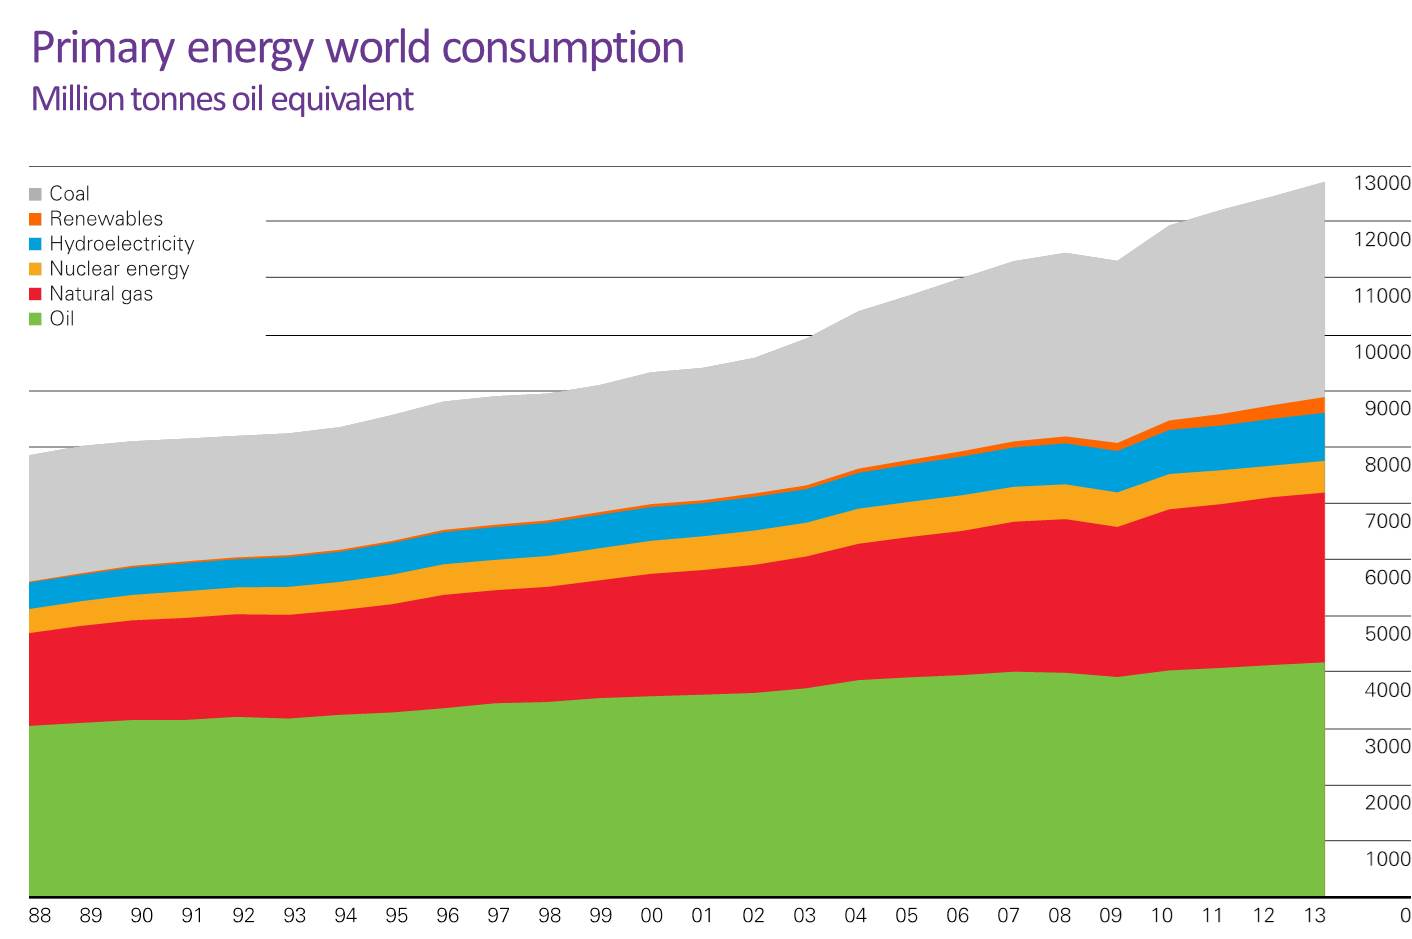
\includegraphics[scale=0.4]{energy.jpg}
\caption{Data is from BP statistical review of world energy 2013, METO means million tonnes oil equivalent.}
\label{wpec}
\end{figure}

By the year of 2050, the total world energy consumption will around double. Therefore, it is urgent to explore more sustainable and healthy energy sources. From \textbf{Fig. \ref{wpec}}, one will notice that renewable energy (mainly solar energy, wind power, hydropower and 
geothermal energy) in 2013 accounts for around 2\% of energy consumption globally. It is important to focus on the renewable energy research from a long term point of view.
The solar energy technologies are one of the hot topic among the renewable energy research considering the point of CO\textsubscript{2} free, reliable energy supply, no cooling water requirement and operation in silence.

The solar energy technologies are the way to produce electricity from the light of the sun. Sunlight is a portion of the radiation by the sun, like infrared, visible,
and ultraviolet light. The spectrum of the sun is more or less a black body with a temperature of about 6000 K (\textbf{Fig. \ref{spectrumsun}}). In photovoltaic field, solar spectrum is represented by Air Mass (AM), 
and the AM1.5 and AM0 are important. AM1.5 is the air mass at a solar zenith angle of 48.19 degree, and AM0 mean the solar spectrum outside of the atmosphere. Generally, the AM1.5 is seen as the reference spectrum in PV field.

\begin{figure}[H]
\centering
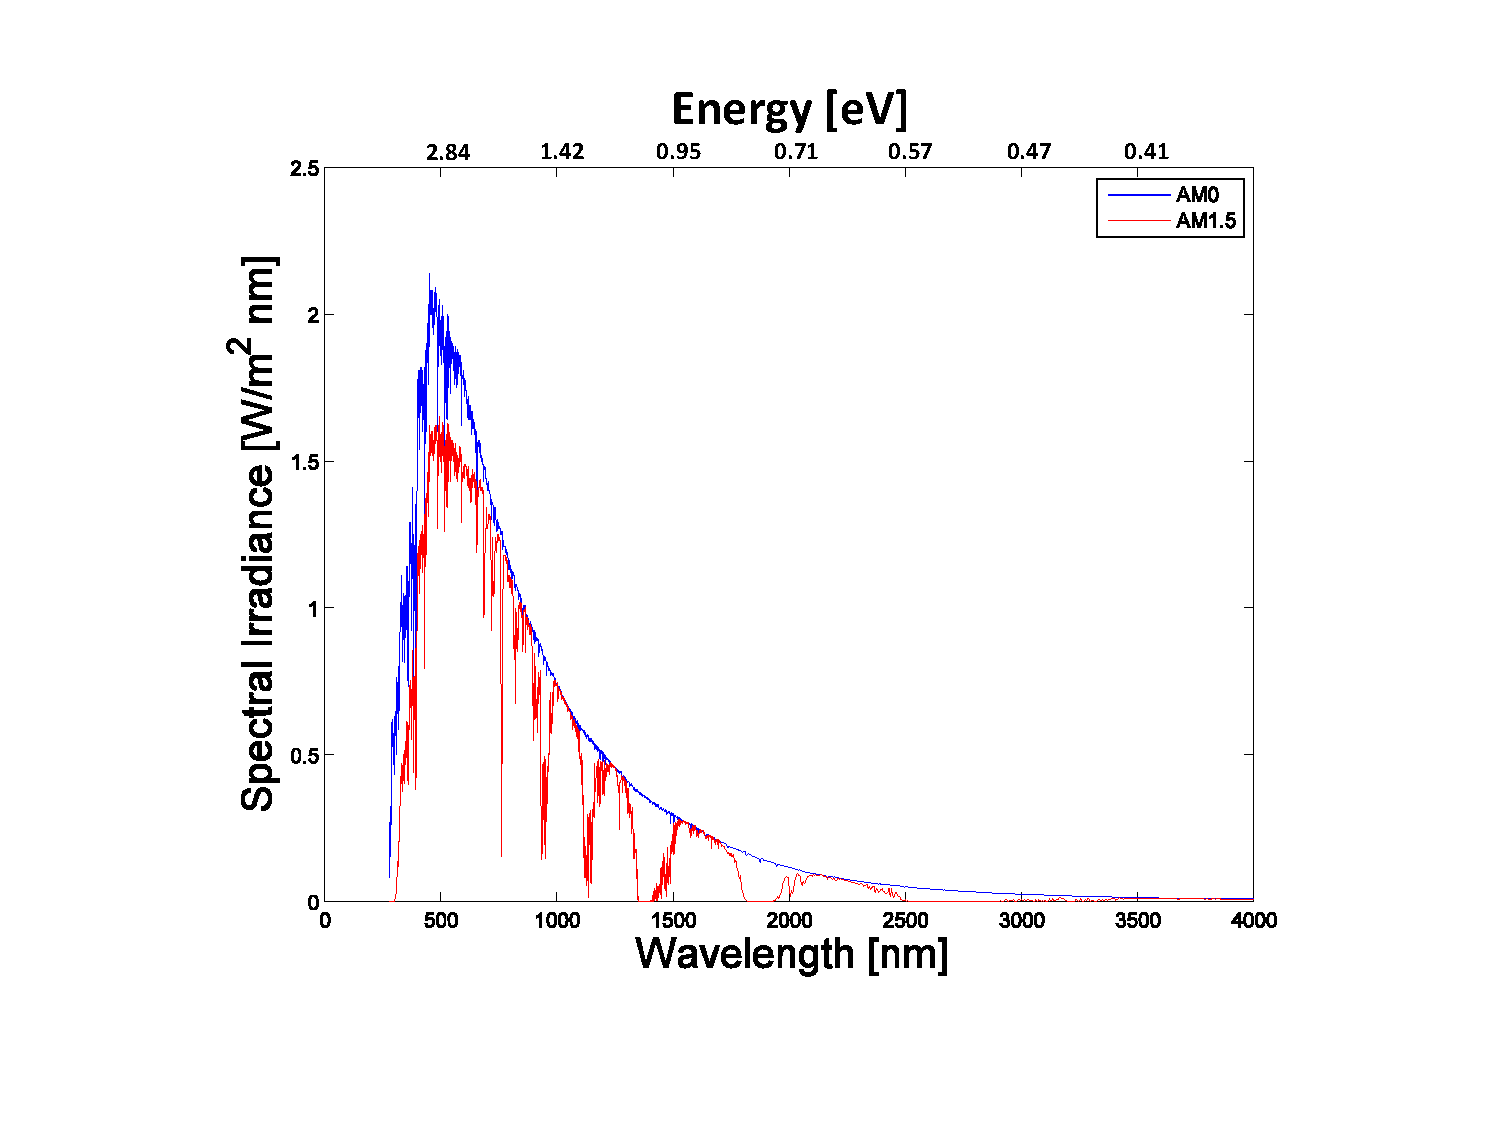
\includegraphics[scale=0.4]{spectrum.pdf}
\caption{Solar irradiance spectrum (Y-axis ??).}
\label{spectrumsun}
\end{figure}

There are mainly three kinds of solar energy technologies. The first one is solar thermal,
which utilizes the flat sunlight collector plates to harness the energy from sunlight to heat water for use in businesses, homes, and pools.
Therefore, the solar thermal collectors do not convert sunlight to electricity directly, but transfer the energy to the water instead. The advangtage is the conversion efficiency 
is relatively higher, however, the price is higher as well and it needs huge amount of cherished water resources. The second one is solar chemical, which takes advantage of solar 
energy by absorbing sunlight in a chemical reaction, and the conversion efficiency is quite low. The last one is solar photovoltaics (solar cell), which is the way
to use solar panels to convert sunlight into electricity. The price is relatively lower compared with solar thermal, and the conversion efficiency is higher than solar chemical. More importantly, it is
environmentally friendly.


\section{Solar cells}
In the worldwide, many reseachers are working on the field of solar cell. Therefore, the conversion efficiency in all different types of solar cell is improved remarkably. 
From \textbf{Fig. \ref{nrel}}, one can notice that the highest efficiency for multijunction cells, crystalline silion cells, thin-film technologies and new emerging cells are around 
44.4\%, 27.6\%, 22.8\% and 16.2\%, respectively. Therefore, the solar cell is a very important and promising way to produce the renewable energy.

\begin{figure}[H]
\centering
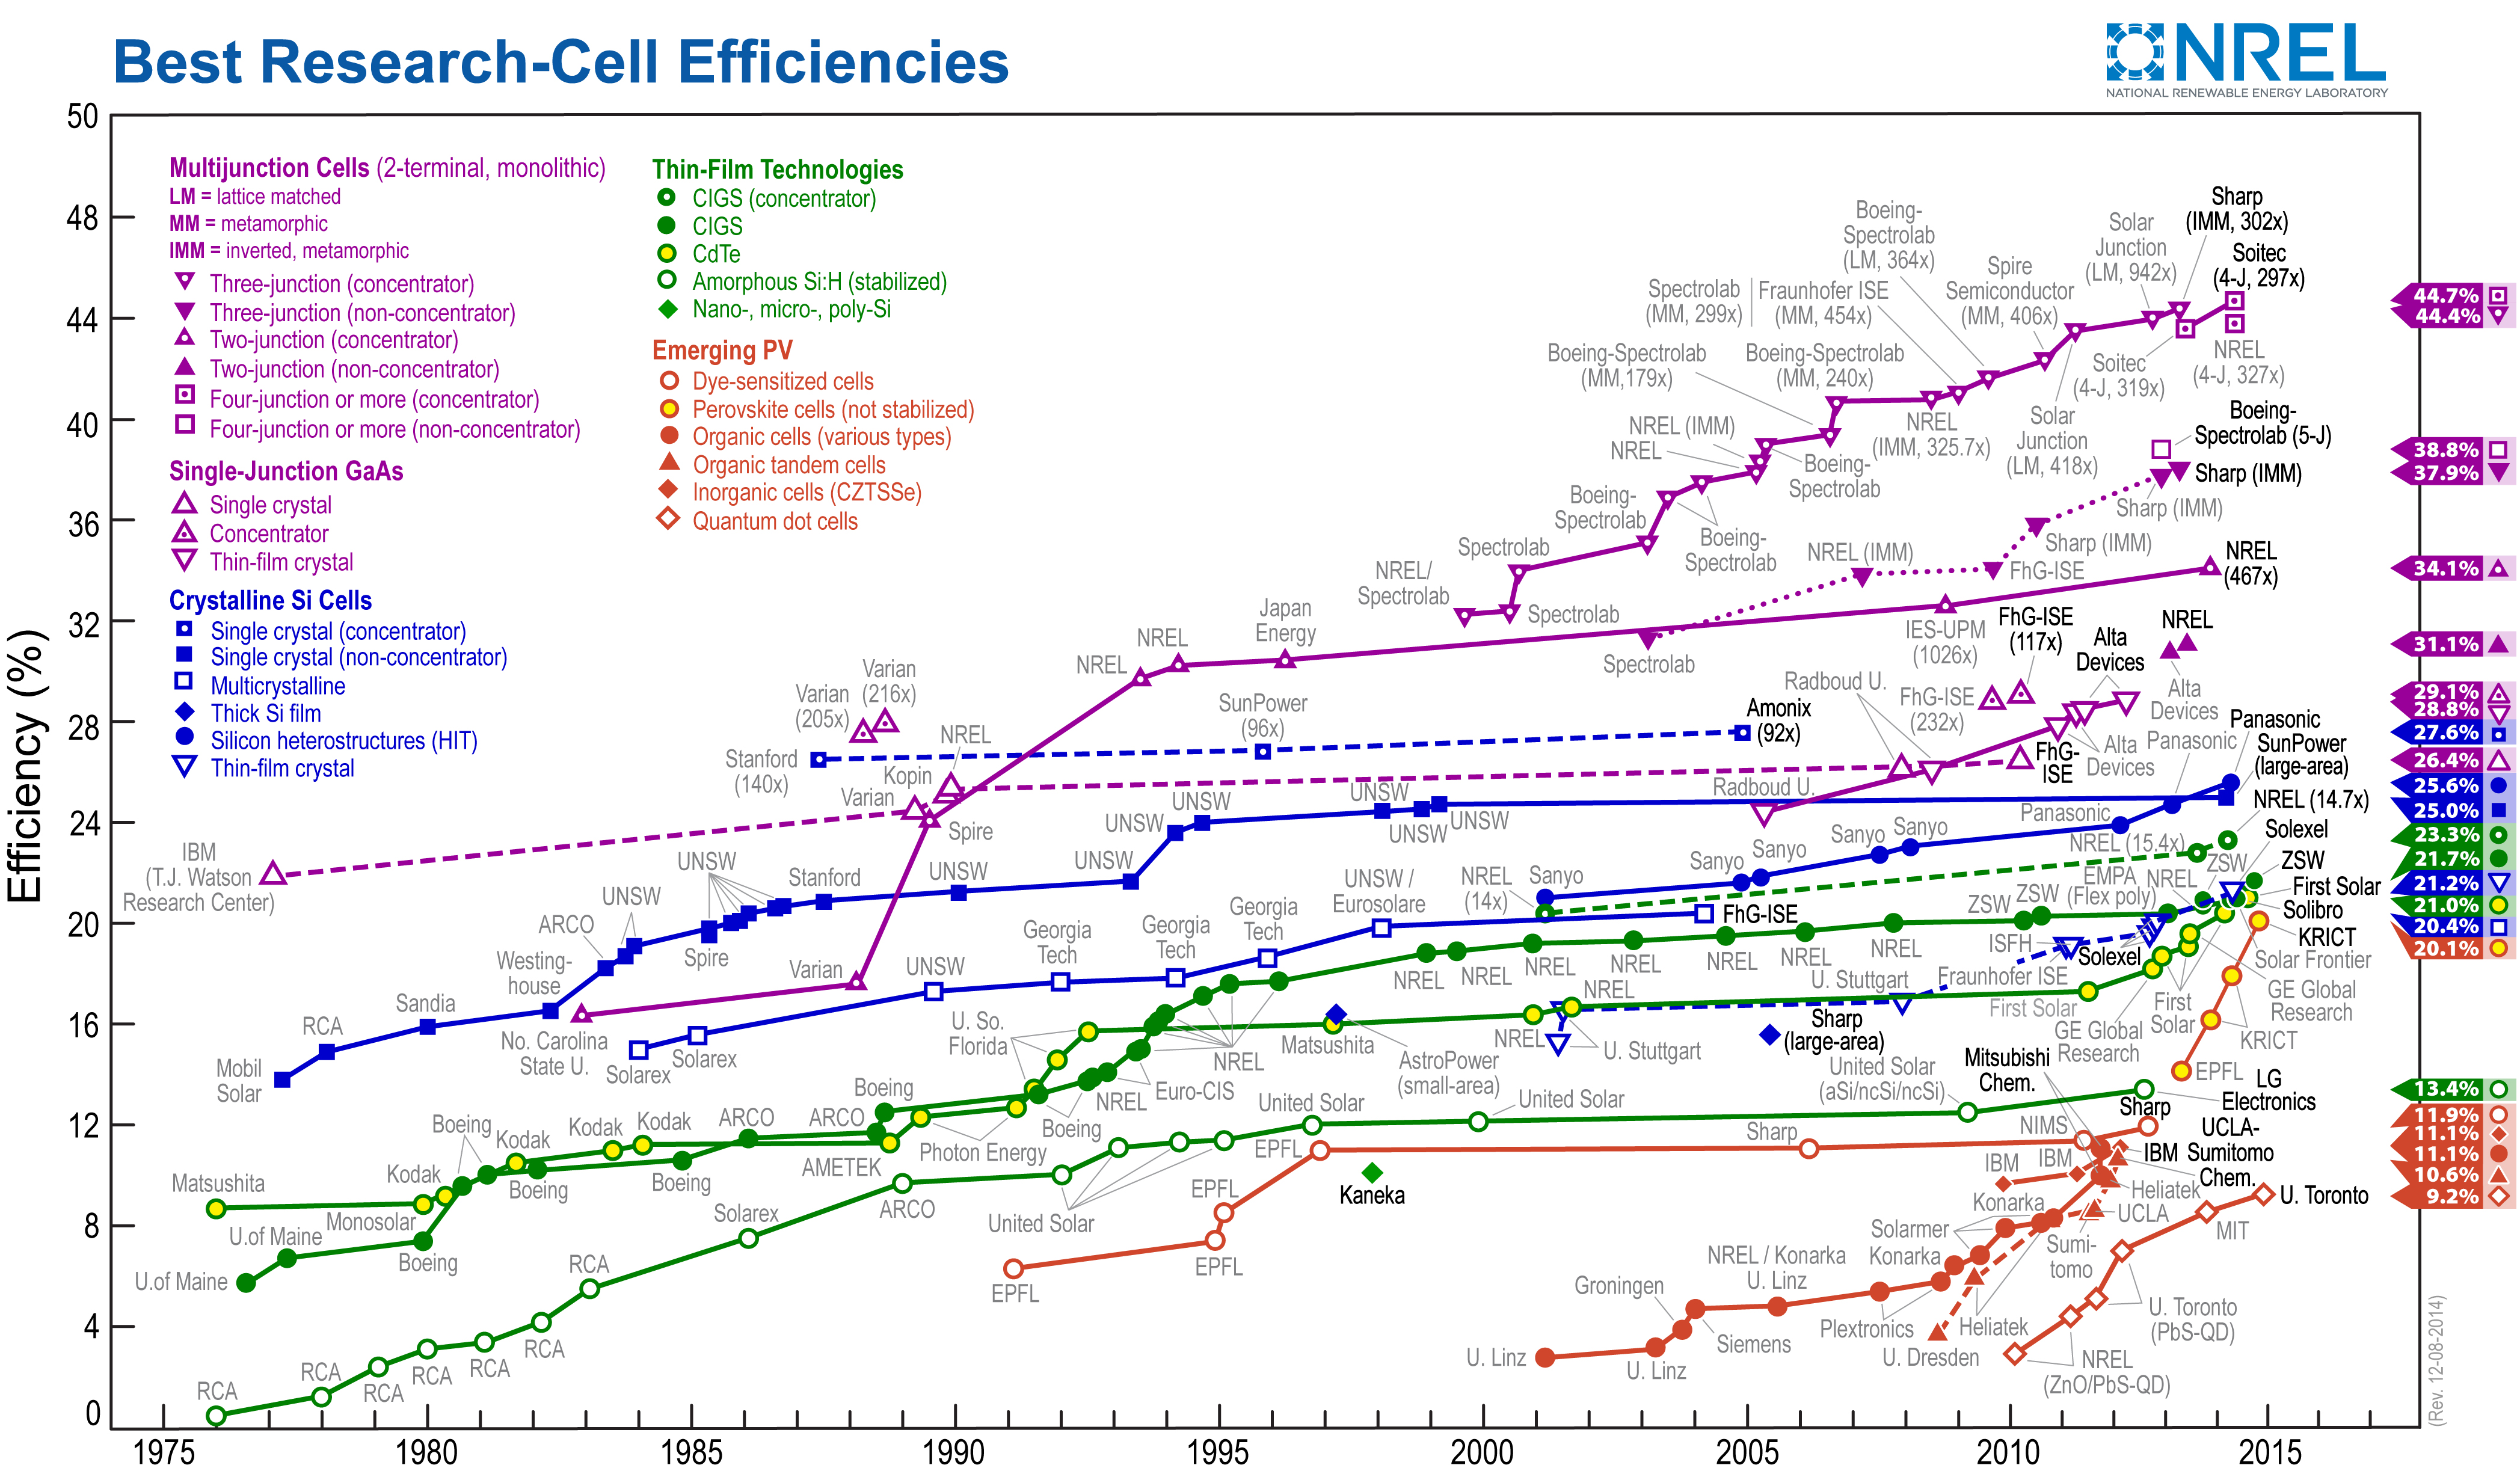
\includegraphics[scale=0.3]{efficiency_chart.jpg}
\caption{Best research-cell efficiencies. Figure is from National Renewable Energy Laboratory (NREL), Golden, Colorado.}
\label{nrel}
\end{figure}

For the multijunction cells, the conversion efficiency is relatively higher compared with others, however, the price is much more expensive as well due to more amount of materials used for production.
Compared with multijunction cells, the crystalline silicon has lower conversion efficiency, but lower price as well. The price for thin film is cheaper than crystalline silicon, however,
the efficiency is little lower than crystalline silicon. The new emerging cells are cheapest compared with all the others type of cells, however, the conversion efficiency is 
relatively lower.


\subsection{Single-junction solar cells}
The p-n junction is the fundamental building block of solar cells. The principle behind the p-n junction needs to be demonstrated in order to better understand the principle of solar cells. 
The single p-n homojunction will be explored in this section.

We will start from the seperate n-type material and p-type material. In the \textbf{Fig. \ref{dopedmaterials}}, the left one is the n-type and p-type material. The n-type of material has many free negatively charged electrons which can move around the material, and there are numbers of positively 
charged immobile donor ions as well. Similarily, the p-type material has many free positively charged holes which can move through the material, and there are numbers of negatively charged immobile acceptor ions as well. However,
the material is still neutral in both n-type and p-type. On the right, the fermi level is shown. The fermi level is close to conduction band for n-type material due to many free negatively charged electrons. Conversely, the fermi level
of p-type material is close to valence band due to the free positively charged holes.

%\begin{figure}[H]
%\centering
%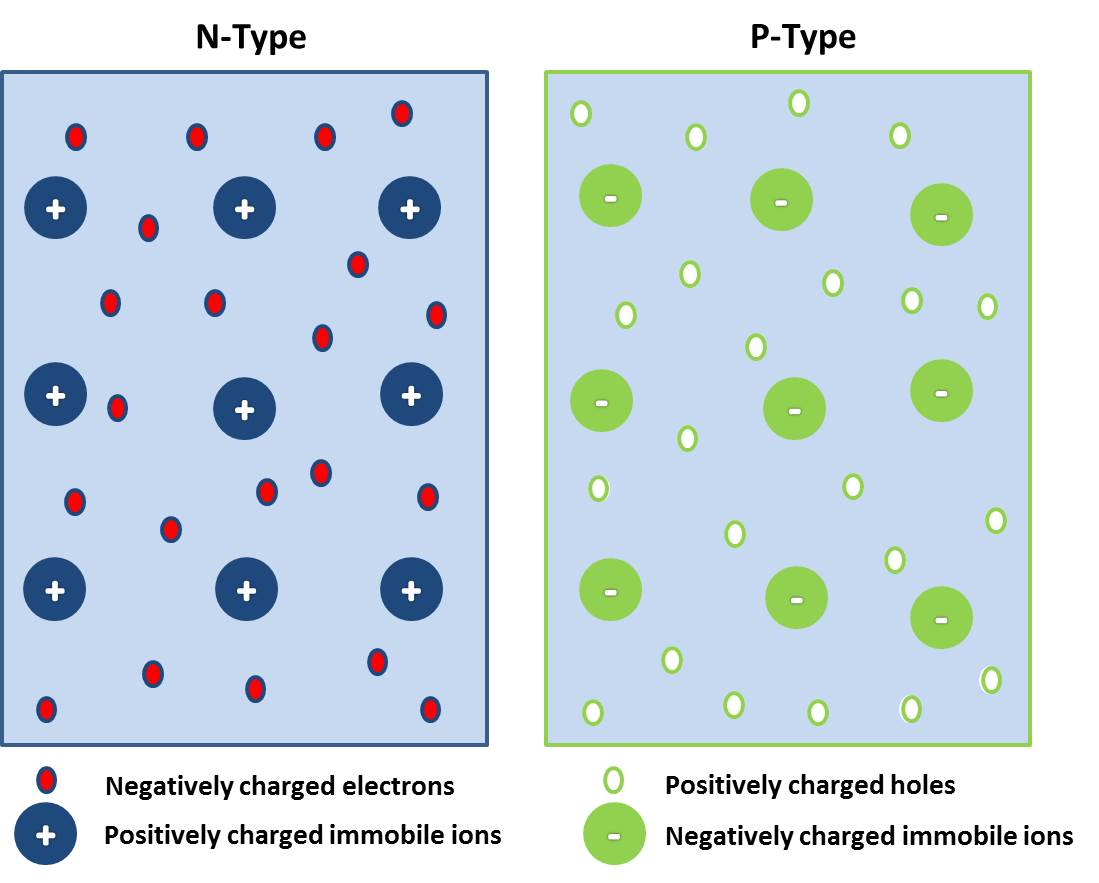
\includegraphics[scale=0.4]{sepratepn.jpg}
%\caption{Doped material (n-type and p-type)}
%\label{dopedmaterials}
%\end{figure}


\begin{figure}[H]
    \begin{center}
            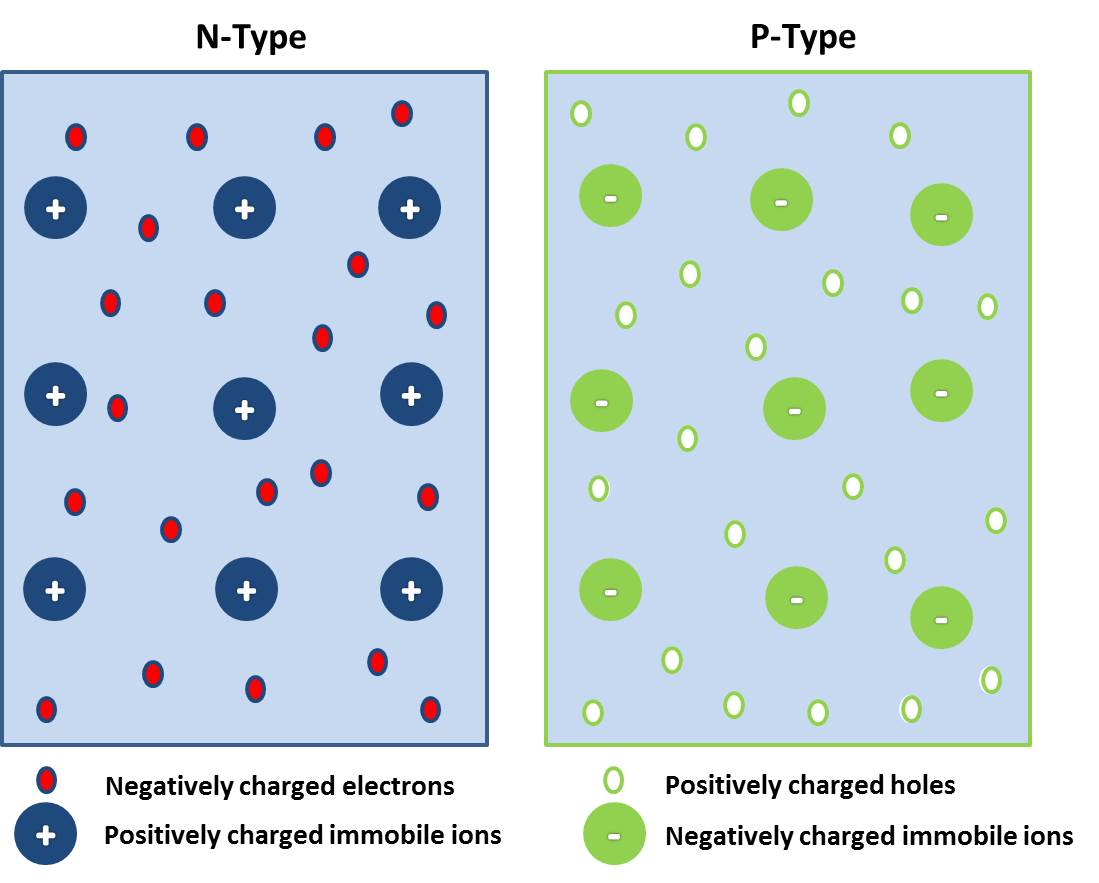
\includegraphics[width=0.4\textwidth,clip]{sepratepn.jpg}
            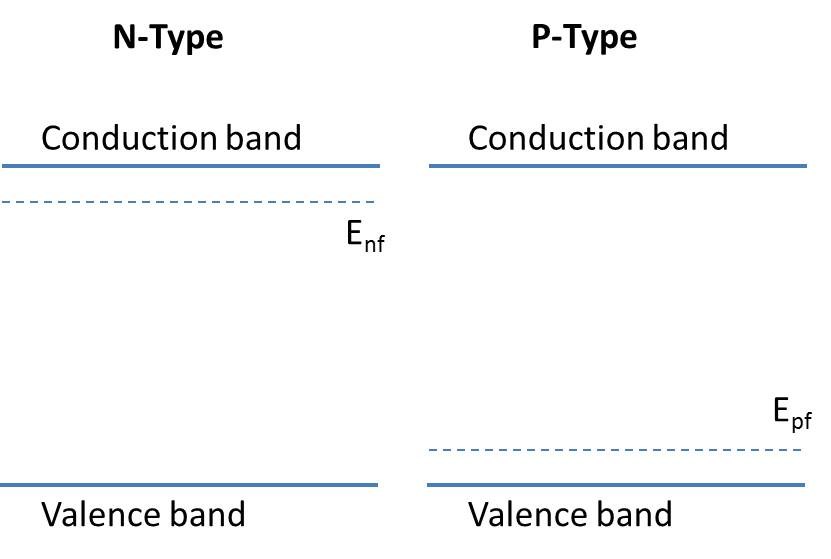
\includegraphics[width=0.4\textwidth,clip]{sepratepn1.jpg}
     \end{center}
    \caption{Left: Doped material (n-type and p-type). Right: Fermi level of n-type and p-type materials}      
    \label{dopedmaterials}
\end{figure}



If the n-type and p-type materials are joined, the free electrons (holes) in the n-type (p-type) material will diffuse into p-type (n-type) material due to the concentration difference (\textbf{Fig. \ref{pnjunction}}). In the region which is near the interface between n-type and
p-type materials, the fixed donor and acceptor ions establish a "build in" electric field which points from n-type material to p-type material. The "build in" electric field will force the electrons (holes) back into the n-type (p-type), at certain
point, the whole material will reach a stable equilibrium. Formation of the "build in" electric field is rather important for the solar cells, even though there is no currect in the material so far. In the following text, the region which establishes
the "build in" electric field is also called space charge region (SCR). The different fermi level for n-type and p-type materials will be equal at the stable equilibrium. 

%\begin{figure}[H]
%\centering
%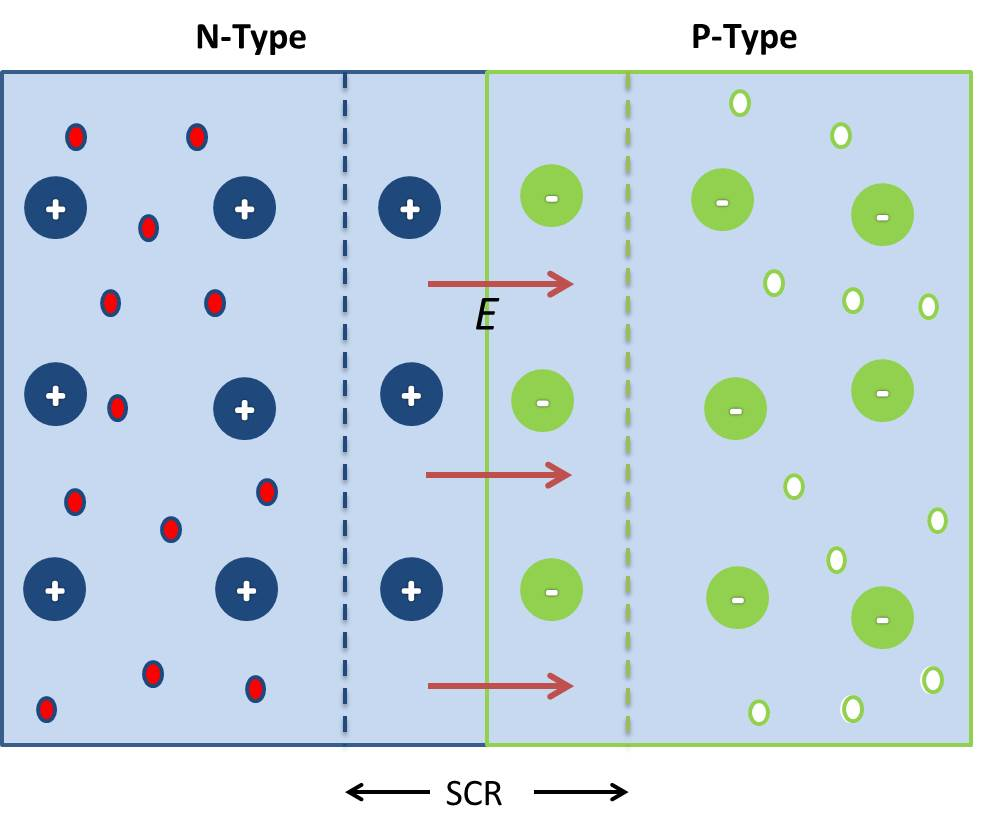
\includegraphics[scale=0.4]{pnjunction.jpg}
%\caption{p-n junction}
%\label{pnjunction}
%\end{figure}


\begin{figure}[H]
    \begin{center}
            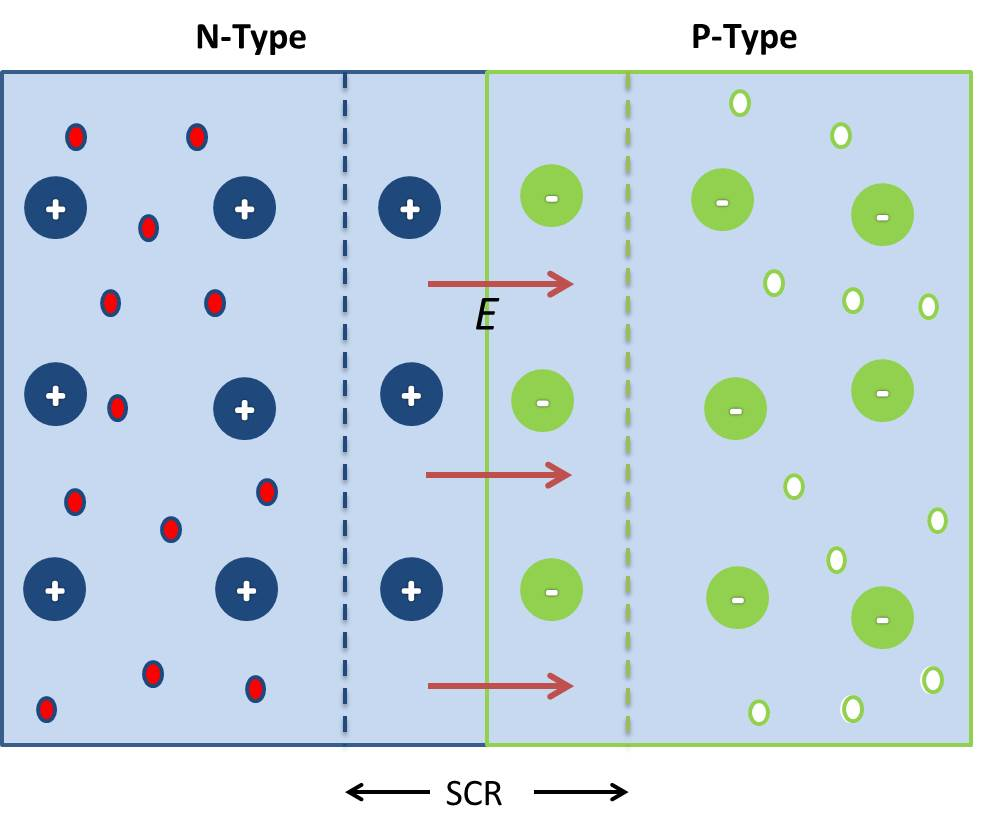
\includegraphics[width=0.4\textwidth,clip]{pnjunction.jpg}
            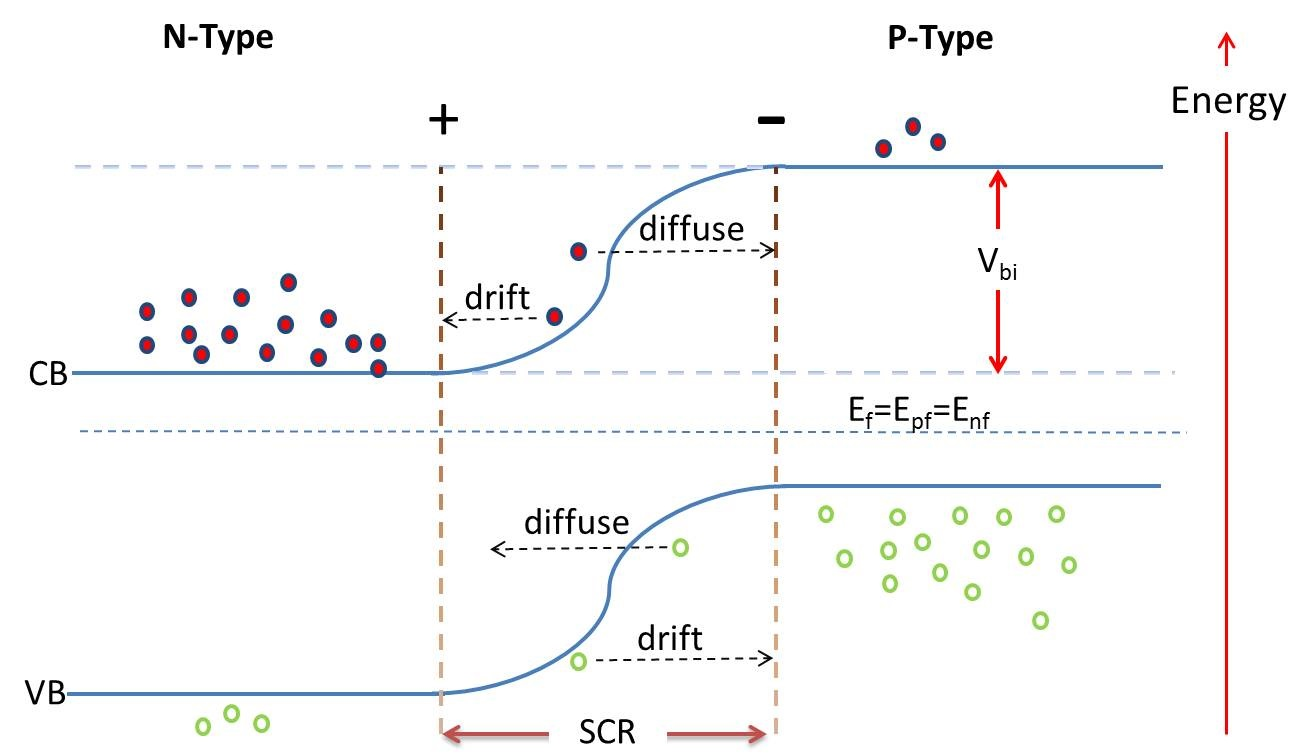
\includegraphics[width=0.4\textwidth,clip]{pnjunction1.jpg}
     \end{center}
    \caption{Left: The p-n homojunction. Right: Fermi level of the p-n homejunction at the equilibrium. }      
    \label{pnjunction}
\end{figure}



\begin{comment}
Before discussing further the p-n junction in the solar cells, the forward and reverse bias will be introduced in the \textbf{Fig. \ref{frb}}. The forward bias means that a negative voltage is applied on the n-type side, and a positive voltage is applied 
on the p-type side. In this case, the SCR will be shrinked. With the increasing of the voltage, the SCR will rather small and the current will flow freely. Conversely, the reverse bias means that a negative voltage is applied on the p-type
side, and a positive voltage is applied on the n-type side. The SCR will become thicker, if the voltage is large enough,  then the whole junction will breakdown and current will flow.

\begin{figure}[H]
    \begin{center}
            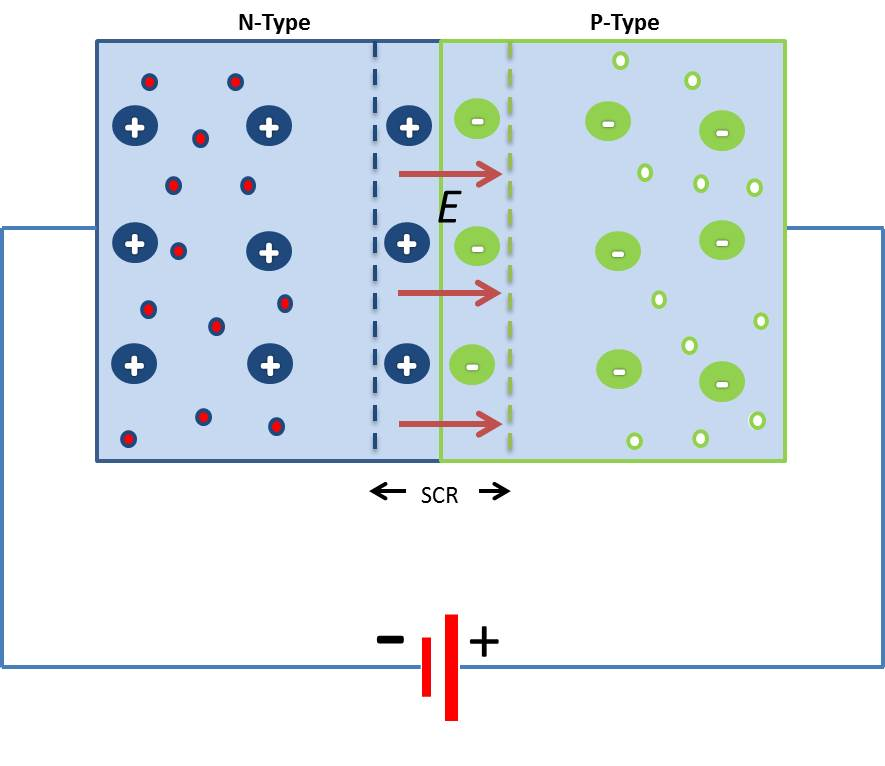
\includegraphics[width=0.4\textwidth,clip]{forwardbias.jpg}
            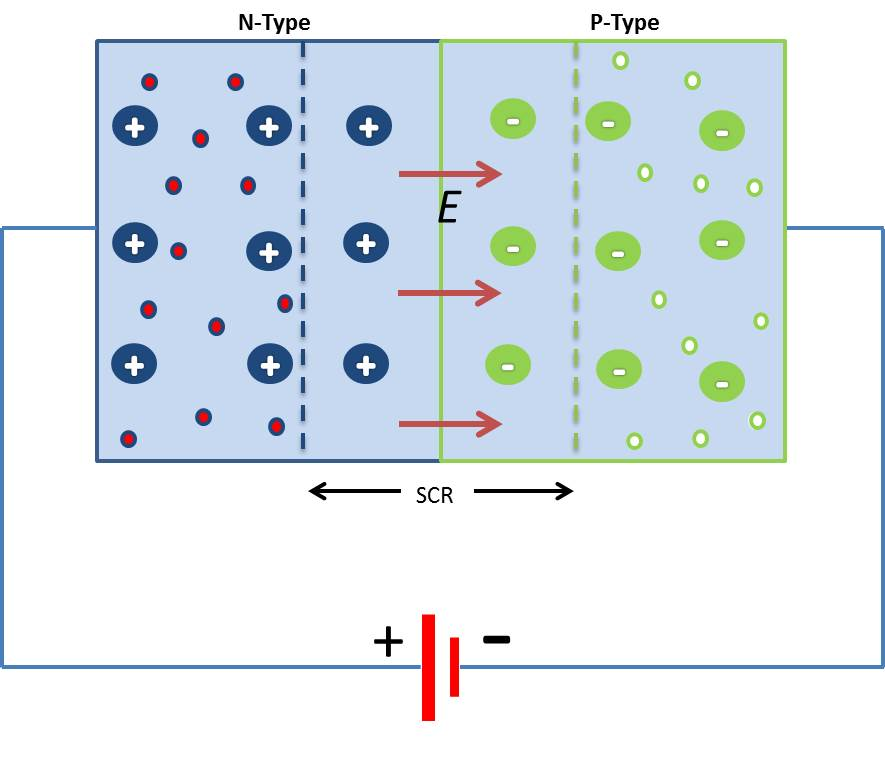
\includegraphics[width=0.4\textwidth,clip]{reversebias.jpg}
     \end{center}
    \caption{Forward and reverse bias}      
    \label{frb}
\end{figure}

\end{comment}


The p-n junction material with and without the illumination is discussed in the \textbf{Fig. \ref{illu}}. If there was a wire with certain resistance connecting the n-type and p-type, there is no current in the wire under the condition of no illumination. However, if the light shines on the whole material, the current will be generated from the 
p-type to the n-type side (conventional current). Because the bond inside the material will be broken under the illumination, which will generate one pair of electron hole. Apparently, there are three regions in the whole junction material where the bonds are possible to be broken, the n-type region, the p-n junction, and
the p-type region. In the either n-type or p-type region, the electron–hole pair will not remain long time,  it is most probable that they will back into the bonded positions again since the pair electron-hole is rather close each other. However, the pair
electron-hole pair will be seperated in the p-n junction region due to the "build in" electric field, therefore, the current will be generated. Actually, the electron-hole pair in the either n-type and p-type also have the chance to diffuse into 
the SCR, it will also contribute the generation of current in this case.

\begin{figure}[H]
\centering
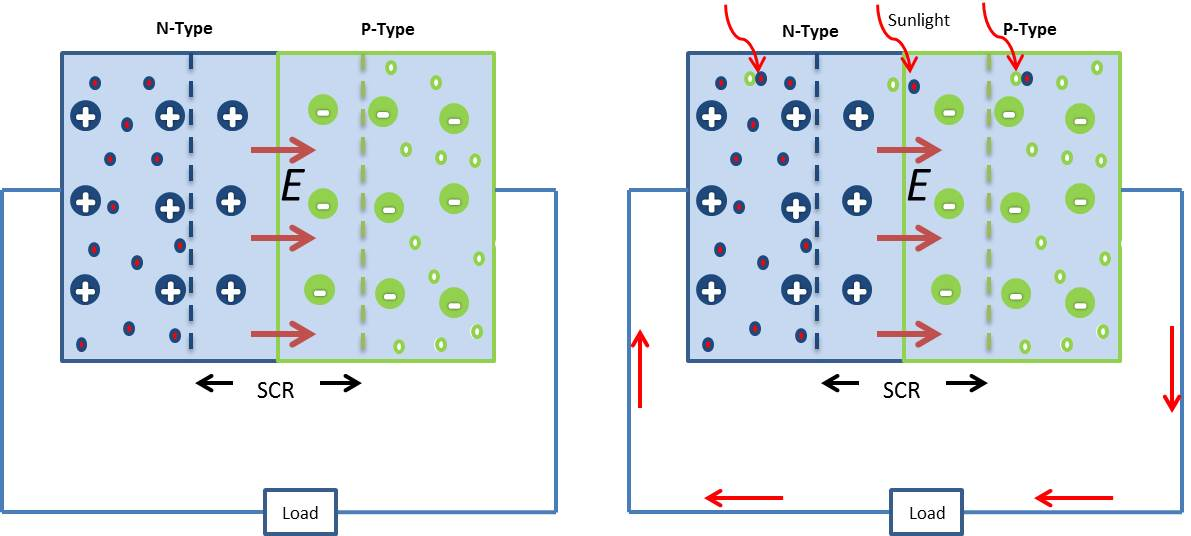
\includegraphics[scale=0.5]{illumination.jpg}
\caption{The p-n junction under illumination}
\label{illu}
\end{figure}

The band-profile of ...


\begin{figure}[H]
\centering
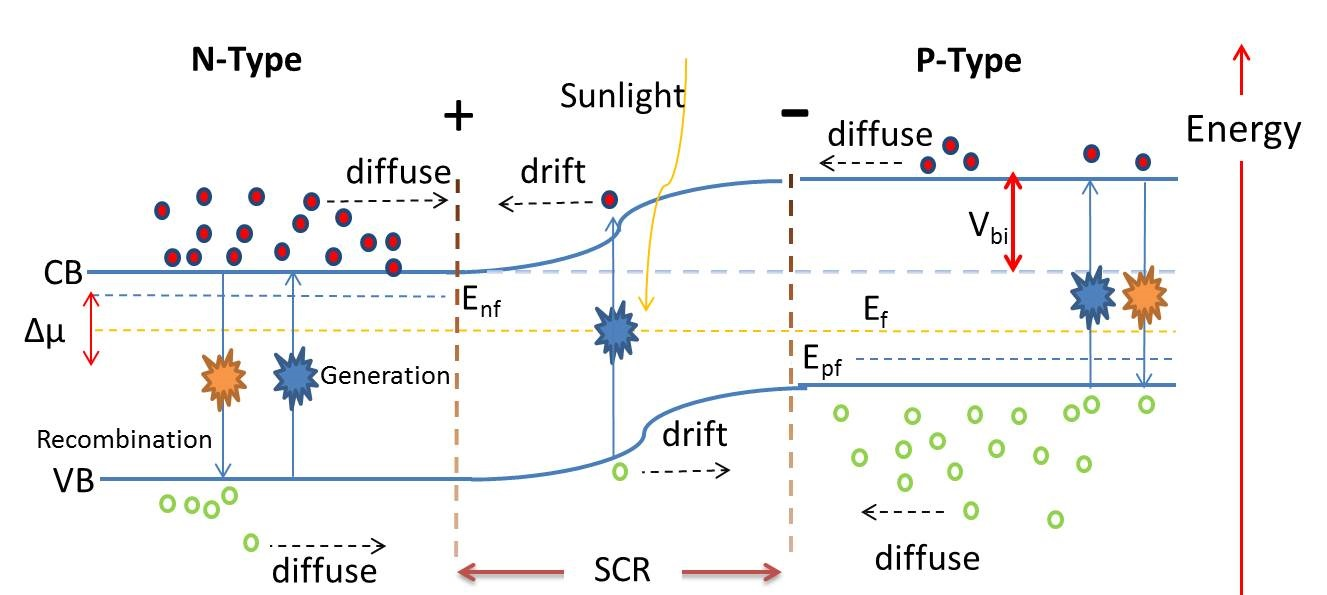
\includegraphics[scale=0.45]{illumination1.jpg}
\caption{Band profile and fermi level of the p-n junction under illumination}
\label{illu1}
\end{figure}


The I-V characteristics is defined in the \textbf{Fig. \ref{ivcharac}} with some important parameters in the solar cells.
The $V_{oc}$ and $I_{sc}$ are the open circuit voltage and short circuit current, respectively. They are the maximum voltage and current when the solar cells are with the illumination conditions.
And $V_{mp}$ and $I_{mp}$ are the voltage and current which will yield the maximum power. The maximum power generated by the solar cells is $P_{out}=V_{mp} I_{mp}$, that is the rectangle bounded by the dashed lines in the 
\textbf{Fig. \ref{ivcharac}}. 

\begin{figure}[H]
\centering
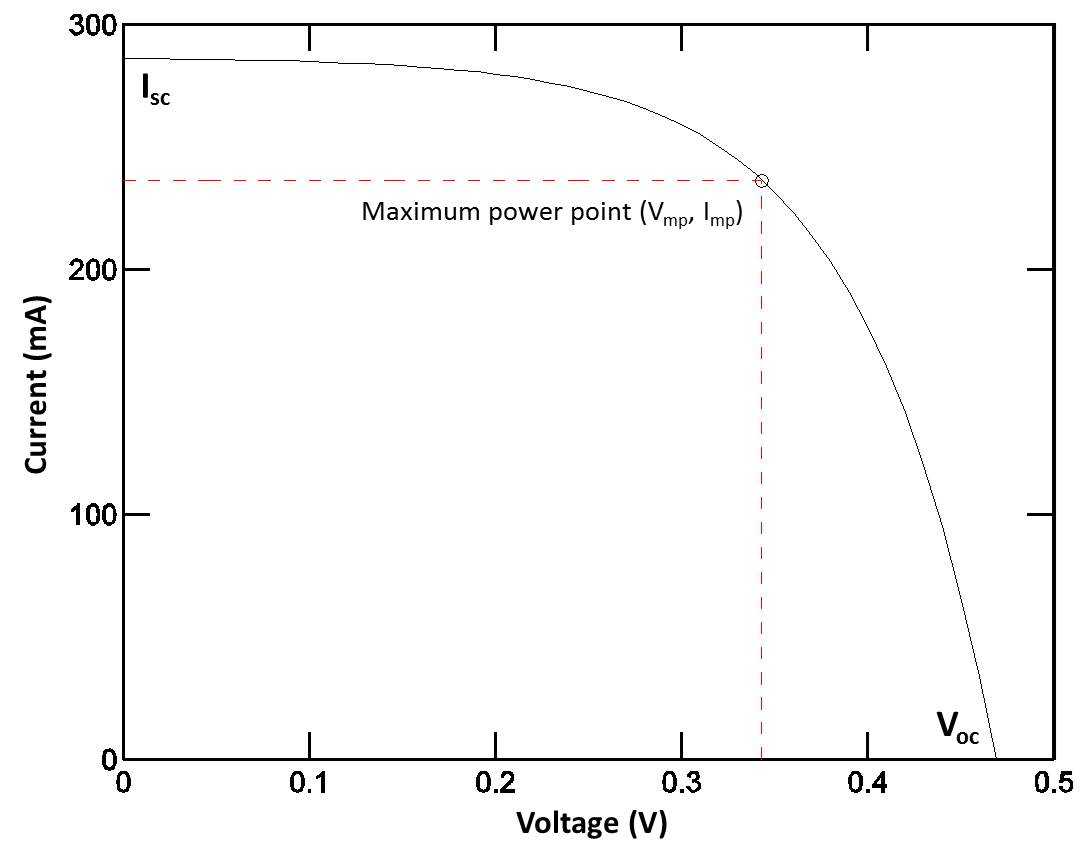
\includegraphics[scale=0.5]{IV.jpg}
\caption{I-V characteristics}
\label{ivcharac}
\end{figure}


The fill factor (FF) and power conversion efficiency ($\eta$) are often represented the solar cell performance:

\begin{equation}
FF=\frac{P_{out}}{V_{oc} \cdot I_{sc}} = \frac{V_{mp} \cdot I_{mp}}{V_{oc} \cdot I_{sc}}
\end{equation}

\begin{equation}
\eta =\frac{P_{out}}{P_{in}} = \frac{FF \cdot V_{oc} \cdot I_{sc}}{P_{in}}
\end{equation}

where $P_{in}$ is the incident photon energy per second. The conversion efficiency of the solar cells is proportional to fill factor, $V_{oc}$, and $I_{sc}$. There are several aspects which will affect
the conversion efficiency. $V_{oc}$ is directly proportional to the band gap of the material, $I_{sc}$ is proportional to the number of absorbed photons. When the band gap is decreased, the more of the spectrum is absorbed, however, 
the $V_{oc}$ will be reduced in this case. On the material surface, the photons are absorbed and recombined, this is severely reduce the efficiency. There is more detailed analysis of conversion efficiency in the Ref[?? Principles of solar energy conversion].


\section{Solar cell materials}

In 1839,  French physicist A. E. Becquerel revealed the photovoltaic effect for the first time, later Charles Fritts built the first solid state photovoltaic (PV) cell using semiconductor selenium in 1883.
It is not until 1941 that the first silicon-based solar cell is demonstrated. Until now, there are many different solar cell materials. The reason why 
best solar cell material do not come out yet is that it is expected to be not only high efficiency but also environmentally friendly and 
low cost. It means that it requires not only that the process of growth and manufacturing solar cell materials should be cheapter, but also that it has longer application life, and the raw material should be abundant and non-toxic as well. In this section,
five main solar cell materials are discussed briefly, that is, silicon (Si), gallium arsenide (GaAs), cadmium telluride (CdTe), Copper indium gallium selenide (Cu(In, Ga)Se\textsubscript{2}).

Potential solar cell materials need to fullfil several properties, such as large absorption coefficient and the range of band gap is around 1 to 1.6 eV. Under these conditions, there 
are quite many materials satisfying the requirements. However, some other properties are needed to be considered as well, such as cost, enviromental safety
and many others. Thereby, only some of them is suitable to produce in reality. In the \textbf{Fig. \ref{lscm}}, evolution for several solar cell materials is illustrated. 

\begin{figure}[H]
\centering
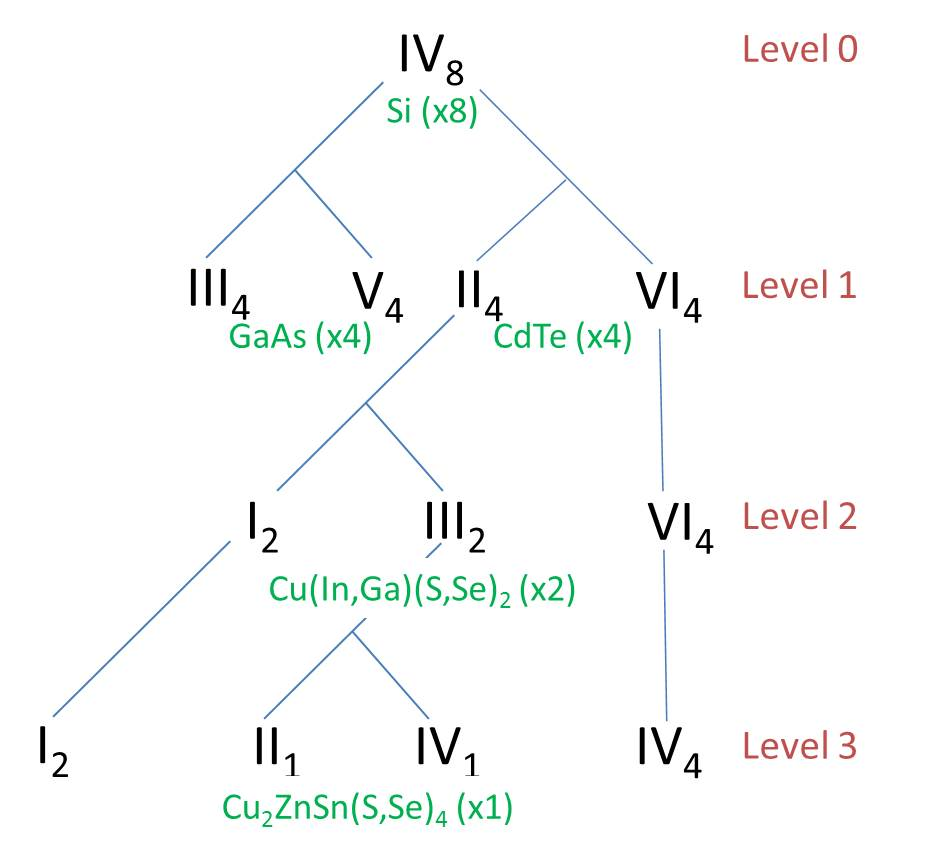
\includegraphics[scale=0.5]{tree.jpg} 
\caption{Tree of tetragonal bonded semiconductor, the roman numerals means the group numbers in the chemical element periodic table, the subscript means the number of elements.}
\label{lscm}
\end{figure}

From above \textbf{Fig. \ref{lscm}}, based on group number IV element silicon (level 0) in the chemistry element periodic table, two categories semiconductor materials are deduced (level 1), such as gallium arsenide (GaAs) in group III-V and cadmium telluride (CdTe)
in group II-VI. The element in group II in level 1 could be further divided into elements in group I and III, such as CIGS and CIGSe (level 2). From the group III in level 2, the element is possible to
be substituted from group II and IV in level 3, such as CZTS and CZTSe.


\subsection{Crystalline silicon solar cells}
The solar cell based on silicon dominates the solar power world currently, which accounts for more than 90\% of the total PV market.
This kind of solar cell takes advantage of different forms of silicon, that is, monocrystalline silicon and polycrystalline silicon. 
The success of Si is due to a number of reasons. In the crust of Earch, there are over 90\% is composed of silicate minerals, which also means huge available amonuts of Si. Moreover, it has higher conversion efficiency, and it is also proved that 
it has excellent stability and reliability under the outdoor condition. However, Si also have drawbacks. It has an indirect band gap and hence it has a lower optical absorption coefficient. In order to absorb the incident sunlight fully, 
it requires to thicker Si to absorb the sunlight. Crystalline Silicon have to be high quality and defect free in order to avoid losting the carriers before collection. Last but not least, it is costy to purify the Si from silicate minerals, which
really limits the cost reduction potential of wafer-based silcion technology. 

However, the solar cells based crystalline silicon technology is still leading the market of solar cell since many companies are trying to lower the cost of the whole process.



\subsection{Gallium arsenide}
Gallium arsenide (GaAs) is a III-V compound of the elements gallium and arsenic. It has a zinc blende crystal structure with a direct bandgap around 1.42 eV. Some electronic properties of GaAs are superior to Silicon, such as higher electron 
mobility, higher saturated electron velocity, absorb sunlight more efficiently due to the direct bandgap. The optimum bandgap for the single junction solar cell is suggested around 1.4 eV by theoretical calculations,
therefore one of the most applications of GaAs is solar cells. GaAs has been extensively researched since the 1950s, and the first GaAs solar cells were established in 1970 by the Zhores Alferov's team. Today,
the conversion efficiency for single function solar cell based on GaAs is around 28.8\%. However, it is more difficult to grow and has higher price compared to Si. Many researches is focusing on how to reduce the price, and 
the main application solar cell based on GaAs is in the space application. At last, the arsenic toxicity is considered as well. 

Recently, the multi-junction solar cells are based on the III-V compounds, and the conversion efficiency record is reached around 37.7\% for multi-junction
device based on InGaP-GaAs-InGaAs lead by the group Sharp.

\subsection{Thin film materials}

Thin film solar cells have several thin films with the total thickness less than \SI{10} {\micro\meter}. The cost can potentially be lower since the less materials are used to make thin film solar cells. The development of thin film
solar cell was started since 1970s. Currently, the conversion efficiency for the single junction already surpassed 20\%, even though it is still not as high as the solar cells based on crystalline silicon. There are mainly four 
thin film materials are considered in the solar cells: amorphous silicon (a-Si), cadmium telluride (CdTe), $\mathbf {Cu(In, Ga)Se_2}$ (CIGS),  and $\mathbf {Cu_{2}ZnSn(S,Se)_{4}}$ (CZTSSe).

Amorphous silcion solar cells are the first thin film solar cell material which reach the large-scale production. It has higher absorption coefficient than crystalline silicion, therefore, the thickness can be less than \SI{1} {\micro\meter}. The 
main disadvantages a-Si solar cells is the lower efficiency, the actual conversion efficiency for the commericial single junction solar cells based on a-Si is between 4\% to 8\%. This limits the development of a-Si thin film solar cells.
A-Si solar cells are suited to the situation which requires low cost over high efficiency. 

CdTe was first reported in the 1960s. However, it is not developed rapidly until in the early 1990s. CdTe has a number of advantages as an absorber. It has higher absorption coefficient. The band gap is around 1.45 eV, which 
is very near the optimum value for single-junction solar cells. Moreover, the process
of manufacturing is easy to control, which means the cost of manufacturing is low. Moreover, the commercial modules already reach the efficiency of 16\%. However, an important question is needed to be considered in order to large-scale CdTe
manufacturing: cadmium toxicity and tellurium availability. 

CIGS are direct band gap seciconductor with high optical absorption coefficients. It is seen as the most promising solar cell material for the near future. It is always used in a heterojunction structure, mainly it is with the thinner
n-type cadmium sulfide layer. The conversion efficiency of CIGS reached up to 20\% in the laboratory cell. The intersting part is that it can be alloyed with Gallium (Ga), and the band gap can be tuned along with that. The band gap 
is between 1 eV to 1.7 eV for this alloy. CIGS does not contain any toxic element. However, the cost and scarcity of Indium (In) will become the major problem for the CIGS.


\section{CIGS materials}
CIGS material is a chalcopyrite-type material, which is considered to be the most promising thin film solar cell material. It has a direct band gap between 1 ev and 1.7 eV,  and the conversion efficiency in laboratory already surpassed 20\%. 
$\mathbf {CuInSe_{2}}$ was first synthesized by Hahn in 1953. It was first used as an absorber material in a single crystal solar cell in 1974, which is based on $\mathbf {CuInSe_{2}}$ and CdS. The conversion efficiency is around 
5\%. The first thin film solar cells based on $\mathbf {CuInSe_{2}}$ and CdS was invented by Kazmerski. During 1980s, Boeing Corporation did much reseach on the thin film polycrystalline CIGS solar cells. 
To date, the highest conversion efficiency in lab situation for the solar cells based on CIGS is between 20\% and 21\% by alloying Ga.


\subsection{Crystal structure}
From the \textbf{Fig. \ref{lscm}}, the crystal structure of CIGS can be derived from the zinc blende crystal structure of ZnSe. In the \textbf{Fig. \ref{crystal_cigs}}, the crystal structure of ZnSe and CIGS is presented. 
The elements Zn are replaced by Cu and In or Ga elements in the zinc blende of ZnSe. It requires to double the unice cell in the z-direction. Because the different bond strength and lengths between
Cu-Se and In-Se or Ga-Se, therefore, the lattice parameter c is not exact 2a normally.

Chalcopyrite CIGS (with x = 0.0 and 1.0) has the space group XYZ (XYZ; space group no. XYZ).
The conventional unit cell has four copper atoms on the Wyckoff positions XYZ, four indium/gallium atoms on position XYZ, and eight selenium atoms on the XYZ position. 
The cation positions have all XYZxyz point-group symmetry, and Se have XYZxyz symmetry. 
The Se XYZxyz position is fully defined with the position (x, y, z), and each anion Se-atom has two inequivalent bonds $\delta$X–Se to the cations X = Cu and In/Ga. 
For the alloy of CIGS (in this work, x = 0.5 with 50\% In and 50\% Ga), the structure is chosen so that each Se atom bonds to two Cu atoms, one In and one Ga atom;
this is the most probable local atomic configuration in a random alloy structure.


\begin{figure}[H]
\centering
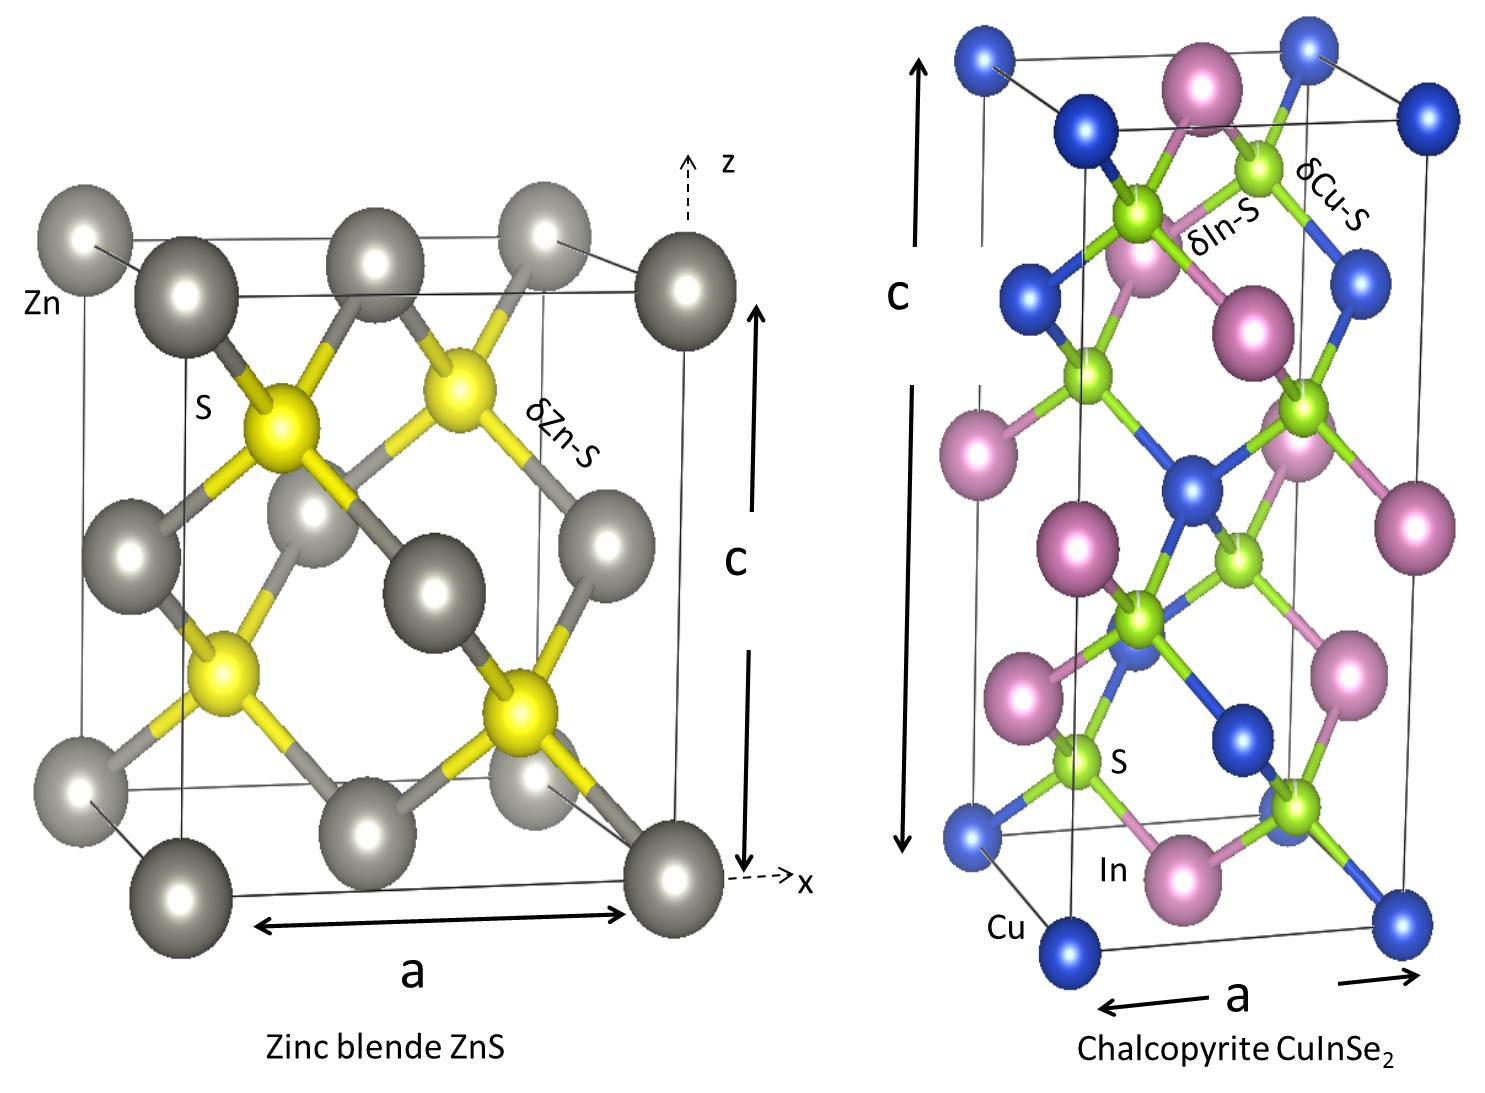
\includegraphics[scale=0.4]{structureciise1.jpg} 
\caption{}
\label{crystal_cigs}
\end{figure}






\subsection{Optical properties and doping in the CIGS}
$\mathbf {CuInSe_{2}}$ has a direct band gap around 1 eV, and the absorption coefficient is above $1 \times 10^{4} cm^{-1}$. The quaternary CIGS alloy will be available by alloying Ga element, while the band gap is tuned as well from 
1.0 eV to 1.7 eV. The high absorption coefficient makes the CIGS material possible to be an absorber for the thin film solar cells. The band gap can be approximated by the function of Ga content (x):

\begin{equation}
E_g(x) = 1.0 + 0.564x+0.116x^2 ??
\end{equation}

Alloying the Ga element will decrease the electron affinity of CIGS, which will make the conduction band upward shift, however, the valence band remain the same postion. This also explains the reason why the band gap increases with 
more Ga element in the CIGS materail. The best solar cell is with the Ga content of 30\% (x=0.3), however, the band gap energy of the CIGS suggests that the optimum solar cell conversion efficiency is obtained with between x=0.5 
and x=0.7. The reason will be discussed in the next paragraph. At last, the overview properties of CIGS material is described in the table ???


CIGS is a nonstoichiometric compound with the deviations from stoichiometry in several pencentage range. The high quality thin film solar cells mainly use Cu-poor (Cu: 22.5-24.5\%) high offstoichiometric CIGS absorber.
The main native defects in CIGS include <2V\textsubscript{Cu}, In\textsubscript{Cu}>, <Cu\textsubscript{In}, In\textsubscript{Cu}>, V\textsubscript{Cu}, In\textsubscript{Cu}, Cu\textsubscript{In} V\textsubscript{Se}
and Ga\textsubscript{Cu}. V\textsubscript{Cu} and III\textsubscript{Cu} are important native defects in CIGS due to
their low formation energies. Therefore, CIGS can be grown p-type easily with the condition of Cu-poor (V\textsubscript{Cu}).

There are some extrinsic divalent cation donors as well, such as Zn\textsubscript{Cu}, Cd\textsubscript{Cu} and Cl\textsubscript{Se}. And the formation energy is relatively low for CIS and CGS. Therefore, it is possible to grow n-type for them.

CIS can be grown n-type under the condition Se-poor or In-rich. However, CGS is not possible to be n-type under equilibrium conditions, because the low formation energy of V\textsubscript{Cu} limits the possibility of achieving electronic n-type character, especially in Ga-rich CIGS.
It is maybe also explained that the Ga-rich CIGS is not suitable for high efficiency solar cells. 


\subsection{CIGS solar cell structure}

The solar cells device based on CIGS is a heterojunction device, which has several thin film layers with different functional properties. A schematic of a conventional device structure is shown in  \textbf{Fig. \ref{device}}

\begin{figure}[H]
\centering
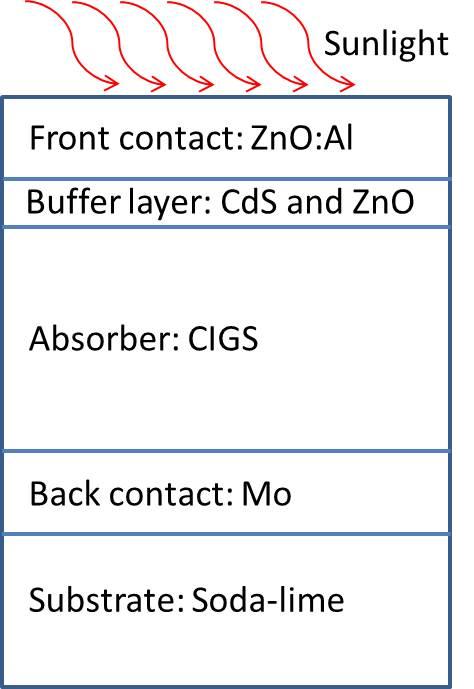
\includegraphics[scale=0.5]{devicestruc.jpg} 
\caption{}
\label{device}
\end{figure}

Substract is on the bottom, and there are mainly three kinds of substract: soda-lime glass, metal and polyimide. The most common substrate is the one based on soda-lime glass with thickness \SI{1} {\mm} to \SI{3} {\mm}. The molybdenum works as back contact due to its low resistivity and stability at high 
temperature with thickness around \SI{500} {\nm}. The most important part of the device is the p-type absorber layer: CIGS, and it is dopped by intrinsic defects. The n-type buffer layer cadmium sulfide (CdS) is on the top of CIGS.
The intrinsic zinc oxide (i-ZnO) and n-type ZnO layer are followed, and it works as window layer. The n-type ZnO is dopped by the aluminum (Al). This CIGS/CdS/ZnO strucutrure was found to improve the cell performance.







\chapter{Theory}

\section{Electronic structure calculations }
\label{ch:dft}

\subsection{The quantum many-body problem}
\label{ch:mb}

\noindent A solid material contains a huge number of atoms (around $10^{23}/cm^3$), and the atom is constructed by nuclei and electrons. 
According to the quantum mechanics principles, all the properties of any system are known if one can figure out a way to solve 
the quantum many-body Schrödinger equation exactly. Let us start from the time-independent many-body Schrödinger equation,

\begin{equation}\label{ssth}
 {\hath} {\wf} = {E} {\wf},
\end{equation}

where $\wf$  is the exact wavefunction for the above Schrödinger equation, $\textbf{r}_\textit{i}$ and $\textbf{R}_\textit{I}$  stands for electron and
nucleus coordinators, respectively.

In the Eq. \ref{ssth}, $E$ is the total energy of the system, and $\hath$ is the Hamiltonian which has the following form:

\begin{equation}\label{th}
\begin{split}
& \hath = - \sumi<i> {\frac{\hbar^{2}}{2 m_{\textit e}}}   \nablaia<i> - \sumi<I> {\frac{\hbar^{2}}{2 M_\textit{I}}} \nablaia<I>  - \sumij<i><I> \frac{Z_\textit{I}\ e^2}{4 \pi \varepsilon_0 |\textbf{r}_\textit{i}-\textbf{R}_\textit{I}|} \\
& + \frac{1}{2} \suminj<i><j> \frac{ e^2}{4 \pi \varepsilon_0 |\textbf{r}_\textit{i}-\textbf{r}_\textit{j}|} + \frac{1}{2} \suminj<I><J> \frac{Z_\textit{I} Z_\textit{J}\  e^2}{4 \pi \varepsilon_0 |\textbf{R}_\textit{I}-\textbf{R}_\textit{J}|},
\end{split}
\end{equation}

where the indices $\textit{i}$, $\textit{j}$ are used for electron and $\textit{I}$, $\textit{J}$ are used for atomic nuclei, $Z_\textit{I}$ means the charge of the $\textit{I}$-th nucleus,
$\textit{M}$ denotes the nuclear mass, $m_e$ is the electron mass, $\varepsilon_0$ is vacuum permittivity.

In atomic units, the reduced Planck constant $\hbar$, the electron mass $m$, the Bohr radius $a_0$, and the electron charge
$e$ are equal to 1. The Bohr radius is given by the formula $a_0$ = ${\hbar} / {(mc\alpha)}$, where $\alpha$ is the fine structure
constant ($\alpha$ = ${e^2}/{(4 \pi \varepsilon_0 c \hbar)}$) , so the velocity of light in atomic units is $c$ = $1/{\alpha}$ and ${e^2}/{(4 \pi \varepsilon_0)}$= 1. The Schrödinger Eq. (\ref{th}) in atomic units has 
the following form:

\begin{equation}\label{sth}\begin{split}
&\hath = - \sumi<i>   \frac{{{\nabla}_{\textit{i}}^{2}}}{2} - \sumi<I> \frac{{{\nabla}_{\textit{I}}^{2}}}{2 M_\textit{I}}  - \sumij<i><I> \frac{Z_\textit{I}}{|\textbf{r}_\textit{i}-\textbf{R}_\textit{I}|} \\
& + \frac{1}{2} \suminj<i><j> \frac{1}{ |\textbf{r}_\textit{i}-\textbf{r}_\textit{j}|} + \frac{1}{2} \suminj<I><J> \frac{Z_\textit{I} Z_\textit{J}\ }{|\textbf{R}_\textit{I}-\textbf{R}_\textit{J}|}.
\end{split}\end{equation}

In Eq. \ref{sth}, the first and second terms are the kinetic energy operator of the electron and nuclei, respectively.
The other terms in order are Coulomb interactions between electrons and nuclei, electrons and electrons and nuclei and nuclei.

Since there are so many atoms to calculate in reality, more importantly, the exactly form of the wavefunction is unknown,
so one can not solve the Eq. \ref{ssth} exactly at present. To approximate the exact solution, 
generally one can divide it into three different levels, the first level is the Born-Oppenheimer approximation and the second level is Hartree,
Hartree-Fock (HF), density functional theory (DFT) and Kohn-Sham (KS) equation, and the last level is to solve the secular equation, 
which is an equation that is solved to find the eigenvalue of matrix.

\subsection{The Born-Oppenheimer approximation}
\label{ch:boa}

In order to simplify the Eq. \ref{ssth}, the first attempt is to seperate the wavefunction of electrons and nuclei, but since there is a couple term between the electron and nucleus in the Schrödinger Hamitonian in Eq. (\ref{sth}), 
thereby one can not do that simply. On the other hand, let us observe the Eq. \ref{sth} again, there exists a small value ${1}/{M_I}$, which is part of the nucleus kinetic energy
operator term, the reason is that the mass of nucleus is much larger than that of electron, so the nuclei are treated as fixed. The result is that the electrons is seen as interacting under both the external potential caused by nuclei that are fixed in 
some positions and that of the other electrons. A more vividly description is seen from \textbf{Fig. \ref{figbo}}:

\begin{figure}[H]
\centering
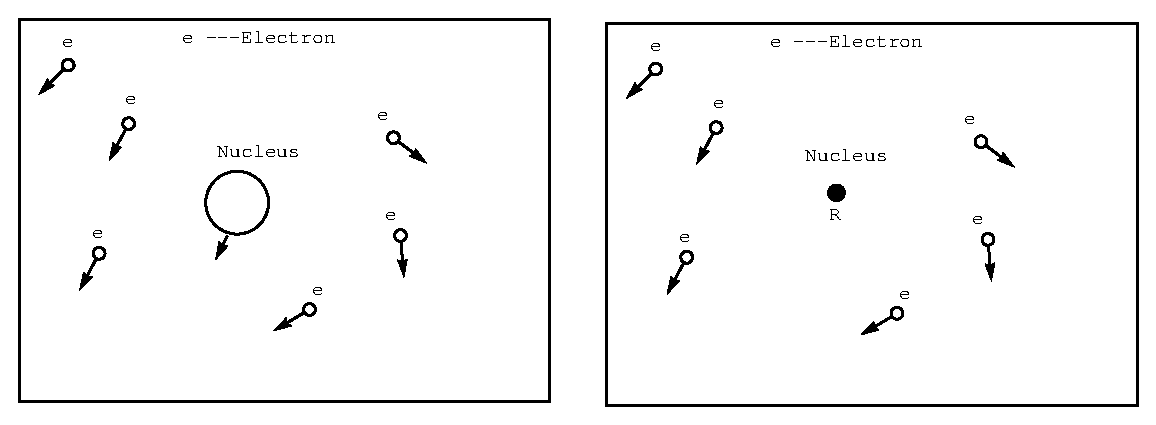
\includegraphics[scale=.7]{system.eps}
\caption{Left panel: normal interacting system. Right panel: the Born-Oppenheimer approximation. The arrows denotes the movement of the nucleus or electron.}
\label{figbo}
\end{figure}

The separation of motion between electrons and nuclei is called the Born-Oppenheimer approximation, since the position of nuclei is fixed, one can define:

\begin{equation}\label{nwf}
{\wf}  {\approx}  {\Psi_{ \textit{BO}} ( \{ {\textbf{r}_{\textit{i}}},\textbf{R}_{\textit I} \}) } = {\theta(\{{\textbf R}_{\textit I}\})} {\Psi'(\{\textbf{r}_{\textit i}\}; \{{\textbf R}_{\textit I}\})},
\end{equation}

where ${\Psi'(\{\textbf{r}_{\textit i}\}; \{{\textbf R}_{\textit I}\})}$  is the electrons wavefunction in the Born-Oppenheimer approximation, the semicolon means that $\textbf R_I$ is only discrete value belonging to the set of atomic positions. 
 
The Eq. \ref{sth} can be defined as:

\begin{equation}\label{nh}
 {\hath} = - \sumi<I> \frac{{{\nabla}_{\textit{I}}^{2}}}{2 M_\textit{I}} + {\hath}_{BO}.
\end{equation}

where 

\begin{equation}\label{both}\begin{split}
&{\hath}_\textit{BO}\ =\ - \sumi<i>   \frac{{{\nabla}_{\textit{i}}^{2}}}{2}  - \sumi<i> V_{ext}(\textbf{r}_{\textit{i}})  + \frac{1}{2} \suminj<i><j> \frac{1}{ |\textbf{r}_\textit{i}-\textbf{r}_\textit{j}|} + \frac{1}{2} \suminj<I><J> \frac{Z_\textit{I} Z_\textit{J}\ }{|\textbf{R}_\textit{I}-\textbf{R}_\textit{J}|} \\
&\ = \ \hat{T} \ + \ \hat{V}_{ext} \ + \ \hat{V}_\textit{int}\ + \ N_\textit{II},
\end{split}\end{equation}

and

\begin{equation}\label{vext}
V_{ext}(\textbf{r}_{\textit{i}}) =  \sumi<I> \frac{Z_\textit{I}}{|\textbf{r}_\textit{i}-\textbf{R}_\textit{I}|},
\end{equation}

where ${\hath}_\textit{BO}$  is the Hamitonian for the electrons within the Born-Oppenheimer approximation. The subscript $ext$ means $external$ in Eq. \ref{vext}, this term describes the external potentials interaction. 

Thereby, the new Schrödinger equation with Eq. \ref{nwf} and Eq. \ref{nh} is 

\begin{equation}
 (- \sumi<I> \frac{{{\nabla}_{\textit{I}}^{2}}}{2 M_\textit{I}} + {\hath}_{BO} ) ({\theta(\{{\textbf R}_{\textit I}\})} {\Psi'(\{\textbf{r}_{\textit i}\}; \{{\textbf R}_{\textit I}\})}) = E_{m}(\{{\textbf R_I}\}) ({\theta(\{{\textbf R}_{\textit I}\})} {\Psi'(\{\textbf{r}_{\textit i}\}; \{{\textbf R}_{\textit I}\})}).
\end{equation}
 
\noindent Here, $E_{m}(\{{\textbf R_I}\})$ is the total energy, after some steps of derivation, one can end up with the Eq. \ref{bose} :

\begin{equation}\label{bose}
{\hath}_{BO} {\Psi'(\{\textbf{r}_{\textit i}\}; \{{\textbf R}_{\textit I}\})} = E_\textit{BO}{(\{\textbf{R}_{\textit I}\})} {\Psi'(\{\textbf{r}_{\textit i}\}; \{{\textbf R}_{\textit I}\})},
\end{equation}

\noindent where $E_\textit{BO}{(\{\textbf{R}_{\textit I}\})}$ is the energy of this electronic system,

\begin{equation}\label{ise}
( \hat{H}_{I1}+\hat{H}_{I2}+\hat{H}_{I3}+E_{BO}(\{{\textbf R}_{\textit I}\}) ) {\theta(\{\textbf{R}_{\textit I}\})} = E_{m}(\{{\textbf R_I}\}) {\theta(\{\textbf{R}_{\textit I}\})},
\end{equation}

where

\begin{equation}\begin{split}
 &  \hat{H}_{I1} = - \sumi<I> \frac{{{\nabla}_{\textit{I}}^{2}}}{2 M_\textit{I}}   \\
 &  \hat{H}_{I2} = - \sumi<I> \frac{1}{M_\textit{I}} {\int {\Psi'(\{\textbf{r}_{\textit{i}}\}; \{\textbf{R}_{\textit I}\})}^{\ast} {{\nabla}_{\textit{I}}} {{\Psi'(\{\textbf{r}_{\textit{i}} \}; \{\textbf{R}_{\textit I}\})}} d {\textbf r }} {{\nabla}_{\textit{I}}}  \\
 &  \hat{H}_{I3} = - \sumi<I> \frac{1}{M_\textit{I}} {\int {{\Psi'(\{\textbf{r}_{\textit{i}}\}; \{\textbf{R}_{\textit I}\})}}^{\ast} {{\nabla}_{\textit{I}}^{2}} {{\Psi'(\{\textbf{r}_{\textit{i}} \}; \{\textbf{R}_{\textit I}\})}} d {\textbf r }}. 
\end{split}\end{equation}

From Eq. \ref{ise}, one observes that the lattice dynamical properties of certain system within the Born-Oppenheimer approximation could be obtained. To solve this equation,
the ground state energy $E_{BO}(\{{{\textbf R}_{\textit I}}\})$ of electron system is needed. Here $\{{\textbf R}_{\textit I}\}$ are the parametrilized values from the atom position.
 
In summary, the Schrödinger equation of electron and nucleus is derived seperately within the Born-Oppenheimer approximation. When one refers to calculations of the ground state properties,
which means to take use of the Schrödinger equation of electron only, e.g., Eq. \ref{bose}, and Schrödinger equation of nucleus is used for the calculation of lattice dynamics.

One notices that the Eq. \ref{both} is much simpler than Eq. \ref{sth}, but still the equation is not solvable. Further approximations  are needed
to solve this many-body problem.

\subsection{Hartree, Hartree-Fock approximation and density functional theory}

From last section, the seperation of wavefunction is given within Born-Oppenheimer approximation, the quantum many-body Schrödinger problem becomes the many-electron 
Schrödinger problem. There are two major problems from the Born-Oppenheimer approximation, the first problem is that the number of electron is around $10^{23}/cm^3$, it is a huge numerical problem, however, it is still possible to solve.
The second one is that the Hamiltonian operator is applied to single electron, however, the wavefunction is not shown how it depends on the single-electron wavefunction. The latter problem 
could be solved by the following three methods:

The first method is to figure out a way to seperate or approximate the wavefunction into single-electron function, like the Hartree and Hartree-Fock (HF) method. The second method is to
find a Hamiltonian which is possbile to act on wavefunction directly, like density functional theory (DFT). Either of these two methods has "pros and cons". The third one is called Kohn-Sham equation,
which is a combination of above two methods. It starts from DFT, but takes advantage of single-electron wavefunction. This will be demonstated in the next section.

\subsubsection{Hartree approximation}
\label{ha}
The simplest approximation of the wavefunction for the many-electron Schrödinger equation is the form of acting like independent
electrons, the wavefunction with N independent electrons has the following expression:

\begin{equation}\label{wfh}
\wfh = \bwf<1><1> \bwf<2><2> \cdots \bwf<N><N>, 
\end{equation}

where $i$ goes through all the electrons, and  means state of the $i$-th electron in the position of ${\textbf{r}}_{\textit{i}}$, 
from here and following the $\textbf R$ is suppressed in the wavefunction since they are in fixed position. The total energy of the system can be written down 
in the following way :

\begin{equation}\label{teh}
E_{\textit{H}} = <\wfh |\ {\hath}_{\textit{BO}} \ | \wfh  >.
\end{equation}

Therefore, making the substitution using Eq. \ref{both} and \ref{wfh} into Eq. \ref{teh}, the total energy of system is:
\begin{equation}\begin{split}
&E_\textit{H} = \sumi<i> <\bwf<i><> |\ -\frac{\nabla^{2}_{i}}{2} + V_\textit{ext}(\textbf{r})  \ | \bwf<i><> > \\
& +\frac{1}{2} \suminj<i><j> <\bwf<i><> \bwfn<j><'>|\ \frac{1}{|\textbf{r} - \textbf{r}^{'} |} \ | \bwf<i><> \bwfn<j><'>>.
\end{split}\end{equation}

In order to calculate the stationary state with the lowest energy of the system, the variation of the wavefunction should be
zero variation in the energy, one can set up the following equation with Lagrange multiplier $E^{i}_H$,

\begin{equation}\label{haa}
 \delta [ E_{\textit{H}} - \sumi<i> E^{i}_{H} (<\bwf<i><> | \bwf<i><> > -1)] = 0. 
\end{equation}

where $(<\bwf<i><> | \bwf<i><> > -1)$ means that the wavefunction is normalized.

In order to calculate the term $\delta ( E_{\textit{H}} ) $, one has to derive

\begin{equation}\begin{split}\label{hartree1}
& \delta ( \sumi<i> <\bwf<i><> |\ -\frac{\nabla^{2}_{ i}}{2} + V_\textit{ext}(\textbf{r})  \ | \bwf<i><> > ) \\
&  = \sumi<i> \{ < \delta \bwf<i><> |\ -\frac{\nabla^{2}_{i}}{2} + V_\textit{ext}(\textbf{r})  \ | \bwf<i><> >  \\
&  + <  \delta \bwf<i><> |\ -\frac{\nabla^{2}_{i}}{2} + V_\textit{ext}(\textbf{r})  \ |  \bwf<i><> >^{\ast} \}.
\end{split}\end{equation}

and 

\begin{equation}\begin{split}\label{hartree2}
&  \delta( \frac{1}{2} \suminj<i><j> <\bwf<i><> \bwfn<j><'>|\ \frac{1}{|\textbf{r} - \textbf{r}^{'} |} \ | \bwf<i><> \bwfn<j><'>>)   \\
& =   \frac{1}{2} \suminj<i><j> \{  <\delta \bwf<i><> \bwfn<j><'>|\ \frac{1}{|\textbf{r} - \textbf{r}^{'} |} \ | \bwf<i><> \bwfn<j><'>>  \\
& +   < \bwf<i><> \delta \bwfn<j><'>|\ \frac{1}{|\textbf{r} - \textbf{r}^{'} |} \ | \bwf<i><> \bwfn<j><'>> +  T_{rem}\},
\end{split}\end{equation}

where $T_{rem}$ is the remaining terms, actually these remaining terms will not affect the derivation.

Before getting the final result, there is one more identity 

\begin{equation}\begin{split}\label{hartreelabel1}
& < \bwf<i><> \delta \bwfn<j><'>|\ \frac{1}{|\textbf{r} - \textbf{r}^{'} |} \ | \bwf<i><> \bwfn<j><'>> \\
& = \int d \textbf{r} d \textbf{r}{'}  \phi_{i}^{*} (\textbf{r}{}) \delta \phi_{j}^{*} (\textbf{r}{'}) \frac{1}{|\textbf{r} - \textbf{r}^{'} |}  \phi_{i}^{} (\textbf{r}{})  \phi_{j}^{} (\textbf{r}{'})\\
& = \int d \textbf{r}{'} d \textbf{r}  \phi_{i}^{*} (\textbf{r}{'}) \delta \phi_{j}^{*} (\textbf{r}{}) \frac{1}{|\textbf{r}{'} - \textbf{r} |}  \phi_{i}^{} (\textbf{r}{'})  \phi_{j}^{} (\textbf{r})\\
& = <\delta \bwf<j><> \bwfn<i><'>|\ \frac{1}{|\textbf{r} - \textbf{r}^{'} |} \ | \bwf<j><> \bwfn<i><'>>.
\end{split}\end{equation}

\noindent So the Eq. \ref{hartree2} will become 

\begin{equation}\begin{split}\label{hartree3}
&  \delta( \frac{1}{2} \suminj<i><j> <\bwf<i><> \bwfn<j><'>|\ \frac{1}{|\textbf{r} - \textbf{r}^{'} |} \ | \bwf<i><> \bwfn<j><'>>)   \\
& =  \suminj<i><j> \{  <\delta \bwf<i><> \bwfn<j><'>|\ \frac{1}{|\textbf{r} - \textbf{r}^{'} |} \ | \bwf<i><> \bwfn<j><'>> + \frac{T_{rem}}{2}\}.
\end{split}\end{equation}


Taking use of the above two Eq. \ref{hartree1}, \ref{hartree3} and variation in the term of  $\delta \phi^{*}_{i}(\textbf{r}{}) $, the Eq. \ref{haa} becomes:

\begin{equation}
\begin{split}\label{hha}
& \frac{1}{\delta  \phi^{*}_{i}(\textbf{r}{})} \delta [ E_{\textit{H}} - \sumi<i> E^{i}_{H} (<\bwf<i><> | \bwf<i><> > -1)] \\
&  = \frac{1}{\delta  \phi^{*}_{i}(\textbf{r}{})} \{ \sumi<i> \{ < \delta \bwf<i><> |\ -\frac{\nabla^{2}_{i}}{2} + V_\textit{ext}(\textbf{r})  \ | \bwf<i><> > + <  \delta \bwf<i><> |\ -\frac{\nabla^{2}_{i}}{2} + V_\textit{ext}(\textbf{r})  \ |  \bwf<i><> >^{\ast} \} \\
& +  \suminj<i><j> \{  <\delta \bwf<i><> \bwfn<j><'>|\ \frac{1}{|\textbf{r} - \textbf{r}^{'} |} \ | \bwf<i><> \bwfn<j><'>> + \frac{T_{rem}}{2}\} - \sumi<i> E^{i}_{H} (<\bwf<i><> | \bwf<i><> > -1) \} \\
& =  { \{-\frac{\nabla^{2}_{i}}{2} + V_\textit{ext}(\textbf{r})} \}  \bwf<i><> +  \suminj<j><i> \{  <\bwfn<j><'>|\ \frac{1}{|\textbf{r} - \textbf{r}^{'} |} \ | \bwf<i><> \bwfn<j><'>> - E^{i}_{H}  \bwf<i><>  \}.
\end{split}
\end{equation}

Therefore,
\begin{equation}
(-\frac{\nabla^{2}_{i}}{2} + V_\textit{ext}(\textbf{r})+ \suminj<j><i> <\bwfn<j><'>\ | \frac{1}{|\textbf{r} - \textbf{r}^{'} |} \ | \bwfn<j><'>>) \bwf<i><> = E^{i}_{H} \bwf<i><>,
\end{equation}

where $E^{i}_{H}$  also can be treated as the energy. The Eq. \ref{hha} is a group of dependent single
 particle equations, and after checking it, one will find out this equation is self-consistent and can be solved using iteratively.

\subsubsection{Hartree-Fock approximation}
Hartree approximation is the simplest approximation, and Hartree-Fock approximation is the method which considers the 
antisymmetry of the wavefunction. It means that if the positions of two electrons (with same spin) are exchanged, the wavefunction should change the sign, like:

\begin{equation}\label{hfwf}
\Psi_\textit{HF} ( \cdots \textbf{r}_\textit{i} \cdots  \textbf{r}_\textit{j} ) = - \Psi_\textit{HF} ( \cdots \textbf{r}_\textit{j} \cdots  \textbf{r}_\textit{i} ).
\end{equation}

Slater introduced an way to construct the wavefunction due to the Eq. \ref{hfwf} based on the Hartree approximation, 
the wavefunction of the many-electron Schrödinger equation is described in a matrix determinant for the N number of electrons 
(without spin):

\begin{equation}\label{hfwfm}
\Psi_{HF}(\mathbf{r}_1, \mathbf{r}_2, \ldots, \mathbf{r}_N) =
\frac{1}{\sqrt{N!}} \left|
\begin{matrix}
    \bwf<1><1> & \bwf<1><2> & \cdots & \bwf<1><N> \\
    \bwf<2><1> & \bwf<1><2> & \cdots & \bwf<1><N> \\
    \vdots               & \vdots               &        & \vdots               \\
    \bwf<N><1> & \bwf<N><2> & \cdots & \bwf<N><N>
\end{matrix} \right|,
\end{equation}
\noindent where $i$ goes through all the electron, and $\bwf<i><i>$ means state of the ($i$)-th electron in the position of $\textbf{r}_\textit{i}$, so if one exchanges two columns
 in the Eq. \ref{hfwfm}, the result is satisfied with the Eq. \ref{hfwf}.

Repeating all the processes already done through the Hartree approximation, the total energy of Hartree-Fock is:

\begin{equation}\begin{split}
&E_\textit{HF} = \sumi<i> <\bwf<i><> |\ -\frac{\nabla^{2}_{i}}{2} + V_\textit{ext}(\textbf{r})  \ | \bwf<i><> > \\
& + \frac{1}{2} \suminj<i><j> <\bwf<i><> \bwfn<j><'>|\ \frac{1}{|\textbf{r} - \textbf{r}^{'} |} \ | \bwf<i><> \bwfn<j><'>> \\
& - \frac{1}{2} \suminj<i><j> <\bwfn<i><'> \bwfn<j><>|\ \frac{1}{|\textbf{r} - \textbf{r}^{'} |} \ | \bwfn<i><> \bwfn<j><'>>.
\end{split}\end{equation}

In the same mathematical way as in previous sectrion but somewhat more complicated, the singe particle Hartree-Fock equation can be obtained:

\begin{equation}\begin{split}
& \{ -\frac{\nabla^{2}_{\textit i}}{2} + V_\textit{ext}(\textbf{r})+ \suminj<j><i> <\bwfn<j><'>\ | \frac{1}{|\textbf{r} - \textbf{r}^{'} |} \ | \bwfn<j><'>> \} \bwf<i><>  \\
& - \suminj<i><j>  < \bwfn<j><'>|\ \frac{1}{|\textbf{r} - \textbf{r}^{'} |} \ | \bwfn<i><'> >) \bwfn<j><>  = E^{i}_{HF} \bwf<i><>.
\end{split}\end{equation}

Compared with Hartree equation, there is an extra term in the equation above. This is called exchange term. In order to organize the equation in a nice and clear way, finally it ends up with:
\begin{equation}\label{aaaaa}\begin{split}
\{ -\frac{\nabla^{2}_{\textit i}}{2} + V_\textit{ext}(\textbf{r}) +V_\textit{H}(\textbf{r}) \}  \bwf<i><>  = E^{i}_{HF}   \bwf<i><>, 
\end{split}\end{equation}
where
\begin{equation}
 V_\textit{H}(\textbf{r})= \int \frac{\rho(\textbf{r}{'}) - \rho_{\textit{i}}^{\textit{HF}}(\textbf{r},\textbf{r}{'})}{|\textbf{r} - \textbf{r}^{'} |}  \mathrm{d}\textbf{r}^{'}.
\end{equation}

\begin{equation}
\begin{split}
& \rho_{\textit{i}}^{\textit{HF}}(\textbf{r},\textbf{r}{'}) = \sumi<j> \frac{\phi_{i}^{}(\textbf{r}{'}) \phi_{i}^{*}(\textbf{r}{}) \phi_{j}^{}(\textbf{r}{}) \phi_{j}^{*}(\textbf{r}{'})} {\phi_{i}^{}(\textbf{r}) \phi_{i}^{*}(\textbf{r})}  \\
& \rho(\textbf{r}) = \sumi<i>  {|\bwf<i><>|}^{2}.
\end{split}
\end{equation}

The Eq. \ref{aaaaa} could be solved in the same way like Hartree approximation but plus one extra term.

\subsubsection{Density functional theory}
The Hartree and Hartree-Fock methods are very classic methods to solve the many-electron 
 Schrödinger equation. However, the HF method only includes the exchange term, not the electron correlation term, they are not suitable in the case of electrons in solid.
 Apart from the two methods mentioned before, there is a modern method to deal with
 the more complicated calculation of electrons, namely, the density functional theory, which is introduced by Hohenberg and
 Kohn in 1964, Kohn and Pople was awarded Chemistry Nobel Prize in 1998.

The idea of the DFT is to treat the electron density of solid instead of using the many-particle wavefunction, so one can
 benefit that the degree of freedom reduces from 3N (N is the number of electrons) to 3, which is apparently less complicate than 
those of Hartree and Hartree-Fock during calculation. 

$\textbf{The density as basic variable}$ 

There are two questions coming out if considering the electron density as the role of wavefunction. The first one is whether it
 is the equivalence relation between the electron density and wavefunction of the system, and the second one is how to solve this 
problem. In order to know that there are two very basic theorems introduced by Hohenberg and Kohn:

\begin{thm}
\label{hk1}
\noindent The first theorem states that the external potential $V_\textit{ext}(\textbf{r})$  is determined uniquely for any electron system by the ground state electron density $\rho$.
\end{thm}

The above theorem also indicate that all the ground state properties are determined by the true ground state density $\rho$,
for example, the total energy E=E[$\rho$]. 

The above theorem also explains the equivalence relation between the electron density and wavefunction, because Hamiltonian is obtained from external potential,
then one can get the wavefunction, therefore the corresponding electron density is determined. Moreover, from the theorem, the external potential is unique decided by electron
density, therefore, the electron density contains the same information as the wavefunction.

The proof of the theorem is following:

Let us assume that there exsits two external potentials named $V^{1}_\textit{ext}(\textbf{r})$ and $V^{2}_\textit{ext}(\textbf{r})$ leading to the same ground state 
electron density $\rho$. Obviously, this will lead to two different Hamiltonians, that is, $\hat{H}_{1}$ and $\hat{H}_{2}$, and as well as two different corresponding
wavefunctions named $\Psi_1$ and $\Psi_2$. Since $\Psi_1$ are not the ground state wavefunction of $\hat{H}_{2}$, the same rules to $\Psi_2$ and $\hat{H}_{1}$, two following
inequality equations will be satisfied:

\begin{equation}\label{hkpf1}\begin{split}
&  E_1 = \langle \Psi_1\ |\hat{H}_{1}|\ \Psi_1 \rangle  \ < \  \langle \Psi_2\ |\hat{H}_{1}|\ \Psi_2 \rangle.\\
&  E_2 = \langle \Psi_2\ |\hat{H}_{2}|\ \Psi_2 \rangle  \ < \  \langle \Psi_1\ |\hat{H}_{2}|\ \Psi_1 \rangle.
\end{split}\end{equation}

Taking advangtage of the form of Hamitonian from Eq. \ref{both}, one can get:
\begin{equation}\label{hkpf2}\begin{split}
&    \langle \Psi_2\ |\hat{H}_{1}|\ \Psi_2 \rangle \\
&  = \langle \Psi_2\ |\hat{H}_{2} + \hat{H}_{1} - \hat{H}_{2}|\ \Psi_2 \rangle \\
&  = \langle \Psi_2\ |\hat{H}_{2} |\Psi_2 \rangle + \langle \Psi_2 | \hat{H}_{1} - \hat{H}_{2}|\ \Psi_2 \rangle \\
&  = E_2 + \int d \textbf{r} ( V^{1}_\textit{ext}(\textbf{r}) - V^{2}_\textit{ext}(\textbf{r}) )  \rho.
\end{split}\end{equation}

Using Eq. \ref{hkpf1} and Eq. \ref{hkpf2}, one can get:

\begin{equation}\label{hkpf3}
 E_1  < \  E_2 + \int d \textbf{r} ( V^{1}_\textit{ext}(\textbf{r}) - V^{2}_\textit{ext}(\textbf{r}) )  \rho.
\end{equation}

Another similar inequality equation will be gained if one changes the form of equation $\langle \Psi_1\ |\hat{H}_{2}|\ \Psi_1 \rangle$ like Eq. \ref{hkpf2}.
\begin{equation}\label{hkpf4}
  E_2  < \  E_1 + \int d \textbf{r} ( V^{2}_\textit{ext}(\textbf{r}) - V^{1}_\textit{ext}(\textbf{r}) )  \rho.
\end{equation}

Plus the left and right sides from Eq. \ref{hkpf3} and \ref{hkpf4}, one will gain a contradictory result:
\begin{equation}\label{hkpf4}
  E_1 + E_2  < \  E_2 + E_1.
\end{equation}

Thereby, The external potential $V_\textit{ext}(\textbf{r})$ is unique.

\begin{thm}
\label{hk2}
\noindent The second theorem states that there is a universal functional $F[\rho]$ for the total energy in the terms of the electron density $\rho$ with any external potential $V_\textit{ext}(\textbf{r})$ ,
and the exact ground state density is gained when the ground state total energy functional reaches its minimal value, that is, E[$\rho'$]>E[$\rho$], where $\rho$ is the exact ground state density.
\end{thm}

The proof of theorem is following:
because of the first theorem, the total energy can be expressed in the following way (ignoring the interaction between nuclei):
\begin{equation}\label{hkpf5}\begin{split}
& E[\rho] \ =\langle \Psi  | \ \hat{T} \ + \ \hat{V}_\textit{int}  \ + \ \hat{V}_\textit{ext} \ | \Psi \rangle \\
&     = \langle \Psi  | \ \hat{V}_\textit{ext} \ | \Psi \rangle  + \underbrace{\langle \Psi  | \ \hat{T} \ + \ \hat{V}_\textit{int}  \ \ | \Psi \rangle}  \\
&     =   \ \int \rho(\textbf{r}) V_\textit{ext}  + \                    F[\rho]. 
\end{split}
\end{equation}

In the above Eq. \ref{hkpf5}, the term of $F[\rho]$ is the universal functional for all the system of electrons.

The functional of total energy $E[\rho']$ reach the minimum at the exact ground state electron density $\rho$:
\begin{equation}\begin{split}
 & E[\rho'] \ =   \ \int \rho'(\textbf{r}) V_\textit{ext}  + \  F[\rho'] > E[\rho]. 
\end{split}
\end{equation}
 


From above equation, one knows the total energy for the case of exact ground state electron density is lower than any other cases, which also means that one can get 
the exact ground state electron density by minimizing the total energy.



From those two theorems, one definitely know how to solve this problem theoretically, but in practice, $E[\rho]$ is unknown. 
Therefore, one more method is needed to deal with it, this is so called Kohn-Sham (KS) equation.

\subsubsection{Kohn-Sham equation}

The Hartree and Hartree-Fock methods are introduced to solve the many-body problem, both of which are based on the idea of transforming complex 
many-electron problem to single-electron problem by using different wavefunction. The DFT only consider to take use of information from Hamitonian, however not solvable. 
Therefore, is it possbile to combine these two ideas together? the answer is yes, the DFT is solved by Kohn-Sham equation introduced by Kohn and Sham in 1965,
which is constructed in the following text (ignoring the interaction between nuclei).

Assume that the exact ground-state density is obtained by the wavefunction $\wfks = \bwf<1><1> \bwf<2><2> \cdots \bwf<M><M>$, where M is a number which is 
less than $10^{23}$ a lot and $\bwf<i><i>$ is auxiliary independent single-electron wavefuntion:

\begin{equation}\label{ks1}
 \rho(\textbf{r}) = \sumi<i> {\phi^{*}_{i}(\textbf{r})} {\phi_{i}(\textbf{r})}.
\end{equation}

If the density is exact, thereby, the total energy is defined exactly, which can be expressed by the following:

\begin{equation}\label{kse}
\begin{split}
&E[\rho] \ =\ T[\rho] \ + \ V_\textit{int}[\rho] \ + \ V_\textit{ext}[\rho]  \\
&\ \ \   = \underbrace{\ (T[\rho] \ - \ T_{0}[\rho]) \ + \  (V_\textit{int}[\rho] \ - \ V_\textit{HF}[\rho])\ }+ \ T_{0}[\rho] \ + \ V_\textit{HF}[\rho] \ + V_\textit{ext}[\rho]       \\
&\ \ \   = \ T_{0}[\rho] \ + \ V_\textit{HF}[\rho] \ + \ V_\textit{C}[\rho] +\ V_\textit{ext}[\rho],
\end{split}
\end{equation}

where $E[\rho]$  is the total energy, $\rho$ is the ground state density. $T[\rho]$, $V_\textit{int}[\rho]$ and $V_\textit{ext}[\rho]$ in order are the energy from external potential, the exact kinetic 
and the exact electron-electron potential energy. $T_{0}[\rho]$ is the kinetic energy of independent electrons, $V_\textit{HF}[\rho]$ is the potential from the Hartree-Fock approximation and $V_\textit{C}[\rho]$
denotes correlation energy.

From the Hartree-Fock approximation, one can further know that:
\begin{equation}
 V_\textit{HF}[\rho] \ = \ V_\textit{H}[\rho] \ + \ V_\textit{X}[\rho], 
\end{equation}

where $V_\textit{H}[\rho]$ and $ V_\textit{X}[\rho] $ are the Hartree contribution and exchange contribution, respectively. Thereby, the Eq. \ref{kse} can be further defined like
 the following:

\begin{equation}\label{ccc}
\begin{split}
&E[\rho]\ = \ T_{0}[\rho] \ + \ V_\textit{H}[\rho] \ + \ V_\textit{ext}[\rho] \ + \ \underbrace{\ V_\textit{X}[\rho]  \ + \ V_\textit{C}[\rho]}  \\
&\ \ \ = \ T_{0}[\rho] \ + \ V_\textit{H}[\rho] \ + \ V_\textit{ext}[\rho] + \ V_\textit{XC}[\rho],
\end{split}\end{equation}

where $V_\textit{XC}[\rho]$  is the exchange-correlation term. From Eq. \ref{kse}, the explicit expression of $V_\textit{XC}[\rho]$ one does not know. 
The first three terms one already know

\begin{equation}
 T_{0}[\rho]\ = \ < \Psi_{i}(\textbf{r}) \ | -\frac{\nabla^{2}_{r}}{2} \ | \Psi_{i}(\textbf{r}) >
\end{equation}

\begin{equation}
V_\textit{H}[\rho] \ = \ \frac{1}{2} \int \int \mathrm{d} {\textbf{r}} \mathrm{d}{\textbf{r}^{\prime}} \frac{\rho({\textbf{r}})\rho(\textbf{r}^{\prime})}{|{\textbf{r}}-{\textbf{r}}^{\prime}|}
\end{equation}

\begin{equation}
V_\textit{ext}[\rho]\ = \ \int \mathrm{d}{\textbf{r}} \rho(\textbf{r}) V_\textit{ext}(\textbf{r}). 
\end{equation}

In order to derive the ground state of the above system, one can view this problem as the process of minimizing the total energy by varying the wavefunction $\Psi^*$. Since
 the wavefunction can be constructed to electron density (Eq. \ref{ks1}), just like the derivation in the section of Hartree, finally one can get the Kohn-Sham equation:

\begin{equation}\label{aaa}
 (-\frac{\nabla^{2}_{i}}{2}\ + \ V_\textit{KS}(\textbf{r})) \phi_{\textit{i}}(\textbf{r}) = E_{\textit{KS}}^{\textit{i}} \phi_{\textit{i}}(\textbf{r}),
\end{equation}

where

\begin{equation}\begin{split}
&\ V_\textit{KS}(\textbf{r}) \ = \ V_\textit{ext}(\textbf{r}) + \int \mathrm{d}{\textbf{r}^{\prime}}  \frac{\rho(\textbf{r}^{\prime})}{|{\textbf{r}}-{\textbf{r}}^{\prime}|} \ + \ \frac{\delta{V_\textit{XC}}}{\delta{\rho(\textbf{r})}} \\
&\ = \ \ V_\textit{ext}(\textbf{r}) + \int \mathrm{d}{\textbf{r}^{\prime}}  \frac{\rho(\textbf{r}^{\prime})}{|{\textbf{r}}-{\textbf{r}}^{\prime}|} \ + \ \upsilon_\textit{xc}(\textbf{r}).
\end{split}
\end{equation}

One can think of the Hamiltonian in another point of view, e.g., single particle system with three different potentials. 

There is no total energy equation expression yet, however, if one can change the Eq. \ref{aaa} as 
\begin{equation}\label{bbb}
\sumi<i> \phi^{*}_{\textit{i}}(\textbf{r})(-\frac{\nabla^{2}_{i}}{2}\ + \ V_\textit{KS})(\textbf{r}) \phi_{\textit{i}}(\textbf{r}) = \sumi<i> \phi^{*}_{\textit{i}}E_{\textit{ks}}^{\textit{i}} \phi_{\textit{i}}(\textbf{r}).
\end{equation}

Based on Eq. \ref{ccc} and \ref{bbb}, the total energy expression is:
\begin{equation}\label{totalenergy}
\begin{split}
& E= \sumi<i> E_{\textit{ks}}^{\textit{i}} - \ \frac{1}{2} \int \int \mathrm{d} {\textbf{r}} \mathrm{d}{\textbf{r}^{\prime}} \frac{\rho({\textbf{r}})\rho(\textbf{r}^{\prime})}{|{\textbf{r}}-{\textbf{r}}^{\prime}|} \\
&    + \ V_\textit{XC}[\rho] - \int   \upsilon_\textit{xc}(\textbf{r}) \rho({\textbf{r}}).
\end{split}
\end{equation}

So far there are two problems still in the air, one is the exact format of $\upsilon_\textit{xc}(\textbf{r})$, the other one is how to solve the Kohn-Sham equation.

\subsubsection{The exchange-correlation energy}

This part is the most difficult part during the process of solving the Kohn-Sham equation, because it is still unknown yet. Therefore,there
 are varies of approximations about it, like the local density approximation (LDA), generalized-gradient approximation (GGA) and many others.

$\mathbf{The local density approximation}$

The local density approximation is the simplest way to approximate the exchange-correlation part. The idea is that the value 
of the exchange-correlation energy in the very tiny small volume is equal to the homogeneous electrons with the same density in 
the volume, the explicit equation is: 

\begin{equation}
 E^\textit{LDA}_\textit{xc} = \int \rho(\textbf{r}) \varepsilon_\textit{xc}( (\rho(\textbf{r})) ) \mathrm{d} \textbf{r}, 
\end{equation}

where $ E^\textit{LDA}_\textit{xc} $ is the exchange-correlation energy functional for the $LDA$, $\rho(\textbf{r})$ is the charge density in the position of $\textbf{r}$, $\varepsilon_\textit{xc}$ is homogeneous 
electrons gas with variable of  $\rho(\textbf{r})$ .

The $\varepsilon_\textit{xc}$ is an ideal state within a solid, which assumes that the charge is homogeneously all over the space:

\begin{equation}
 \rho(\textbf{r}) = \rho = \frac{N}{V},
\end{equation}

where $N$ is number of electrons within the solid, and $V$ is the volume of solid, which also means that the $\varepsilon_\textit{xc}$ is the function of $\rho(\textbf{r})$,
 not functional. 

$\mathbf{The generalized gradient approximation}$

The GGA is the approximation beyond the LDA, which incorporates not only the density within the tiny volume, but also the gradient
 of the density, the explicit equation is:

\begin{equation}
E_{\textit{GGA}}^{\textit{xc}}\ = \ \int \rho(\textbf{r}) \varepsilon_\textit{xc}( (\rho(\textbf{r})), \nabla \rho(\textbf{r}) ) \mathrm{d} \textbf{r}, 
\end{equation}

where $E_{\textit{GGA}}^{\textit{xc}}$ is the exchange-correlation energy functional for the GGA, $\nabla \rho(\textbf{r})$ is the gradient  of charge density in the position of r.

Of course, there are more modern methods to approximate the exchange-correlation energy, such as: the optimized effective potential
(OEP) method and the hybrid functionals and others			.

\subsection{Solving the secular equation}

The process for solving Kohn-Sham equation can be solved by iteration as well, but the difference between solving Kohn-Sham 
equation and Hartree or Hartree-Fock equation is that the wavefunction is replaced by the electron density, thereby first an initial 
electron density is defined by some way, and later on the equation is solved iteratively until the reasonable solution is obtained.

%%%%%%%%%%%%%%%%%%%%figure
\tikzstyle{decision} = [diamond, draw, fill=white!20,
    text width=10em, text badly centered, node distance=2.5cm, inner sep=0pt]
\tikzstyle{block} = [rectangle, draw, fill=white!20,
    text width=12em, text centered, rounded corners, minimum height=3em]
\tikzstyle{line} = [draw, very thick, color=black!50, -latex']

\begin{figure}[!htb]
\centering


\begin{tikzpicture}[scale=0.6 , node distance = 2.5cm,transform shape]
    % Place nodes
    \node [block] (init) {Initialize};
    \node [block, below of=init] (potential) {Calculate potential $V( {\textbf r})$};
    \node [block, below of=potential, node distance=2.5cm] (KS) {Solve KS equation for each $\phi_i(\textbf{r})$};
    \node [block, below of=KS, node distance=2.5cm] (fermi) {Calculate fermi energy $E_F$};
    \node [block, below of=fermi, node distance=2.5cm] (density) {Calculate new density $\rho^{new}$};
    \node [block, left of=fermi, node distance=6cm] (update) {Determine the mix density $\rho^{i+1} = F (\rho^{i}, \rho^{new}) $};
    \node [decision, below of=density, node distance=3.8cm] (converge) {Converged?};
    \node [block, below of=converge, node distance=3.8cm] (done) {Finished};
    % Draw edges
    \path [line] (init) -- (potential);
    \path [line] (potential) -- (KS);
    \path [line] (KS) -- (fermi);
    \path [line] (fermi) -- (density);
    \path [line] (density) -- (converge);
    \path [line] (converge) -| node [pos=0.2, above, color=black] {No} (update);
    \path [line] (update) |- (potential);
    \path [line] (converge) -- node [pos=0.2, right, color=black] {Yes}(done);

\end{tikzpicture}
\caption{Flow chart of the ${\textit {(i+1)}}$th iterations for solving Kohn-Sham equation.}
\label{fig:bo}
\end{figure}




where $\rho^{i}$ and $\rho^{i+1}$are the charge density of the $\textit{(i)}$th and $\textit {(i+1)}$th iteration solving Kohn-Sham equation respectively.

\vspace{100cm}

\subsection{Eigenvalue problem}

In order to solve the eq (\ref{aaa}), The Kohn-Sham equation will be transformed into the general eigenvalue problem. Now if the Kohn-Sham equation is defined in the following form:

\begin{equation}\label{ep2}
 \hath \Psi (r) = E \Psi (r).
\end{equation}
 

The wavefunction is defined as follows:

\begin{equation}\label{ep1}
 \Psi (r) = \sum\limits_j^N C_j \Phi_j (r),
\end{equation}
 
where $C_j$ is a complex number, and $\Phi_j (r)$ is the basis of wavefunction. 


If the Eq. \ref{ep1} is plugged into the Eq. \ref{ep2}, and then left mupltiply $\Phi_j$ in order, finally it will end up with a set of equations:

\begin{equation}\begin{split}\label{ep3}
\left[
\begin{matrix}
    \Phi_1 \hath \Phi_1 & \Phi_1 \hath \Phi_2 & \cdots & \Phi_1 \hath \Phi_N \\
    \Phi_2 \hath \Phi_1 & \Phi_2 \hath \Phi_2 & \cdots & \Phi_2 \hath \Phi_N \\
    \vdots               & \vdots               &        & \vdots               \\
    \Phi_N \hath \Phi_1 & \Phi_N \hath \Phi_2 & \cdots & \Phi_N \hath \Phi_N \\
\end{matrix} \right] \left[ \begin{array}{c} C_1 \\ C_2 \\ \vdots \\ C_N\end{array} \right] \\
=E \left[
\begin{matrix}
    \Phi_1 \Phi_1 & \Phi_1 \Phi_2 & \cdots & \Phi_1 \Phi_N \\
   \Phi_2 \Phi_1 & \Phi_2 \Phi_2 & \cdots & \Phi_2 \Phi_N \\
    \vdots               & \vdots               &        & \vdots               \\
   \Phi_N \Phi_1 & \Phi_N \Phi_2 & \cdots & \Phi_N \Phi_N \\
\end{matrix} \right]\left[ \begin{array}{c} C_1 \\ C_2 \\ \vdots \\ C_N\end{array} \right].
\end{split}\end{equation}

If one defines $H_{ij} = \Phi_i \hath \Phi_j$ and $S_{ij} = \Phi_i \Phi_j$, then the Eq. \ref{ep3} becomes:

\begin{equation}\begin{split}\label{ep4}
\left[
\begin{matrix}
    H_{11} & H_{12} & \cdots & H_{1N} \\
    H_{21} & H_{22} & \cdots & H_{2N} \\
    \vdots               & \vdots               &        & \vdots               \\
     H_{N1} & H_{N2} & \cdots & H_{NN} \\
\end{matrix} \right] \left[ \begin{array}{c} C_1 \\ C_2 \\ \vdots \\ C_N\end{array} \right] \\
=E \left[
\begin{matrix}
    S_{11} & S_{12} & \cdots & S_{1N} \\
    S_{21} & S_{22} & \cdots & S_{2N} \\
    \vdots               & \vdots               &        & \vdots               \\
     S_{N1} & S_{N2} & \cdots & S_{NN} \\
\end{matrix} \right]\left[ \begin{array}{c} C_1 \\ C_2 \\ \vdots \\ C_N\end{array} \right].
\end{split}\end{equation}

After some manipulations, 

\begin{equation}\label{ep44}
\left[
\begin{matrix}
    H_{11} - E S_{11} & H_{12} - E S_{12} & \cdots & H_{1N} - E S_{1N} \\
   H_{21} - E S_{21} & H_{22} - E S_{22} & \cdots & H_{2N} - E S_{2N} \\
    \vdots               & \vdots               &        & \vdots               \\
  H_{N1} - E S_{N1} & H_{N2} - E S_{N2} & \cdots & H_{NN} - E S_{NN} \\
\end{matrix} \right] \left[ \begin{array}{c} C_1 \\ C_2 \\ \vdots \\ C_N\end{array} \right]
=\left[ \begin{array}{c} 0 \\ 0 \\ \vdots \\ 0 \end{array} \right].
\end{equation}

Apparently, the Eq. \ref{ep44} is an eigenvale problem. In order to get the $C_{i} (i=1 \cdots N)$, one has to set:

\begin{equation}\label{ep4}
\left|
\begin{matrix}
    H_{11} - E S_{11} & H_{12} - E S_{12} & \cdots & H_{1N} - E S_{1N} \\
   H_{21} - E S_{21} & H_{22} - E S_{22} & \cdots & H_{2N} - E S_{2N} \\
    \vdots               & \vdots               &        & \vdots               \\
  H_{N1} - E S_{N1} & H_{N2} - E S_{N2} & \cdots & H_{NN} - E S_{NN} \\
\end{matrix} \right|
=0.
\end{equation}

\section{Full-potential linearised augmented plane wave method}
\subsection{Introduction}

So far, one already know how to solve the Kohn-Sham equation, however, there are still two more questions, what is the exact form of 
wavefunction and potential in the realistic calculation?  

One maybe naturally choose a set of plane waves as the wavefunction because of Bloch theory. There is a drawback about the plane wave 
when describing the atomic core region, because the wavefunction change dramatically in that region, therefore one needs to choose more plane
waves to define it, which means it will take more time to calculate.

Slater re-considered the way to describe the wavefunction, the unit cell is splitted into two regions, one is the sphere region which is
defined by the center of atom, but non-overlap each sphere, called muffin tin (MT) region, the remaining region is called interstitial 
region (IR) (see \textbf{Fig. \ref{ucuc}}). An atomic-like function is defined as the wavefunction in the MT region, this is reason why the method is called augmented plane wave (APW).
The dual representation of the wavefunction is reasonable, because the wavefunction approaching atomic core is somehow like inside atom, but far away the atomic core, the electron behaves like free electrons,
therefore plane wave is suitable (see Eq. \ref{ap111}). However, the drawback of APW method is the wavefunction is dependent with the energy, which leads to the 
nonlinear eigenvalue problem (see Eq. \ref{ap2}), in order to get the exact energy, the method has to decide repeatedly until certain condition is satisfied,
which is really time-consumming.

In order to find a way out, is it possible to let the wavefunction energy-independent? Andesen, Koelling and Arbman proposed a way to describe that,
they noticed that the taylor expansion of radial function (Eq. \ref{ap3}), and then make use of it to linearize the APW method, thereby the method is called linearized augmented plane wave (LAPW)
method. However, the drawback is that this method does not describe the semicore state well, it is corrected by a method named linearized augmented plane wave plus local orbitals (LAPW+LO) which is proposed by Singh (Eq. \ref{lap5}).
Sjöstedt, Nordström and Singh also give an efficient way to linearize Slater's APW method, named augmented plane wave plus local orbitals (APW+lo) (Eq. \ref{lap6}). 

\subsection{Wavefunction}
\subsubsection{Augmented plane wave method}

The wavefunction is defined by Slater:

\begin{equation}\label{ap111}
\phi^{APW}_{\textbf {k+G}} ({\textbf r})= 
\begin{cases} \frac {1}{\sqrt{\Omega}} e^{i({ \textbf {k+G}}) {\textbf r}} & \quad \mbox{if ${\textbf r} \in I $} 
\\
\sumg<\alpha>\sum\limits_{{\ell}m} f_{{\ell}{m}} (r_{\alpha},{\textbf {k+G}}, E) Y_{{\ell}m}(\widehat{{\textbf r}}_{\alpha})  & \quad \mbox{if $ {\textbf r} \in S_\alpha, $}\\ 
\end{cases}
\end{equation}

where $f_{{\ell}{m}} (r_{\alpha},\textbf{k+G} ,E) =  A _{{\ell}m}^{\alpha} ( \textbf {k+G}) u_{{\ell}}^{\alpha}(r_{\alpha}, E)$, and $A _{{\ell}m}^{\alpha} (\textbf {k+G}) $ is the expansion coefficients, and $u_{{\ell}}^{\alpha} (r_{\alpha}, E)$  is the radial function, which is dependent with energy $E$, and the
radial function could be decided by the following:

\begin{equation}\label{ap2}
-\frac{1}{r^2}  \frac{d}{dr} (r^2 \frac{du_{\ell}}{dr})+ \left(\frac{\ell(\ell+1)}{r^2}+V(r_{\alpha})\right)u_{\ell}(r_{\alpha}) = E u_{\ell}(r_{\alpha}),
\end{equation}

where $V(r_{\alpha})$ is the spherical potential.

Because wavefunction has dual representation, one has to make sure the continuity on the sphere, which is solved by matching each $\ell m$
of the dual representation.

\begin{figure}[h]
\begin{center}
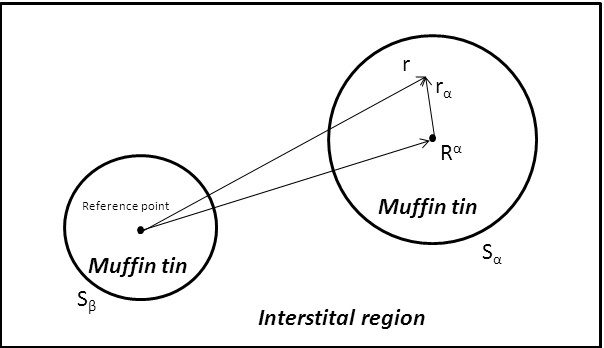
\includegraphics[scale=0.7]{Presentation1.png}
\caption{Partition of the unit cell.}
\label{ucuc}
\end{center}
\end{figure}

From the \textbf{Fig. \ref{ucuc}}, one will notice that the unit cell is divided into muffin-tin spheres ($\alpha$, $\beta$) and an
interstitial region (IR), and ${\textbf r={\textbf R^{\alpha}}+{\textbf r_{\alpha}}}$ is guaranteed. One can take use of the Rayleigh expansion formula:

\begin{equation}
\expg<(\textbf {k+G})>= e^{i (\textbf {k+G}) \textbf{R}^{\alpha} } 4 \pi \sumlm<\ell><m> i^{\ell} \bessf< |\textbf{k+G}|> \sphfr<\ell{m}><r><> \sphfq<\ell{m}><\textbf{k+G}><*> .
\end{equation}
  
After matching those two representation, the following equation is satisfied for each ${\ell}m$:

\begin{equation}
A _{{\ell}m}^{\alpha} (\textbf {k+G})= \frac{ e^{i (\textbf {k+G}) \textbf{R}^{\alpha} } 4 \pi \sumlm<\ell><m> i^{\ell} \bessf< |\textbf{k+G}|> \sphfq<\ell{m}><\textbf{k+G}><*> }{\sqrt{\Omega} u_{{\ell}}^{\alpha}(r_{\alpha}, E)}.
\end{equation}

There are one main drawbacks about the APW method. The wavefuntion is energy dependent, which means that
 the code will search for the energy in order to calculate the exact energy. Therefore it 
is really time consuming. 

\subsubsection{Linearized augmented plane wave method}
\noindent In order to decouple the energy and wavefunction, Andesen, Koelling and Arbman found out a way to seperate them, they noticed that the taylor expansion of the radial function
on certain energy, which can be expressed as follows:

\begin{equation}\label{ap3}
 u_{{\ell}}^{\alpha}(r_{\alpha}, E) = u_{{\ell}}^{\alpha}(r_{\alpha}, E_{\ell}) + (E-E_{\ell}) \dot{u}_{{\ell}}^{\alpha}(r_{\alpha}, E_{\ell}) + O((E-E_{\ell})^2).
\end{equation}

Therefore they re-defined the wavefuntion in the following way:

\begin{equation}\label{lap4}
\phi^{LAPW}_\textbf{k+G} (\textbf{r})= 
\begin{cases} \frac {1}{\sqrt{\Omega}} e^{i(\textbf{k+G})\textbf{r}} & \quad \mbox{if $\textbf{r} \in I $}
\\
\sumg<\alpha>\sum\limits_{{\ell}m} f_{{\ell}{m}} (r_{\alpha},\textbf{k+G}, E_{\ell}) Y_{{\ell}m}(\hat{\textbf{r}}_{\alpha})  & \quad \mbox{if $\textbf{r} \in S_\alpha, $}\\ 
\end{cases}
\end{equation}

where $f_{{\ell}{m}} (r_{\alpha},\textbf{k+G} ,E_{\ell}) =  A _{{\ell}m}^{\alpha} (\textbf {k+G}) u_{{\ell}}^{\alpha}(r_{\alpha}, E_{\ell}) + B _{{\ell}m}^{\alpha} (\textbf {k+G}) \dot{u}_{{\ell}}^{\alpha}(r_{\alpha}, E_{\ell})$
. $A _{{\ell}m}^{\alpha} (\textbf {k+G})$ and $B _{{\ell}m}^{\alpha} (\textbf {k+G})$ are the expansion coefficients, and $\dot{u}_{{\ell}}^{\alpha}(r_{\alpha}, E_{\ell} )$ is the derivative of the radial function.

Here energy $E_{\ell}$  is considered as pre-calculated parameter, actually, it is chosen by the middle of  each $\ell$-character band, therefore this method is called linearized augmented plane wave (LAPW) method.

Apparently, LAPW method is more suitable in reality, because the wavefunction is decoupled with energy, but it has to match for two parameters,
fortunately, even though, it still use less time comparing with APW method. However, there is one drawback about this method, what if energy difference is bigger enough in the same $ {\ell} $ charater, 
which $E_{\ell}$ is correct one? Therefore this situation could be a big error, these states are called as semi-core state, for example, it exists in the actinides and the rare earths.

\subsubsection{Linearized augmented plane wave method plus local orbitals}
Comparing with LAPW method, Linearized augmented plane wave method plus local orbitals (LAPW+LO) method extend the basis set, and add smaller number of basis set, which has the following format:


\begin{equation}\label{lap5}
\phi^{LO}_\textbf{k+G} (\textbf{r})= 
\begin{cases} 0 & \quad \mbox{if $\textbf{r} \in I $}
\\
(A _{{\ell}m}^{\alpha}  u_{{\ell}}^{\alpha}(r_{\alpha}, E_{\ell}) + B _{{\ell}m}^{\alpha}  \dot{u}_{{\ell}}^{\alpha}(r_{\alpha}, E_{\ell}) + C _{{\ell}m}^{\alpha}  u_{{\ell}}^{\alpha}(r_{\alpha}, E^{\prime}_{\ell})){Y_{{\ell}m}(\hat{\textbf{r}}_{\alpha})} & \quad \mbox{if $\textbf{r} \in S_\alpha, $}\\ 
\end{cases}
\end{equation}
 
where $A _{{\ell}m}^{\alpha}$ and $B _{{\ell}m}^{\alpha}$ is matching value and derivate on the sphere boundary to zero, but not plane wave, and $E^{\prime}_{\ell}$ is
the chosen energy from semi-core state.

\subsubsection{Augmented plane wave method plus local orbitals}

Actually, there is one more method which will deal with the energy-denpendent case, which is called as augmented plane wave method plus local orbitals (APW+lo), the 
basis function has two kinds, one is similar with APW method, but only without the derivative terms, e.g., $f_{{\ell}{m}} (r_{\alpha},\textbf{k+G} ,E_{\ell}) =  A _{{\ell}m}^{\alpha} \textbf(k+G) u_{{\ell}}^{\alpha}(r_{\alpha}, E_{\ell})$.
Another basis function is:
\begin{equation}\label{lap6}
\phi^{lo}_\textbf{k+G} (\textbf{r})= 
\begin{cases} 0 & \quad \mbox{if $\textbf{r} \in I $}
\\
(A _{{\ell}m,lo}^{\alpha}  u_{{\ell}}^{\alpha}(r_{\alpha}, E_{\ell}) + B _{{\ell}m,lo}^{\alpha}  \dot{u}_{{\ell}}^{\alpha}(r_{\alpha}, E_{\ell}) ){Y_{{\ell}m}(\hat{\textbf{r}}_{\alpha})} & \quad \mbox{if $\textbf{r} \in S_\alpha. $}\\ 
\end{cases}
\end{equation}
 
The value of $A _{{\ell}m,lo}^{\alpha}$ and $B _{{\ell}m,lo}^{\alpha}$ are obtained by normalization and local orbital has zero value at the muffin tin boundary. This method can not deal with semicore states like LAPW+LO, 
however, it does increase the efficiency to linearize Slater's APW method.

\subsection{Effective potential}

\label{epote}
The potential in the FP-LAPW method is also divided into two regions, the MT region and the interstitial region.
\begin{equation*}\label{lap7}
V(\textbf{r})= 
\begin{cases} \sumg<{\textbf G}> V_{\textbf G} e^{i {\textbf G} {\textbf {r}  }} & \quad \mbox{if $\textbf{r} \in I $}
\\
 \sum\limits_{{\ell}m} V_{{\ell}m}^{\alpha} (r_{\alpha}) Y_{{\ell}m}(\hat{{\textbf r}}_{\alpha})  & \quad \mbox{if $\textbf{r} \in S_\alpha. $}\\ 
\end{cases}
\end{equation*}

\section{Dielectric function}
The dielectric function describes the optical property of materials. Normally, it is written as $\varepsilon$, which has two parts:

\begin{equation}
 \varepsilon = \varepsilon_1 + i \varepsilon_2,
\end{equation}

where $\varepsilon_1$ denotes how much the material is polarized when an electric field is applied, and $\varepsilon_2$ is related with absorption of the material.

Here a summary of the basic derivation of dielectric function is presented using random-phase approximation (RPA).

Response to external electric field $E$ in the linear approximation:
\begin{equation}\label{df1}
D = \varepsilon E,
\end{equation}
where $D$ is electric displacement, and $E$ is the electric field.

After some derivations, the imaginary part of $\varepsilon$ is:
\begin{equation}\label{df2}
\varepsilon_2 = \frac{4 \pi e^2}{m^2\omega^2} \sum_{cv} \int d \textbf {k} <\Psi_{c{\textbf k}}|p^\alpha|\Psi_{v{\textbf k}}><\Psi_{v{\textbf k}}|p^\beta|\Psi_{c{\textbf k}}>\delta(\varepsilon_{c {\textbf k}}-\varepsilon_{c{\textbf k}}-\omega),
\end{equation}
where $c$ and $v$ run over the conduction bands and valence bands, for example, one can find the figure which is calculated using this equation in the paper of $??$.

The interband contribution of dielectric function is:
\begin{equation}\label{df2}
\varepsilon_2 = \frac{4 \pi e^2}{m^2\omega^2} \sum_{cv} \int d \textbf {k} <\Psi_{c{\textbf k}}|p^\alpha|\Psi_{v{\textbf k}}><\Psi_{v{\textbf k}}|p^\beta|\Psi_{c{\textbf k}}> (f(\varepsilon_{c \textbf k})-f(\varepsilon_{v \textbf k}))\delta(\varepsilon_{c {\textbf k}}-\varepsilon_{c{\textbf k}}-\omega),
\end{equation}
which is often calculated in the field that is related to optical property, for example, it is calculated in the paper of $??$, which is plotted in the Fig.$??$ of
that paper.

Here only some very basic equations are covered when it is related to calculate the dielectric function. If someone is interested in this topic, one can find more detailed in Ref. $??$.

\begin{comment}
\section{k $\cdot$ p method}
\label{kpmaa}

The band dispersion can be obtained exactly by using the $\bold k \cdot \bold p$ method in principle, the basic idea will be explained in the following text.

First, if the Schrödinger equation is defined as follows:

\begin{equation}\label{kpse}
\left\{ \frac {{\textbf p}^2} {2m} + V({\textbf r}) \right\} \wfbloch<n>< \bold k> = \ebloch<n><\bold k> \wfbloch<n><\bold k>,
\end{equation}

where ${\textbf p} = i \hbar \bigtriangledown $, and the Bloch theory shows:

\begin{equation}\label{1}
 \wfbloch<n><\bold k> = \expg<k> \ubloch<n><\bold k>,
\end{equation}

where $\wfbloch<n><\bold k>$ is the wavefunction on ${\textbf k}$ point for the {$\textit n$}th band, and $\expg<k>$ is plane wave, $\ubloch<n><\bold k>$ is a function which has the same a periodicity as the potential.

If substituting the Eq. \ref{1} to Eq. \ref{kpse}, it will end up the following equation:

\begin{equation}
 \{  \frac{{\textbf p}^2}{2m} + V({\textbf r }) + \frac{{\hbar^2 {\textbf k}^2}}{2m} + \frac{{\hbar \textbf {kp}}}{m} \} \ubloch<n><\bold  k>  =  \ebloch<n><\bold  k> \ubloch<n><\bold  k>.
\end{equation}

In the above equation, if $\textbf k = \textbf 0$, then the Hamiltonian turn out to be $H_0 = {\textbf p}^2 / {2m} + V({\textbf r })$. Here the first two terms are treated as unpertubation term, and pertubation term is seen as
$W={{\hbar^2 {\textbf k}^2}}/{2m} + {{\hbar \textbf {kp}}}/{m}$, the result will be as follows after treating the equation as pertubation.

\begin{equation}
 \ebloch<n><\bold k> = E_{n,\textbf 0} + \frac{{\hbar^2 {\textbf k}^2}}{2m} + \frac{ \hbar^2}{m^2} \suminj<i><j> \frac{|<\ubloch<n><\bold 0>|{\textbf {kp}}|\ubloch<n'><\bold  0>>|^2}{E_{n,\textbf 0} - E_{n',\textbf 0}}.
\end{equation}


Now let us suppose the wavefunction and energy are obtained by some procedures on $\bold k_0$ point, $\wfbloch<n><\bold  k_0>$ is the wavefunction and $\ebloch<n><\textbf  k_0>$ is the energy.
Another function is defined as follows:

\begin{equation}\label{2}
\chikp<n><\textbf k> = \expg<(\bold k-\bold {k_0})>  \wfbloch<n><\bold {k_0}>.
\end{equation}

The above function $\chikp<n><\textbf k> $ is expanded as wavefunction on ${ \textbf k}$ point, and then the wavefunction on the ${\textbf k}$ point is calculated by:
\begin{equation}\label{3}
\wfbloch<n><\bold k> =  {\sum\limits_{j}} C_{n,j}^{\bold k} \chikp<j><\bold k>. 
\end{equation}

From above equation, the wavefunction is known if the coefficient $C_{n,j}^{\bold k}$ is obtained, let us substitute the Eq. \ref{3} into Kohn-Sham Eq. \ref{kpse}.
Finally the following equation is obtained:

\begin{equation}\label{5}
{\sum\limits_{j}}  C_{n,j}^{\bold k} \left \{  \left [  \ebloch<j><\bold {k_0}> -  \ebloch<n><\bold k>  + \frac{{\hbar}^2}{2m} { (\bold {k}^2- \bold {k}_0^2)}    \right ] \delta_{j',j} + \frac{\hbar}{m} {(\bold {k}-\bold{k}_0)} {\overline{\textbf{p}}_{j',j}} \right \} = 0,
\end{equation}

where ${\overline{\textbf{p}}_{j',j}} = \langle \ubloch<j'><\bold {k_0}>| {\textbf p} | \ubloch<j><\bold {k_0}>  \rangle $.
 
We also can simpify the above equation in the following format:
\begin{equation}\label{6}
{\sum\limits_{j}} C_{n,j}^{\bold {k}} \left \{ H_{j',j}- \ebloch<n><\bold {k}> \delta_{j',j} \right \} =0,
\end{equation}

where
\begin{equation} \label{7}
H_{j',j} = \left [  \ebloch<j><\bold {k_0}>  + \frac{{\hbar}^2}{2m} { (\bold{k}^2-\bold{k}_0^2)}    \right ] \delta_{j',j} + \frac{\hbar}{m} {(\bold{k}-\bold{k}_0)} {\overline{\textbf{p}}_{j',j}}.
\end{equation}

From the above equation, the coefficient $ C_{n,j}^{\bold k}$ and $\ebloch<n><\bold {k}>$ are calculated.

\section{Scalar relativistic approximation and spin-orbit coupling}
\label{srasoc}

\subsection{Dirac equation}

Non-relativistic quantum mechanics has broad application, but when the speed of electron is near the speed of light, 
the non-relativistic quantum is not suitable to describe the system of electron. So Dirac introduced an equation which is called
Dirac equation applying for relativistic case.

\noindent Dirac defined the Hamiltonian: 

\begin{equation}\label{dirac}
\hat{H}_\textit{dirac} = c \boldsymbol{\alpha} \textbf{P} + \boldsymbol{\beta}mc^{2} + V
\end{equation}

\noindent where $\textbf{P} = -i\hbar \nabla $ is the momentum operator,$V$ is the general potential, $m$ is the mass of electron 
and $c$ is the speed of light, $\boldsymbol{\alpha}$ and $\boldsymbol{\beta}$ are $4 \times 4$ matrices.
\begin{equation}
 \boldsymbol{\alpha} = \left( \begin{array}{cc}
 0 & \boldsymbol{\sigma}  \\
 \boldsymbol{\sigma} & 0   \end{array} \right),
\boldsymbol{\beta}= \left( \begin{array}{ccc}
\boldsymbol{I} & 0\\
0 & -\boldsymbol{I}\end{array} \right)
\end{equation}

\noindent where $\boldsymbol{I}$ is unit matrix, and $\boldsymbol{\sigma}$ is Pauli matrix.

\begin{equation} 
\boldsymbol{\sigma} = (\boldsymbol{\sigma}_x \  \boldsymbol{\sigma}_y \  \boldsymbol{\sigma}_z )  
\end{equation}

\begin{equation}
\boldsymbol{\sigma}_x= \left( \begin{array}{cc}
0 & 1\\
1 & 0\end{array} \right),
\boldsymbol{\sigma}_y= \left( \begin{array}{ccc}
0 & -i\\
i & 0\end{array} \right),
\boldsymbol{\sigma}_z= \left( \begin{array}{ccc}
1 & 0\\
0 & -1\end{array} \right)
\end{equation}

\subsection{Derivation of ????}

\noindent  $\Psi$ is the wavefunction of Hamiltonian \ref{dirac}, which has four components, but can be 
written with only two terms:
\begin{equation}\label{diracwf}
\Psi= \left( \begin{array}{c}
\phi^{\uparrow} \\
\phi^{\downarrow} \\
\chi^{\uparrow} \\
\chi^{\downarrow} \end{array} \right),
 \Psi = \left(\begin{array}{c}
\phi \\               
\chi \end{array} \right)
\end{equation}

\noindent where $\phi$ includes the two terms of $\phi^{\uparrow}$ and $\phi^{\downarrow}$, and $\chi$ contains  $\chi^{\uparrow}$ and $\chi^{\downarrow}$;
under the nonrelativistic limit,$\phi$ is bigger than $\chi$ by the ratio of $v/c$, where $v$ and $c$ are speed of particle and light, respectively,
so the $\phi$ is the large term and $\chi$ is the small one.

\noindent In order to derive the scalar relativistic approximation and the spin-orbit coupling terms, we need to take use of the nonrelativistic limit approximation of the 
Dirac eigenvalue equation probelm, here nonrelativistic limit means $v^2/c^2 << 1$.

\begin{equation}\label{diracse}
 E \Psi = (c \boldsymbol{\alpha} \textbf{P} + \boldsymbol{\beta}mc^{2} + V) \Psi
\end{equation}

\noindent For convenience, we define:

\begin{equation}\label{dirace}
E^{\prime} = E - mc^2
\end{equation}

\noindent where $E$ is the total energy, $mc^2$ are $E'$ are the rest mass energy and the remaining energy excluding the rest mass energy, under the nonrelativistic limit, 
$E'$ is far smaller than $mc^2$. Now, putting equation \ref{diracwf} and \ref{dirace} into equation \ref{diracse}:

\begin{equation}
\begin{split}
&(E^{\prime} - V) \Phi - c \boldsymbol{\sigma} \textbf{P} \chi = 0\\                
&-c\boldsymbol{\sigma} \textbf{P} \Phi + (E^{\prime}+2mc^2-V)\chi = 0
\end{split}
\end{equation}

\noindent To eliminate the $\chi$ (otherwise, it is the antiparticle problem), we can end up with the equation:
  \begin{equation}
(V + \frac{1}{2m} (\boldsymbol{\sigma} \textbf{P}) (1+\frac{E^{\prime}-V}{2mc^2})^{-1} (\boldsymbol{\sigma} \textbf{P}) )\phi=E^{\prime}\phi
\end{equation}

\noindent Since ${E^{\prime}-V}$ is far smaller than ${2mc^2}$, so taking advantage of the taylor expansion and the following identites:
\begin{equation}
\begin{split}
& [\textbf{P}, V ]= -i \hbar \triangledown V \\                
&(\boldsymbol{\sigma} \textbf{A} )(\boldsymbol{\sigma} \textbf{B}) = \textbf{A} \textbf{B} + i\boldsymbol{\sigma}[\textbf{A} \times \textbf{B}]
\end{split}
\end{equation}

After some operations, we finally will get the following equation under the nonrelativistic limit:

\begin{equation}
E^{\prime} \phi = (\frac{\textbf{P}^2}{2m} + V - \frac{\textbf{P}^4}{8 {m}^3 {c}^2}-\frac{i\hbar}{4{m}^2 {c}^2} (\nabla{V})\textbf{P}+\frac{\hbar}{4 m^2 c^2} \boldsymbol{\sigma}[\nabla{V} \times \textbf{P}]) \phi
\end{equation}

Furthermore, we can approximate the above equation to the simpler expression under spherical symmetry potential:

\begin{equation}
 E^{\prime} \phi = (\frac{\textbf{P}^2}{2m} +V - \frac{\textbf{P}^4}{8 {m}^3 {c}^2}-\frac{i\hbar}{4{m}^2 {c}^2} (\nabla{V})\textbf{P}+\frac{1}{2 m^2 c^2} \frac{1}{R} \frac{dV}{dR}\textbf{S}\textbf{L}) \phi
\end{equation}

\noindent where $\textbf{S}={\hbar}{\boldsymbol{\sigma}}/2$ is the Pauli spinor, and $\textbf{L}=\textbf{R} \times \textbf{P}$ is the orbital
angular momentum operator. The terms of ${\textbf{P}^2}/(2m) + V$ is Schrödinger term,  ${\textbf{P}^4}/(8 {m}^3 {c}^2)$ and ${i\hbar} (\nabla{V})\textbf{P} /(4{m}^2 {c}^2)$  are the mass enhancement 
and Darwin term, respectively, both of them together is called the scalar relativistic approximation (SRA), the last term is the spin-orbit coupling (SOC) term. One has to
notice that the Darwin term is not hermitian operator, alternatively, which will be $\nabla^2{V} /(8{m}^2 {c}^2)$ instead in the realistic implementation.

\end{comment}

\chapter{Results and discussion}

In this chapter, the major result for the doctoral training is demonstrated. It has two branches, one is the result from the point of modeling and calculations for the thin film materials copper indium gallium (di)selenide (CIGS)
 and copper zinc tin sulfide/selenide (CZTS/Se), the other is methodology, which includes the result from scalar relativistic approximation (SRA) and spin-orbit coupling (SOC).

\section{Modeling and calculations}

\subsection{Copper indium gallium diselenide}
In this section, the parameterization of $\cigs$ (x=0, 0.5, and 1) energy bands is described firstly. Afterwards some results based on this parameterization are demonstrated. At last, calculation of the 
dielectric function spectra for the material $\mathrm{CuIn_{0.5}Ga_{0.5}Se_2}$ is presented and analyzed. Moreover, it compared with experimental results as well.

\subsubsection{Parameterization of energy bands}
The curvature of energy bands is often demonstrated by the effective electron and hole masses, therefore the parabolic energy dispersion of energy bands, also named parabolic band approximation (pba), is 
assumed normally:

\begin{equation}\label{parabolic}
E_{j}^{pb}(\textbf{k}) = E_{j}(\textbf{0}) \pm \left[ \frac{\widetilde{\textbf{k}}_{x}^{2}+\widetilde{ \textbf{k}}_{y}^{2}}{m_{j}^{\perp}} + \frac{\widetilde{\textbf{k}}_{z}^{2}}{m_{j}^{\parallel}} \right],
\end{equation}

where $m_{j}^{\perp}$ is transverse electron masses and $m_{j}^{\parallel}$ is longitudinal electron masses.
 
Unfortunately, these effective masses are only valid around the considered {\textbf k} point, which is not suitable to describe the non-parabolic away from this {\textbf k} point.
However, the accurate shape of energy bands is important when one simulates and analyzes the electron transport or band filling for some materials.

In this work, we have parameterized the three uppermost valences bands (VBs) and the lowest conduction band (CB) for the materials $\cigs$ where $x$=0, 0.5, and 1, that is,
$\mathrm{CuInSe_2}$, $\mathrm{CuIn_{0.5}Ga_{0.5}Se_2}$, and $\mathrm{CuGaSe_2}$. This parameterization is based on the all electron and full-potential linearized augemented plane wave (FP-LAPW) calculation.
Normally, the \textbf{k $\cdot$ p} method is utilized to parameterize the energy bands. However, due to the crystal-field interaction and the spin-orbit coupling, 
the energy dispersions of $\cigs$ are rather complex, therefore, the regular \textbf{k $\cdot$ p} method is not sufficient to describe the energy bands. 
We manage to extend the \textbf{k $\cdot$ p} expression to higher orders, which is called full band parameterization (fbp) in the following text. Finally, the following equation is used to parameterize the energy bands,
 which is valid around 0.5 eV below VBM and 0.5 eV above CBM.

\begin{equation}\label{nonparabolic}
\begin{split}
& \small E_j(\textbf{k}) = E_{j}^{pb}(\textbf{k}) + E_j^0 + \Delta_{j,1} \left( \delta_{j,1}^2 \left( \frac{\widetilde{\textbf{k}}_{x}^{4}+\widetilde{ \textbf{k}}_{y}^{4}}{m_{0}^{2}} \right) + \delta_{j,2}^2 \left( \frac{\widetilde{\textbf{k}}_{x}^{2}\widetilde{\textbf{k}}_{y}^{2}}{m_{0}^2} \right) + 1 \right)^{1/2} \\
& \small + \Delta_{j,2} \left( \delta_{j,3}^3 \left( \frac{\widetilde{\textbf{k}}_{x}^{6}+\widetilde{ \textbf{k}}_{y}^{6}}{m_{0}^{3}} \right) + \delta_{j,4}^3 \left( \frac{\widetilde{\textbf{k}}_{x}^{2}\widetilde{\textbf{k}}_{y}^{4} + \widetilde{\textbf{k}}_{x}^{4}\widetilde{\textbf{k}}_{y}^{2}}{m_{0}^3} \right) + 1 \right)^{1/3} \\
& \small + \Delta_{j,3} \left( \delta_{j,5}^2 \left( \frac{\widetilde{\textbf{k}}_{z}^{4}}{m_0^2} \right) + 1 \right)^{1/2} + \Delta_{j,4} \left( \delta_{j,6}^3 \left( \frac{\widetilde{\textbf{k}}_{z}^{6}}{m_0^3} \right) + 1 \right)^{1/3} \\
& \small + \Delta_{j,5} \left( \delta_{j,7}^2 \left( \frac{\widetilde{\textbf{k}}_{x}^{2}\widetilde{\textbf{k}}_{z}^{2} + \widetilde{\textbf{k}}_{y}^{2}\widetilde{\textbf{k}}_{z}^{2}}{m_{0}^3} \right) + 1 \right)^{1/2} \\
& \small + \Delta_{j,6} \left( \delta_{j,8}^3 \left( \frac{\widetilde{\textbf{k}}_{x}^{4}\widetilde{\textbf{k}}_{z}^{2} + \widetilde{\textbf{k}}_{y}^{4}\widetilde{\textbf{k}}_{z}^{2}}{m_{0}^3} \right) + \delta_{j,9}^3 \left( \frac{\widetilde{\textbf{k}}_{x}^{2}\widetilde{\textbf{k}}_{z}^{4} + \widetilde{\textbf{k}}_{y}^{2}\widetilde{\textbf{k}}_{z}^{4}}{m_{0}^3} \right) + \delta_{j,10}^3 \left( \frac{\widetilde{\textbf{k}}_{x}^{2}\widetilde{\textbf{k}}_{y}^{2}\widetilde{\textbf{k}}_{z}^{2}}{m_{0}^3} \right) +1 \right)^{1/3},
\end{split}\end{equation}

where  $E_j^0$, $\Delta_{j,n}$, and $\delta_{j,m}$ are fitting parameters, ${m_0}$ is the electron rest mass. In the Eq. \ref{nonparabolic}, each term represents one
parabolic dispersion, the higher order terms describe the larger wave vectors away from $\Gamma$ point. Unfortunately, the complex
energy dispersions of $\cigs$ requires many fitting parameters. However, the conduction band need less fitting parameters.

 \newpage

\begin{table}[ht]
\caption{Parameters of equation \ref{parabolic}}
\begin{center}
\begin{tabular}{ccc}
\end{tabular}
\end{center}
\label{rd1}
\end{table}

\begin{table}[ht]
\caption{Parameters of equation \ref{nonparabolic}}
\begin{center}
\begin{tabular}{ccc}
\end{tabular}
\end{center}
\label{rd2}
\end{table}


 \newpage

Firstly, the fbp of $\cigs$ ($x$= 0, 0.5, and 1) are plotted compared with the calculation based on the FP-LAPW method and the pba in 
Eq. \ref{parabolic}.

\begin{figure}[H]
    \begin{center}
            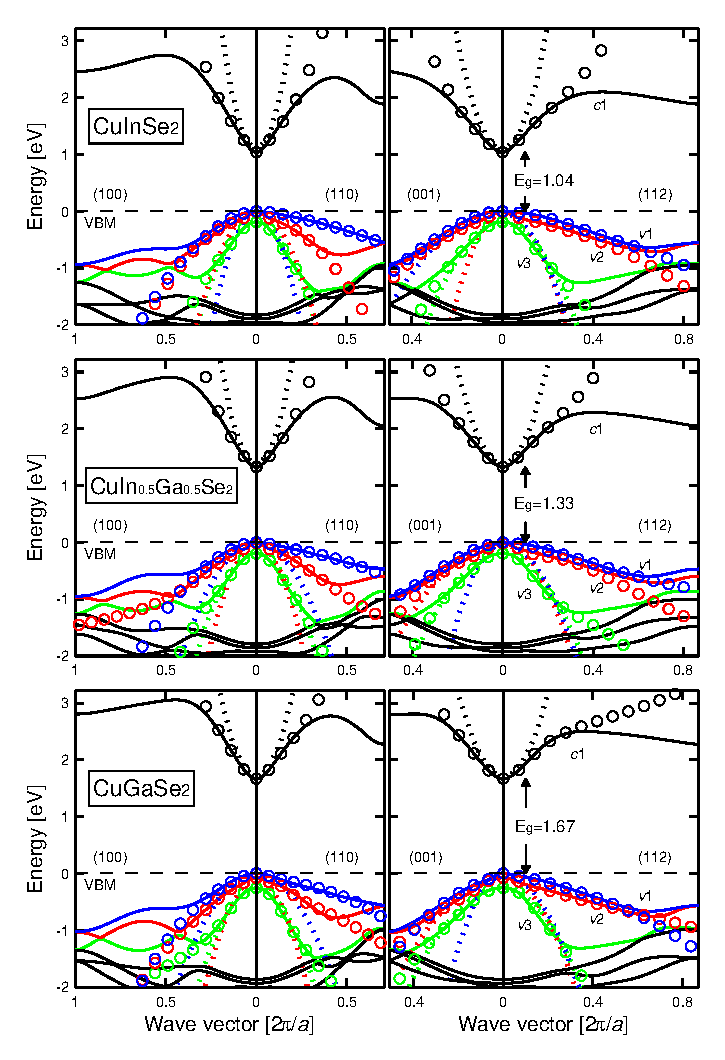
\includegraphics[width=0.45\textwidth,clip]{paper2figure1}
            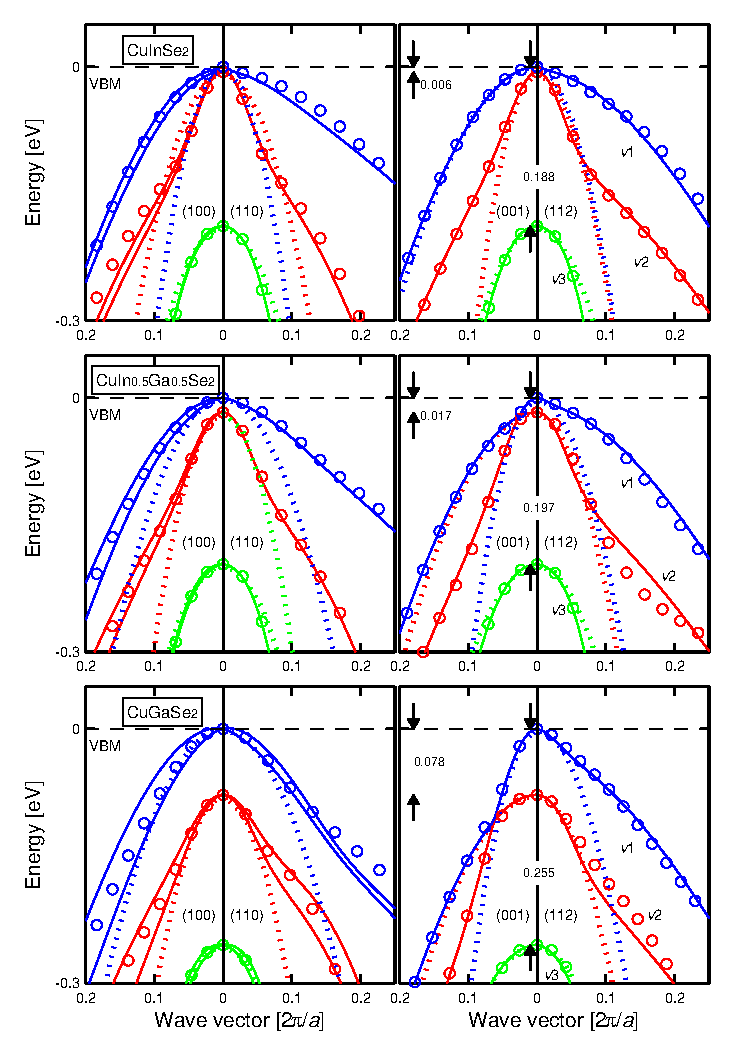
\includegraphics[width=0.46\textwidth,clip]{paper2figure2}
     \end{center}
    \caption{ Left panel: Electronic band structure along four directions.
 the circles are the results of the full band parameterization (fbp), 
and the dotted lines represent the parabolic band approximation (pba). 
Righ panel: The close-up of left panel for the valence bands close to $\Gamma$ point.}      
    \label{bandstruct}
\end{figure}

From \textbf{Fig. \ref{bandstruct}}, one will observe that the parameterized energy bands can describe the energy below VBM around 0.5 eV accurately, and around 0.5 eV above the CB minimum (CBM) as well.
However, the pba is only valid below VBM around -4, -10, and -40 meV for $\mathrm{CuInSe_2}$, $\mathrm{CuIn_{0.5}Ga_{0.5}Se_2}$, and $\mathrm{CuGaSe_2}$,
respectively. Since the lowest conduction band is more parabolic, therefore, the less fitting parameters are expected (Table \ref{rd2}).

In order to demonstrate the anisotropic and non-parabolic of energy bands, some properties are investigated, such as effective 
electron and hole masses and constant energy surface.

\begin{figure}[H]
    \begin{center}
            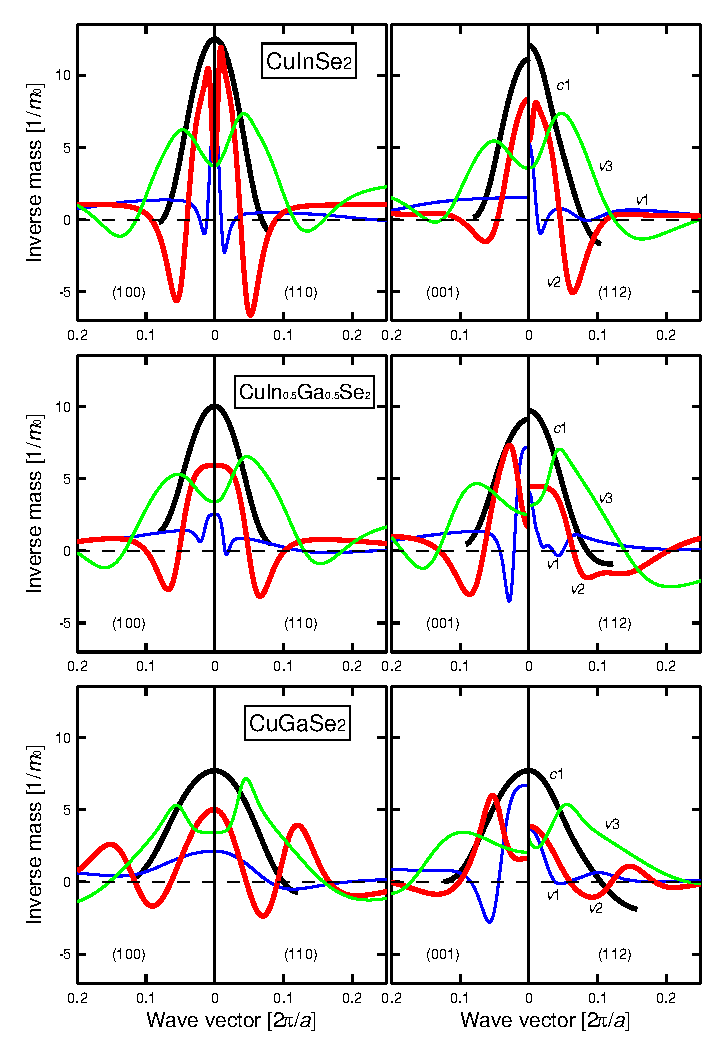
\includegraphics[width=0.45\textwidth,clip]{paper1figure3}
     \end{center}
    \caption{ Inverse of the effective electron and hole masses in the four symmetry directions for the $\cigs$ (x=0, 0.5, and 1).}      
    \label{inversemessf}
\end{figure}

The effective masses are calculated numerically by:

\begin{equation}\label{inversemasse}
m_j(\textbf{k}) = \pm \hbar^2/(\partial^2 E_j(\textbf{k})/\partial\textbf{k}^2).
\end{equation}
 
In order to better visibility, therefore, the inverse of the mass are presented. The result from \textbf{Fig. \ref{inversemessf}} demonstrates that the energy bands of $\cigs$
are strong non-parabolic, since it should be constant in the pba along each symmetry direction. The effective hole masses of the two topmost VBs are very anisotropy close
to the $\Gamma$ point, however, the electron masses of conduction bands are rather isotropic ($m_{c1}^{100}(\textbf{0}) \approx m_{c1}^{110}(\textbf{0}) \approx m_{c1}^{001}(\textbf{0}) \approx m_{c1}^{112}(\textbf{0})$).

To further demonstrate the non-parabolic of energy bands, the constant energy surfaces for $CuInSe_2$ and $CuGaSe_2$ are plotted.

\begin{figure}[H]
    \begin{center}
            \includegraphics[width=0.46\textwidth,clip]{fermi_sphere_cii}
           % \includegraphics[width=0.4\textwidth,clip]{fermi_sphere_cig}
            \includegraphics[width=0.4\textwidth,clip]{fermi_sphere_cgg}
     \end{center}
    \caption{Constant energy surfaces for the three uppermost VBs and the lowest CB for the energies E = 1 meV (left column ellipsoidal) and E = 200 meV (right column).  
The $CuInSe_2$ and $CuGaSe_2$ are demonstrated in this figure.}
    \label{cse}
\end{figure}

In the \textbf{Fig. \ref{cse}}, 1 meV represents that it is near to $\Gamma$ point ; 200 meV means that it is far away the $\Gamma$ point.
One will notice that the pba is proper to describe the energy bands close to the $\Gamma$ point, and it is ellipsoidal shaped sphere. For example,
for the topest VB ($v_1$) of $\mathrm{CuInSe_2}$, the constant energy surface is ellipsoidal in the vicinity of the $\Gamma$ point since the effective
masses are anisotropic ($m_{v1}^{\perp}$=0.14$m_0$ and $m_{v1}^{\parallel}$=0.66$m_0$). However, the constant energy surface becomes non-ellipsoidal when the energies 
is far away from $\Gamma$ point. For example, for the same band, the constant energy surface is not ellipoidal shape at all when the energies goes up to 200 meV.

In order to analyze the impact of non-parabolicity and anisotropy of the energy bands, some properties are compared in the following text between fbp and pba, respectively, such as density-of-states (DOS),
DOS mass, carrier concentration in intrinsic and p-type of $\cigs$.

The DOS in $j$th band is defined as:

\begin{equation}\label{dosj}
 g_j(E)=\frac{1}{\Omega} \sum \limits_{\textbf{k}} 2 \delta (E-E_j(\textbf{k})) = \frac{1}{4\pi^3} \int \limits_{E_j(\textbf{k}) = E} \frac{dS(\textbf{k})}{|\bigtriangledown_\textbf{k} E_j(\textbf{k})|},
\end{equation}
 
where $E_j(\textbf{k}) = E$ is the $\textbf{k}$ space surface with constant energy $E$, and the $\bigtriangledown_\textbf{k} E_j(\textbf{k})$ is the gradient of the energy dispersion.
In the case of the pba, the Eq. \ref{dosj} will be written:

\begin{equation}\label{dosjp}
 g_j^{pba}(E) = \frac{1}{2\pi^2} \big(\frac{2m_j^{DOS}}{\hbar^2}\big)^{3/2} \sqrt{|E-E_j(\textbf{0})|},
\end{equation}
 
where the DOS mass $m_j^{DOS}$ is equal to $\big( m_j^{\perp}m_j^{\perp}m_j^{\parallel} \big)^{1/3}$, which reprents the extent of filling the specific band with free carriers to certain energy. 
In order to take advantage of the simple Eq. \ref{dosjp} for the non-parabolic energy bands, the energy-dependent DOS mass ($m_{v/c}^{DOS}$) is defined:

\begin{equation}\label{dosmass}
 g_{v/c}(E) = \sum \limits_j g_j(E) = \frac{1}{2\pi^2} \big(\frac{2m_{v/c}^{DOS}(E)}{\hbar^2}\big)^{3/2} \sqrt{|E-E_{v1/c1}(\textbf{0})|}.
\end{equation}

where the DOS mass contains the non-parabolicity and anisotropy of the band dispersion.

 \begin{figure}[H]
  \begin{center}
            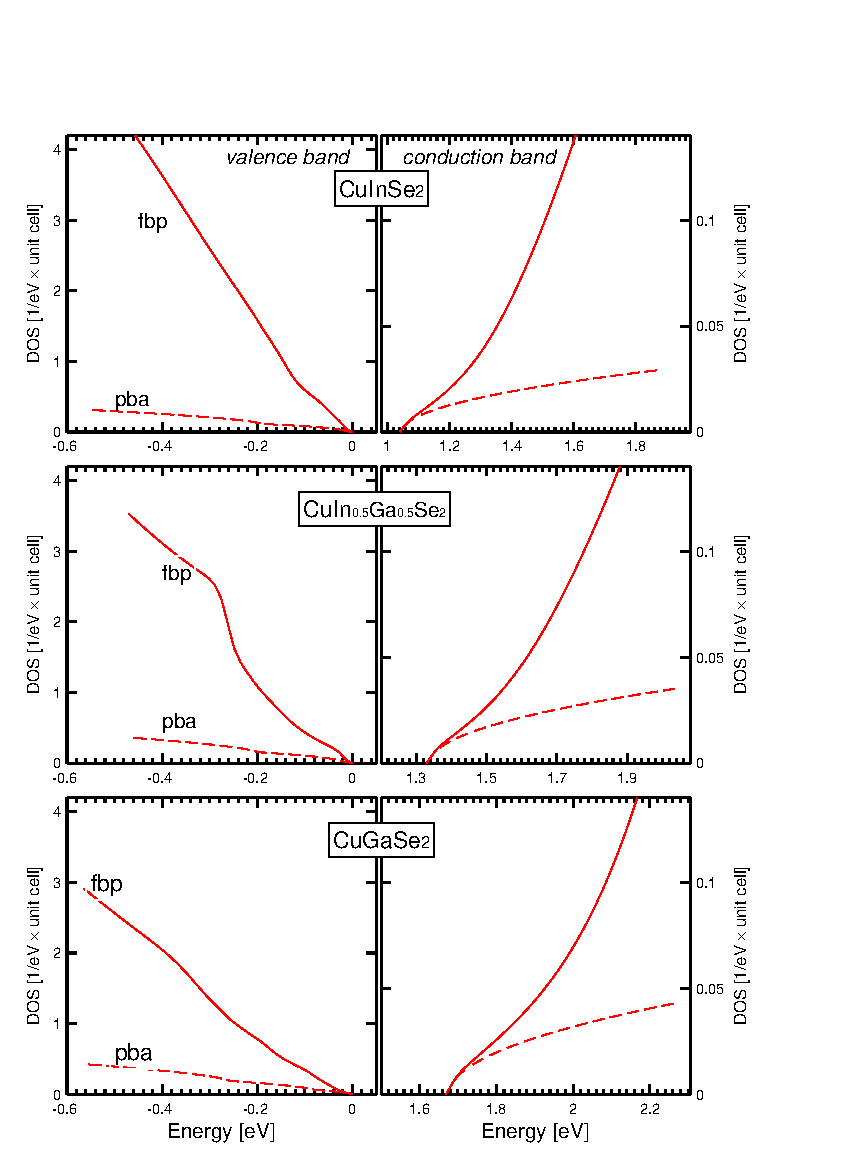
\includegraphics[width=0.48\textwidth,clip]{paper2figure4}
            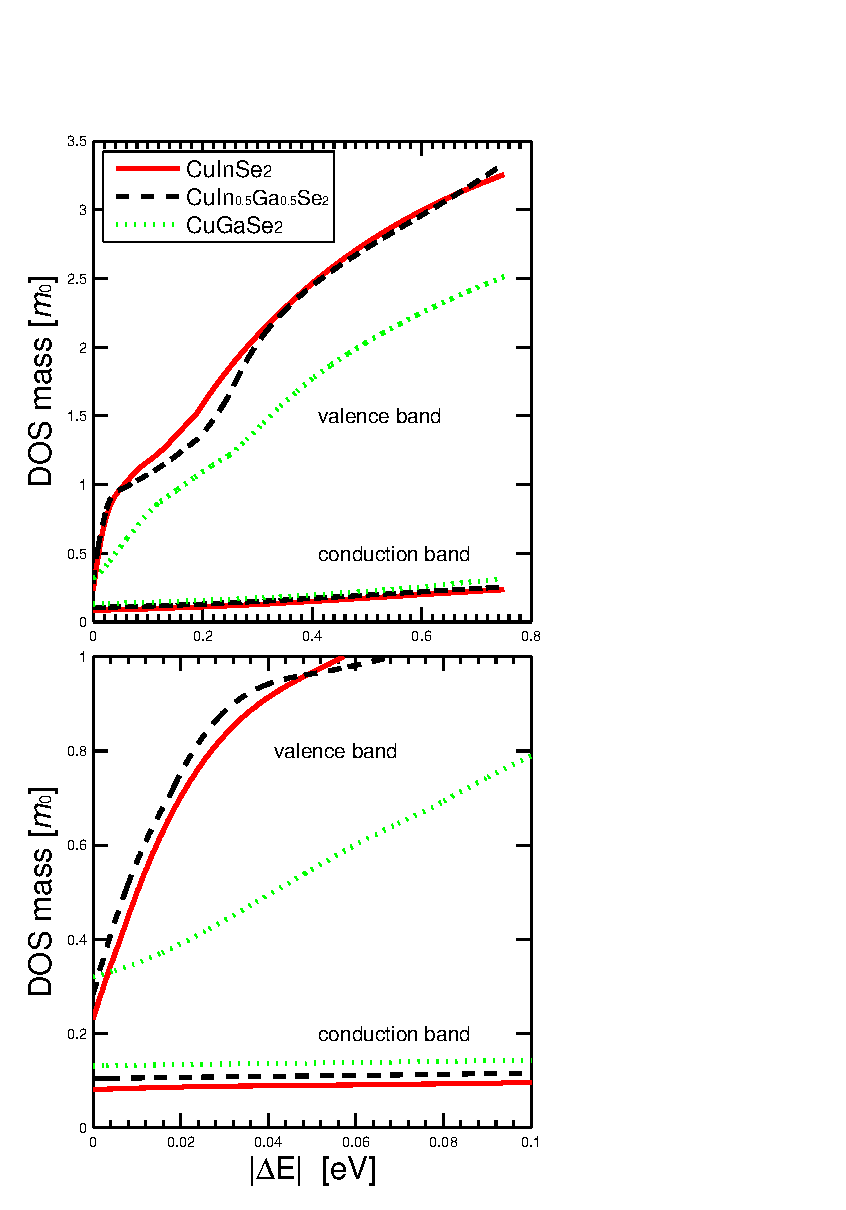
\includegraphics[width=0.46\textwidth,clip]{paper2figure6}
     \end{center}
    \caption{Left: Total DOS of the VBs and CB.The solid lines show the full band parameterization (fbp), and the dashed lines represent the parablolic band approximation (pba).
Right:The DOS mass $m_{v/c}^{DOS}$ is calculated in the equation \ref{dosmass}. }
   \label{dost}
\end{figure}

The \textbf{Fig. \ref{dost}} (left) demonstartes that the non-parabolicity of the bands strongly affect the DOS dispersions. The difference is remarkable. The fbp always
generates larger DOS, the reason is that the non-parablic energy bands is more flat than parabolic bands. The \textbf{Fig. \ref{dost}} (right) demonstrates that the DOS masses of $\cigs$ is strong energy dependence with the VB DOS mass, which proves further the importance of considering 
non-parabolicity and anisotropy of the energy bands, especially for the VBs in the case of $\cigs$. For example, the effecive mass of topmost VB for $CuInSe_2$ is around 
0.23 $m_0$ close to the $\Gamma$ point, which goes up to around 1.00 $m_0$ when $E$ is around 0.1 eV. However, the change in the CB DOS mass is subtle, but also goes up to 2-3 times 
with respect to the value around $\Gamma$ point.

The concentration of free holes $n_v(T)$ and free electrons $n_c(T)$ is calculated by:

\begin{equation}
\begin{split}
& n_v(T) = \int \limits_{-\infty}^{E_{v1}(\textbf{0})} g_v(E)(1-f(E))dE,\\
& n_c(T) = \int \limits_{E_{c1}(0)}^{\infty} g_c(E)f(E)dE, 
\end{split}
\end{equation}

where $f(E) = 1/[1+exp{(E-E_F)/k_BT}]$ is the Fermi disctribution function. The intrinsic carrier concentration can be expressed as:

\begin{equation}\label{cc}
 n_i(T) = \sqrt{n_c(T) \cdot n_v(T)} ,
\end{equation}
 
The extrinsic carrier concentration for p-type materials can be derived as:

\begin{equation}\label{ecc}
n_v(T) = \frac{n_i^2(T)}{n_v(T)} + \sum \limits_{\alpha} \frac{N_{A_{\alpha}}} {1+g_{A_{\alpha}} e^{ (\bigtriangleup_{A_{\alpha}}-E_F)/k_BT }}. 
\end{equation}

where $N_{A_{\alpha}}$ is the acceptor concentration of the $\alpha$th defect, $\bigtriangleup_{A_{\alpha}}$ means the energy level of the acceptor state, and the $g_{A_{\alpha}}$
 is the spin degeneracy factor. The measured ionization energies for $V_{Cu}$ are used from Ref. ??.

The free carrier concentration in intrinsic for $\cigs$ (x = 0, 0.5, and 1) is obtained considering the temperature dependency of the band gaps (Eq. \ref{bgtd}).
The results from the pba for silicon (Si) and GaAs are compared with our simulation as well.

\begin{equation}\label{bgtd}
 E_g(T) = E_g(0) - \frac{a \cdot T^2}{b+T}.
\end{equation}

where parameters $a$ and $b$ are used from experimental values.

 \begin{figure}[H]
    \begin{center}
            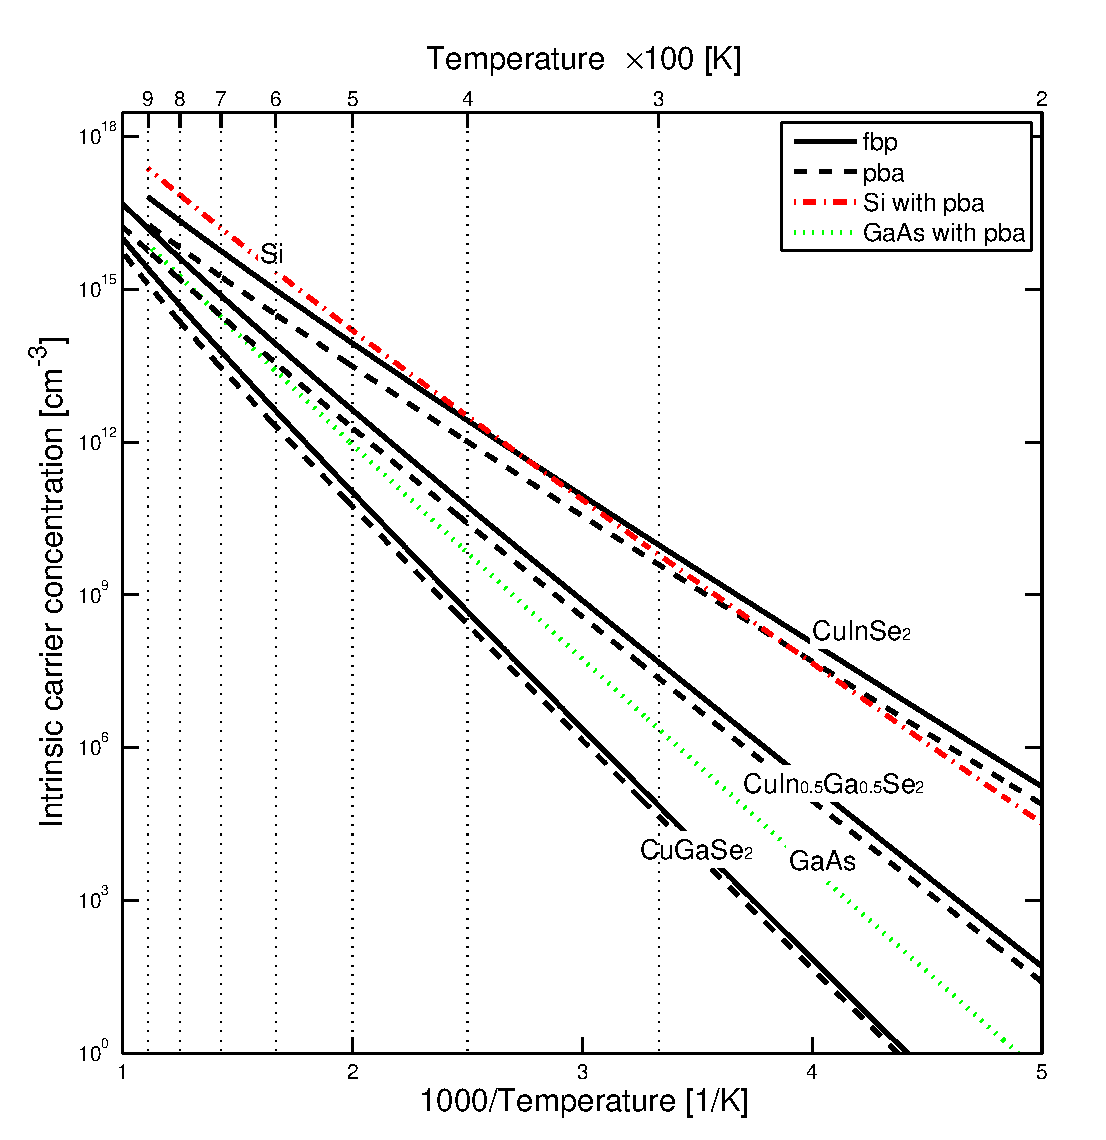
\includegraphics[width=0.5\textwidth,clip]{figure7b_1}
     \end{center}
    \caption{Intrinsic carrier concentration as function of temperature.}
   \label{icc}
\end{figure}

From \textbf{Fig. \ref{icc}}, the free carrier concentration is increased dramatically with the increasing of temperature for the $\cigs$. For example, in the case of $CuInSe_2$, the carrier concentration is
increased up to around $10^{5}$ times higher from temperture 300 K to 600 K. One also notice that the intrinsic carrier concentribution for the Si and $CuInSe_2$ are very comparable. The free carrier concentration is increased 
goes up to 2 - 3 times by taking into account the non-parabolicity of the energy bands. 

The p-type carrier concentration (\textbf{Fig. \ref{ptypecc}}) for $\cigs$ is presented using Eq. \ref{ecc}. 

 \begin{figure}[H]
    \begin{center}
            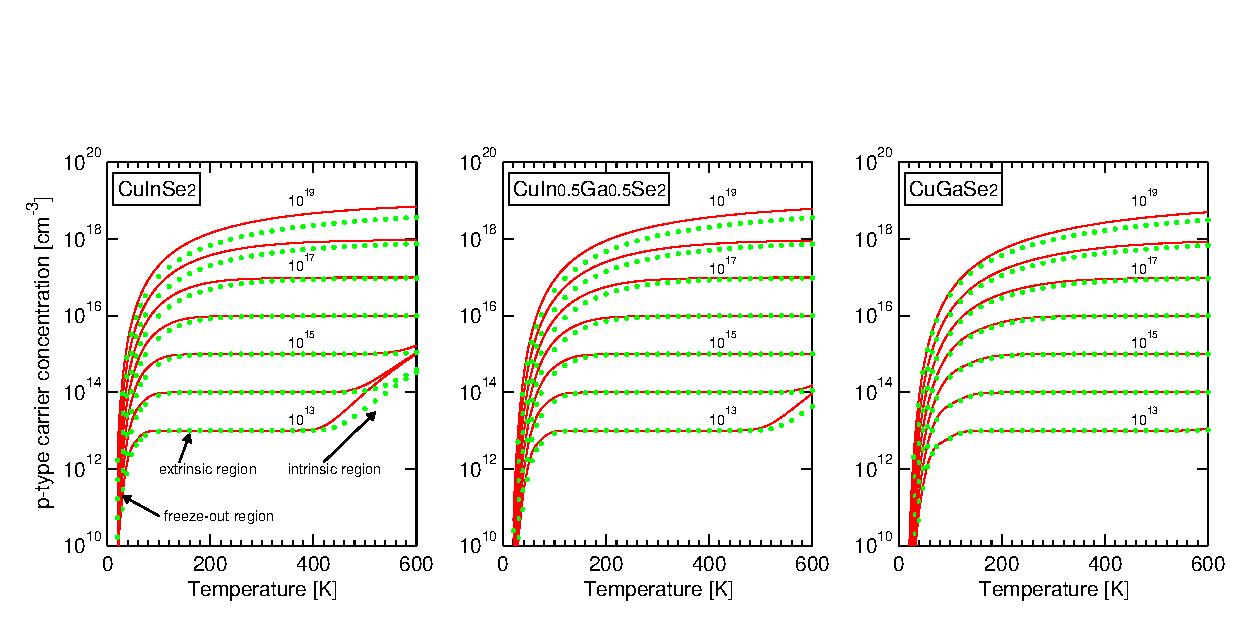
\includegraphics[width=1\textwidth,clip]{paper2figure9}
     \end{center}
    \caption{Free carrier concentration as function of the temperature in p-type for $\mathrm{CuInSe_2}$, $\mathrm{CuIn_{0.5}Ga_{0.5}Se_2}$, and $\mathrm{CuGaSe_2}$.
    The effective doping concentration $N_A = 10^{13}, 10^{14}, 10^{15}$,..., and  $10^{19}$ acceptors/$cm^3$ are considered.}
   \label{ptypecc}
\end{figure}

From \textbf{Fig. \ref{ptypecc}}, the carrier concentration is recognized by three different regions: the freeze-out region, the extrinsic region and the intrinsic region. The 
transition from the freeze-out region to the extrinsic region happens below the room temperature except that the uncompensated acceptor concentration is above around 
$10^{18} cm^{-3}$. The transition from the extrinsic ergion to the intrinsic region for In rich compounds occurs at the lower temperature since they have smaller band gaps.
The result based on the pba underestimates the carrier concentration around by the factor of 2 in the both freeze-out and intrinsic regions. Therefore, the 
non-parabolic energy bands is required in order to describe the carrier concentration more accurately.

\subsubsection{Dielectric function spectra}
In this work, the dielectric function ($\varepsilon$) spectra of $CuIn_{0.5}Ga_{0.5}Se_2$ is calculated by the full-potential linearizaed augmented plane wave (FP-LAPW) method using the generalized gradient approximation (GGA)
plus an onsite Coulomb interaction $U$ of the Cu $d$ states. Afterwards, the different contributions to $\varepsilon_2$ (Im$(\varepsilon)$) in terms of the transitions between the valence bands and the conduction bands are identified. At last, 
the $\textbf{k}$-dependence of the interband critical points (CPs) along the main symmetry directions is analyzed. The result is compared with experimental work ($CuIn_{0.7}Ga_{0.3}Se_2$) at temperature of 40 K and 300 K,
and they are in a good agreement.

 \begin{figure}[H]
    \begin{center}
            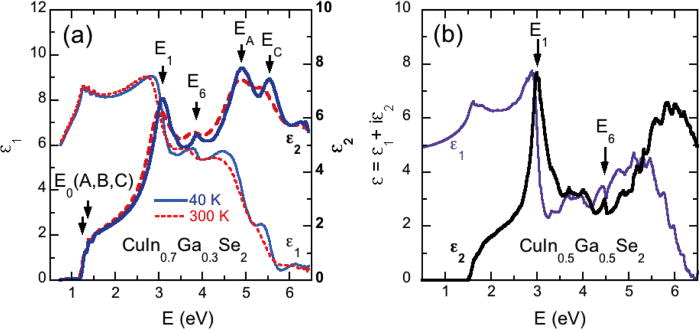
\includegraphics[width=1\textwidth]{111111.png}
     \end{center}
    \caption{Left panel: The real ($\varepsilon_1$) and imaginary ($\varepsilon_2$) part of dielectric function spectra for $CuIn_{0.7}Ga_{0.3}Se_2$ 
at 40 K (solid blue line) and 300 K (dashed red lines). Four prominent CP features are shown. Right panel: the dielectric function spectra for  $CuIn_{0.5}Ga_{0.5}Se_2$
calculated by FP-LAPW method at 0 K. The major CP features are identified. }
   \label{df1}
\end{figure}

From \textbf{Fig. \ref{df1}}, one will notice that the general shape between experimental and calculated result is similar. The calculation indicates that there is no big 
difference in the optical properties for those two materials, except the shift of CP energies.
 
The analysis based on experimental work indicates that there are twelve CPs from 2.5 eV to 6.4 eV. The electronic origin for each CP is analyzed based on the calculated 
result. First, the contribution to dielectric function between the valence bands and conduction bands is presented.

 \begin{figure}[H]
    \begin{center}
            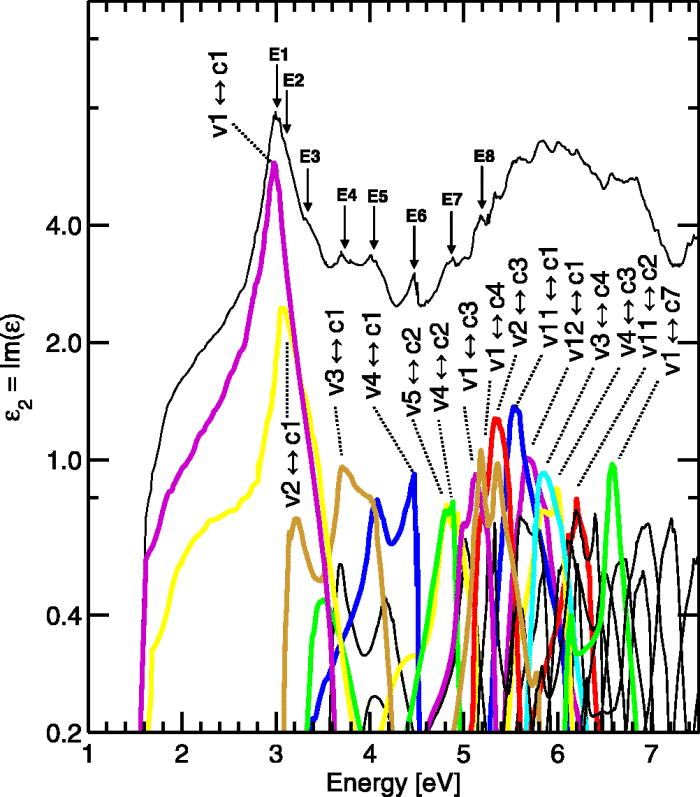
\includegraphics[width=0.5\textwidth]{222222}
     \end{center}
    \caption{Band-to-band analysis of the contribution to the total $\varepsilon_2$ spectrum. The vertical axis is in the log scale.}
   \label{df2}
\end{figure}

where $v_1$ and $c_1$ means the topest valence band and lowest conduction band, respectively. From the \textbf{Fig. \ref{df2}} and \textbf{Fig. \ref{df3}}, one will notice that the $E_1$ CP comes from 
the $v_1 \longrightarrow c_1$
transition near the P(1/2, 1/2, 1/2) point of the brillouin zone (BZ). The $E_2$ and $E_3$ CPs are corresponding to transition of $v_2 \longrightarrow c_1$ in the P point
as well in the BZ.
 The $E_2$ and $E_3$ CPs are small peak in the \textbf{Fig. \ref{df2}}. However, the calculation of $CuInSe_2$ indicates that they happens 0.1-0.2 eV higher than 
the $E_1$ CP, which is distinct spectral features (\textbf{Fig. \ref{ccccc}}). The $E_4$ CP comes from the transition of $v_3 \longrightarrow c_1$ at the $M (1,0,0) = M^*(0,0,1)$ point.
The $E_5$ CP is contributed by the transitions $v_4 \longrightarrow c_1$ at the $N (1/2,0,1/2)$ point and $v_3 \longrightarrow c_1$ at the $M/M^*$ point. The $E_6$ CP feature
corresponding to the  $v_4 \longrightarrow c_1$ at the $N$ point. The $E_7$ is from the transitions $v_4 \longrightarrow c_2$ at the $\Gamma (0,0,0)$ and N point, the 
  $v_5 \longrightarrow c_2$ at the $\Gamma$ point is also contributed.
 \begin{figure}[H]
    \begin{center}
            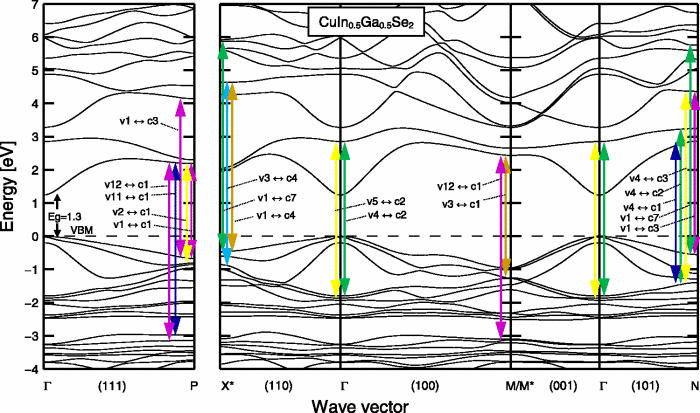
\includegraphics[width=0.8\textwidth]{333333}
     \end{center}
    \caption{Band-to-band analysis of the contribution to the total $\varepsilon_2$ spectrum. The vertical axis is in the log scale.}
   \label{df3}
\end{figure}

\begin{figure}[H]
\begin{center}
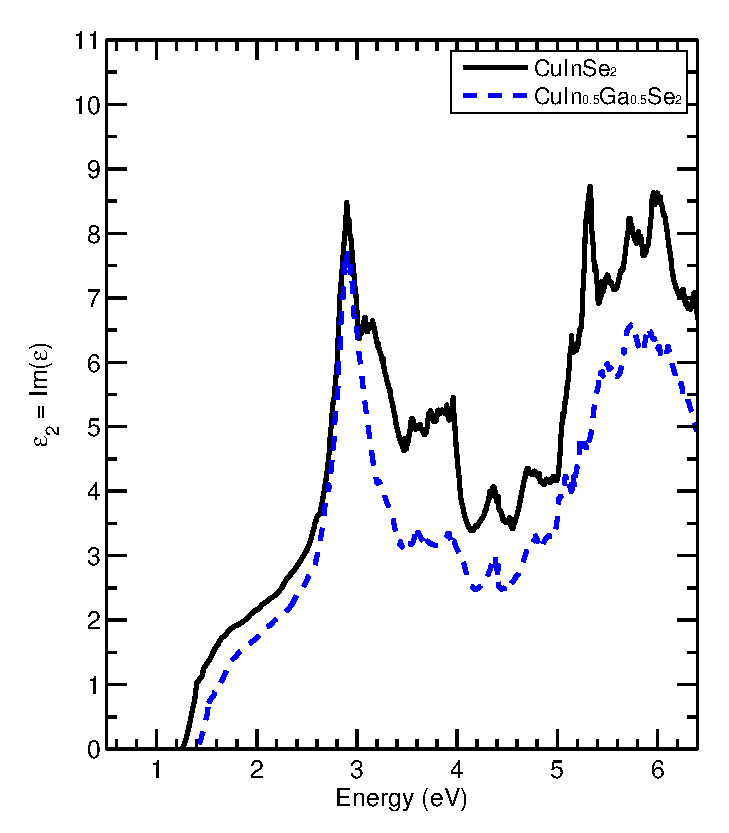
\includegraphics[scale=0.7]{thesis2.eps}
\end{center}
\caption{The $\varepsilon_2$ spectra for ${\mathrm{ CuInSe_2}}$ and $\mathrm {CuIn_{0.5}Ga_{0.5}Se_2}$. }
\label{ccccc}
\end{figure}




\begin{comment}
\section{Methodology and implementation}

\subsection{scalar relativistic approximation}

\subsubsection{Implementation}
In this section, the Hamitonian matrix using scalar relativistic approximation (SRA) term in the Pauli Hamitonian is derived in the muffin tin (MT) 
region and interstitial region (IR). From the section \ref{srasoc}, the SRA Hamitonian term is defined:

\begin{equation}
  H_{sra} = - \frac{\bigtriangledown^4}{8c^2} + \frac{\bigtriangledown^2 V(r)}{8c^2}.
\end{equation}

The Hamitonian matrix can be implemented by:

\begin{equation}
\label{sra1}
 H_{jj'} = \left  < \phi_{j} | H_{sra} | \phi_{{j'}} \right >,
\end{equation}
 
where $\phi_j$ is the basis function. The basis function will be divided into two types in the Exciting code (FP-LAPW method), one is in the muffin tin (MT) region, the other is in the interstitial region. Especially,
the basis function has two forms in the MT region, one is augemented plane wave, another is local orbitals. 

In the MT region, the basis function is:
\begin{equation}
\begin{split}
& \phi_{{\textbf{G}}}^{APW} = \sumg<\alpha>\sum\limits_{{\ell}m} A _{{\ell}m}^{\alpha} {(\textbf{k+G})} u_{{\ell}}(r_{\alpha}, E_{\ell}) Y_{{\ell}m}(\hat{\textbf{r}}_{\alpha}), \\
& \phi_{{{p}}}^{lo} = v_p^{\alpha}(r) Y_{{\ell}_p m_p}(\hat{\textbf{r}}_{\alpha} ) = \sum\limits_{j=1}^{M_p^{\alpha}} B _j^{\alpha} w_j(r_\alpha) Y_{{\ell}_p m_p}(\hat{\textbf{r}}_{\alpha} ),
\end{split}
\end{equation}

where $\phi_{{\textbf{G}}}^{APW}$ and $\phi_{{{p}}}^{lo}$ are the basis function in the MT region. The $A _{{\ell}m}^{\alpha} {(\textbf{k+G})}$ and $B _j^{\alpha}$ are
the match coefficient. The $u_{{\ell}}^{\alpha}(r_{\alpha}, E_{\ell})$ and $w_j(r_\alpha)$ are the radial function, the $Y_{{\ell}m}(\hat{\textbf{r}}_{\alpha})$ and $Y_{{\ell}_p m_p}(\hat{\textbf{r}}_{\alpha})$
are spherical harmonics.

In the interstitial region, the basis function is:
\begin{equation}
 \phi_{{\textbf{G}}}^{IR} =  \frac {1}{\sqrt{\Omega}} e^{i({ \textbf {k+G}}) {\textbf r}}. 
\end{equation}

Therefore the standard Hamitonian matrix (without considering local orbital) in the MT region  is:
\begin{equation}
\label{sra111}
\begin{split}
& H_{jj'}^{MT\_{AA}} =  \left  < \phi_{\textbf{G}}^{APW} | H_{sra} | \phi_{\textbf{G'}}^{APW} \right > 
\end{split}
\end{equation}

In Eq. \ref{sra111}, the main part is to calculate:

\begin{equation}
\label{sra222}
\begin{split}
& \left  < u_{{\ell}}(r_{\alpha}, E_{\ell}) Y_{{\ell}m}(\hat{\textbf{r}}_{\alpha}) | - \frac{\bigtriangledown^4}{8c^2} + \frac{\bigtriangledown^2 V(r)}{8c^2} | u_{{\ell'}}(r_{\alpha}, E_{\ell'}) Y_{{\ell'}m'}(\hat{\textbf{r}}_{\alpha}) \right > \\
& = \left  < u_{{\ell}}(r_{\alpha}, E_{\ell}) Y_{{\ell}m}(\hat{\textbf{r}}_{\alpha}) | - \frac{\bigtriangledown^4}{8c^2} | u_{{\ell'}}(r_{\alpha}, E_{\ell'}) Y_{{\ell'}m'}(\hat{\textbf{r}}_{\alpha}) \right > \\ 
&    + \left  < u_{{\ell}}(r_{\alpha}, E_{\ell}) Y_{{\ell}m}(\hat{\textbf{r}}_{\alpha}) |  \frac{\bigtriangledown^2 V(r)}{8c^2} | u_{{\ell'}}(r_{\alpha}, E_{\ell'}) Y_{{\ell'}m'}(\hat{\textbf{r}}_{\alpha}) \right > \\
& =- \frac{1}{8c^2} \left  < \bigtriangledown^2 \big (u_{{\ell}}(r_{\alpha}, E_{\ell}) Y_{{\ell}m}(\hat{\textbf{r}}_{\alpha}) \big ) | \bigtriangledown^2 \big ( u_{{\ell'}}(r_{\alpha}, E_{\ell'}) Y_{{\ell'}m'}(\hat{\textbf{r}}_{\alpha}) \big )\right > \\
&    + \frac{1}{8c^2} C_{\ell m,\ell'm'}^{\ell_\wedge m_\wedge}\int \limits_{0}^{R_{\alpha}} u_{{\ell}}(r_{\alpha}, E_{\ell}) \overline{V}_{l_\wedge m_\wedge} u_{{\ell'}}(r_{\alpha}, E_{\ell'}) d r \\
& = -\frac{1}{8c^2} \delta_{\ell \ell'}\delta_{m m'} \int \limits_{0}^{R_{\alpha}} \bigtriangledown^2_r u_{{\ell}}(r_{\alpha}, E_{\ell})   \bigtriangledown^2_r u_{{\ell'}}(r_{\alpha}, E_{\ell'}) r_{\alpha}^2 dr \\
& +  \frac{1}{4c^2} \delta_{\ell \ell'}\delta_{m m'} \ell'(\ell'+1) \int \limits_0^{R_{\alpha}} \bigtriangledown_r u_{{\ell}}(r_{\alpha}, E_{\ell}) \bigtriangledown_r u_{{\ell'}}(r_{\alpha}, E_{\ell'}) d r \\
& -  \frac{1}{8c^2} \delta_{\ell \ell'}\delta_{m m'} \ell(\ell+1) \ell(\ell+1) \int \limits_0^{R_{\alpha}}  u_{{\ell}}(r_{\alpha}, E_{\ell})  u_{{\ell'}}(r_{\alpha}, E_{\ell'}) \frac{1}{r_{\alpha}^2} d r \\
& +  \frac{1}{8c^2} C_{\ell m,\ell' m'}^{\ell_\wedge m_\wedge}\int \limits_{0}^{R_{\alpha}} u_{{\ell}}(r_{\alpha}, E_{\ell}) \overline{V}_{l_\wedge m_\wedge} u_{{\ell'}}(r_{\alpha}, E_{\ell'}) r_{\alpha}^2  d r 
\end{split}
\end{equation}

where

\begin{equation}
\begin{split}
& \bigtriangledown^2 \{ V(r) \} \\
& = \bigtriangledown^2 \{ \sum \limits_{\ell_\wedge m_\wedge} V_{\ell_\wedge m_\wedge} Y_{{\ell_\wedge } m_\wedge}(\hat{\textbf{r}}_{\alpha})\} \\
& = \sum \limits_{\ell_\wedge m_\wedge} \overline{V}_{\ell_\wedge m_\wedge} Y_{{\ell_\wedge } m_\wedge}(\hat{\textbf{r}}_{\alpha}),
\end{split}
\end{equation}

and $C_{\ell m,\ell' m'}^{\ell_\wedge m_\wedge}$ in equation \ref{sra222} is the Gaunt coefficients.

It is similar to consider the local orbitals:

\begin{equation}
\begin{split}
& H_{jj'}^{MT\_{ALo}} =  \left  < \phi_{\textbf{G}}^{APW} | H_{sra} | \phi_{p}^{lo} \right > 
\end{split}
\end{equation}

The main part to be calculated is:

\begin{equation}
\label{sra333}
\begin{split}
& \frac{1}{8c^2} \left  < \bigtriangledown^2 \big (u_{{\ell}}(r_{\alpha}, E_{\ell}) Y_{{\ell}m}(\hat{\textbf{r}}_{\alpha}) \big ) | \bigtriangledown^2 \big (w_j(r_\alpha)) Y_{{\ell_p}m_p}(\hat{\textbf{r}}_{\alpha}) \big )\right > \\
&    + \frac{1}{8c^2} C_{\ell m,\ell_p m_p}^{\ell_\wedge m_\wedge}\int \limits_{0}^{R_{\alpha}} u_{{\ell}}(r_{\alpha}, E_{\ell}) \overline{V}_{l_\wedge m_\wedge} w_j(r_\alpha) d r \\
& = -\frac{1}{8c^2} \delta_{\ell \ell_p}\delta_{m m_p} \int \limits_{0}^{R_{\alpha}} \bigtriangledown^2_r u_{{\ell}}(r_{\alpha}, E_{\ell})   \bigtriangledown^2_r w_j(r_\alpha) r_{\alpha}^2 dr \\
& +  \frac{1}{4c^2} \delta_{\ell \ell_p}\delta_{m m_p} \ell_p(\ell_p+1) \int \limits_0^{R_{\alpha}} \bigtriangledown_r u_{{\ell}}(r_{\alpha}, E_{\ell}) \bigtriangledown_r w_j(r_\alpha)   d r \\
& -  \frac{1}{8c^2} \delta_{\ell \ell_p}\delta_{m m_p} \ell(\ell+1) \ell_p(\ell_p+1) \int \limits_0^{R_{\alpha}}  u_{{\ell}}(r_{\alpha}, E_{\ell}) w_j(r_\alpha) \frac{1}{r_{\alpha}^2} d r \\
& +  \frac{1}{8c^2} C_{\ell m,\ell_p m_p}^{\ell_\wedge m_\wedge}\int \limits_{0}^{R_{\alpha}} u_{{\ell}}(r_{\alpha}, E_{\ell}) \overline{V}_{l_\wedge m_\wedge} w_j(r_\alpha) r_{\alpha}^2  d r. 
\end{split}
\end{equation}

And

\begin{equation}
\begin{split}
& H_{jj'}^{MT\_{LoA}} =  \left  < \phi_{p}^{lo}   | H_{sra} | \phi_{\textbf{G}}^{APW} \right > 
\end{split}
\end{equation}
The main part to be calculated is:

\begin{equation}
\label{sra222}
\begin{split}
&  \left  < w_j(r_\alpha) Y_{{\ell_p}m_p}(\hat{\textbf{r}}_{\alpha}) | - \frac{\bigtriangledown^4}{8c^2} | u_{{\ell'}}(r_{\alpha}, E_{\ell'}) Y_{{\ell'}m'}(\hat{\textbf{r}}_{\alpha}) \right > \\ 
&    + \left  <  w_j(r_\alpha) Y_{{\ell_p}m_p}(\hat{\textbf{r}}_{\alpha}) |  \frac{\bigtriangledown^2 V(r)}{8c^2} | u_{{\ell'}}(r_{\alpha}, E_{\ell'}) Y_{{\ell'}m'}(\hat{\textbf{r}}_{\alpha}) \right > \\
& = \frac{1}{8c^2} \left  < \bigtriangledown^2 \big ( w_j(r_\alpha) Y_{{\ell_p}m_p}(\hat{\textbf{r}}_{\alpha}) \big ) | \bigtriangledown^2 \big ( u_{{\ell'}}(r_{\alpha}, E_{\ell'}) Y_{{\ell'}m'}(\hat{\textbf{r}}_{\alpha}) \big )\right > \\
&    + \frac{1}{8c^2} C_{\ell_p m_p,\ell'm'}^{\ell_\wedge m_\wedge}\int \limits_{0}^{R_{\alpha}} w_j(r_\alpha) \overline{V}_{l_\wedge m_\wedge} u_{{\ell'}}(r_{\alpha}, E_{\ell'}) d r \\
& = - \frac{1}{8c^2} \delta_{\ell_p \ell'}\delta_{m_p m'} \int \limits_{0}^{R_{\alpha}} \bigtriangledown^2_r w_j(r_\alpha)   \bigtriangledown^2_r u_{{\ell'}}(r_{\alpha}, E_{\ell'}) r_{\alpha}^2 dr \\
& +  \frac{1}{4c^2} \delta_{\ell_p \ell'}\delta_{m_p m'} \ell'(\ell'+1) \int \limits_0^{R_{\alpha}} \bigtriangledown_r w_j(r_\alpha) \bigtriangledown_r u_{{\ell'}}(r_{\alpha}, E_{\ell'}) d r \\
& -  \frac{1}{8c^2} \delta_{\ell_p \ell'}\delta_{m_p m'} \ell_p(\ell_p+1) \ell'(\ell'+1) \int \limits_0^{R_{\alpha}}  w_j(r_\alpha)  u_{{\ell'}}(r_{\alpha}, E_{\ell'}) \frac{1}{r_{\alpha}^2} d r \\
& +  \frac{1}{8c^2} C_{\ell_p m_p,\ell' m'}^{\ell_\wedge m_\wedge}\int \limits_{0}^{R_{\alpha}} w_j(r_\alpha) \overline{V}_{l_\wedge m_\wedge} u_{{\ell'}}(r_{\alpha}, E_{\ell'}) r_{\alpha}^2  d r 
\end{split}
\end{equation}

And 

\begin{equation}
\begin{split}
& H_{jj'}^{MT\_{LoLo}} =  \left  <\phi_{p}^{lo}  | H_{sra} | \phi_{p'}^{lo} \right > 
\end{split}
\end{equation}
The main part to be calculated is:

\begin{equation}
\label{sra444}
\begin{split}
& \frac{1}{8c^2} \left  < \bigtriangledown^2 \big (w_j(r_\alpha) Y_{{\ell_p}m_p}(\hat{\textbf{r}}_{\alpha}) \big ) | \bigtriangledown^2 \big (w_{j'}(r_\alpha)) Y_{{\ell_{p'}}m_{p'}}(\hat{\textbf{r}}_{\alpha}) \big )\right > \\
&    + \frac{1}{8c^2} C_{\ell_p m_p,\ell_{p'} m_{p'}}^{\ell_\wedge m_\wedge}\int \limits_{0}^{R_{\alpha}} w_j(r_\alpha) \overline{V}_{l_\wedge m_\wedge} w_{j'}(r_\alpha) d r \\
& = - \frac{1}{8c^2} \delta_{\ell_p \ell_{p'}}\delta_{m_p m_{p'}} \int \limits_{0}^{R_{\alpha}} \bigtriangledown^2_r w_j(r_\alpha)   \bigtriangledown^2_r w_{j'}(r_\alpha) r_{\alpha}^2 dr \\
& +  \frac{1}{8c^2} \delta_{\ell_p \ell_{p'}}\delta_{m_p m_{p'}} \ell_{p'}(\ell_{p'}+1) \int \limits_0^{R_{\alpha}} \bigtriangledown_r w_j(r_\alpha) \bigtriangledown_r w_{j'}(r_\alpha) d r \\
& -  \frac{1}{8c^2} \delta_{\ell_p \ell_{p'}}\delta_{m_p m_{p'}} \ell_{p}(\ell_{p}+1) \ell_{p'}(\ell_{p'}+1) \int \limits_0^{R_{\alpha}}  w_j(r_\alpha) w_{j'}(r_\alpha) \frac{1}{r_{\alpha}^2} d r \\
& +  \frac{1}{8c^2} C_{\ell_p m_p,\ell_{p'} m_{p'}}^{\ell_\wedge m_\wedge}\int \limits_{0}^{R_{\alpha}} w_j(r_\alpha) \overline{V}_{l_\wedge m_\wedge} w_{j'}(r_\alpha) r_{\alpha}^2 d r 
\end{split}
\end{equation}

In the interstial region:

\begin{equation}
\begin{split}
& H_{jj'}^{IR} =  \left  < \phi_{\textbf{j}}^{IR} | H_{sra} | \phi_{\textbf{j'}}^{IR} \right > \\
&              = \left  < \phi_{{\textbf{G}}}^{IR}  | H_{sra} | \phi_{{\textbf{G'}}}^{IR} \right > \\
&              =  \frac{1}{{8 {c}^2 }} \{ -(k+G)^2(k+G')^2 \widetilde{\theta}_{I}(G-G') -  \sumg<G''> V_{G''}(G'')^2 \widetilde{\theta}_{I}(G-G'-G'') \}
\end{split}
\end{equation}

where potential is defined in the section \ref{epote}. And if $\theta_{I}(r)$ is the characteristic function of the interstitial region ( $r$ included in MT, $\theta_{I}(r)$ = 0, otherwise it is 1), $\widetilde{\theta}_{I}(r)$ comes from the Fourier transform of $\theta_{I}(r)$:
\begin{equation}
\theta_{I}(r) = \sumg<G> \widetilde{\theta}_{I}(G) \expg<G>
\end{equation}

And $\widetilde{\theta}_{I}(G)$ is defined:
 
\begin{equation*}\label{ap1}
\widetilde{\theta}_{I}(G) =
\begin{cases}  \delta_{G,0}-\sumg<\alpha> \frac{4 \pi R_{\alpha}^{3}}{\Omega} \frac{j_1(|G|R_{\alpha})}{|G|R_{\alpha}} e^{-iGr_{\alpha}} & \quad \mbox{if $\textbf{G} \leqslant \textbf{G}_{max} $}
\\
0  & \quad \mbox{if $\textbf{G} > \textbf{G}_{max} $}\\ 
\end{cases}
\end{equation*}

where $R_{\alpha}$ is the radius of the MT, $r_{\alpha}$ is the position refer to the $\alpha$th atom, and $j_1$ is the ${1}$st order Bessel function.

\subsubsection{Results and discusstion}
It is needed to insert more after getting some results.

\subsection{Scalar relativistic approximation in k $\cdot$ p method}
\subsubsection{Implementation}
One can check the section \ref{kpmaa} for the introduction of \textbf{k $\cdot$ p} method. Here the relativistic KS equation for \textbf{k $\cdot$ p} method in atomic units can be expressed as:

\begin{equation}\label{m1}
\left\{ - \frac{\bigtriangledown^2}{2} + V(r) - \frac{\bigtriangledown^4}{8c^2} + \frac{\bigtriangledown^2 V(r)}{8c^2} \right\} \wfbloch<n>< \bold k> = \ebloch<n><\bold k> \wfbloch<n><\bold k>,
\end{equation}

where 

\begin{equation}\label{m2}
\begin{split}
& \wfbloch<n><\bold k> =  {\sum\limits_{j}} C_{n,j}^{\bold k} \chikp<j><\bold k>, \\
& \chikp<j><\textbf k> = \expg<(\bold k-\bold {k_0})>  \wfbloch<j><\bold {k_0}>.
\end{split}
\end{equation}

One can follow almost the same derivation but with more terms in the section \ref{kpmaa}, which ends up:

\begin{equation}\label{m4}
{\sum\limits_{j}} C_{n,j}^{\bold {k}} \left \{ H_{j',j}- \ebloch<n><\bold {k}> \delta_{j',j} \right \} =0,
\end{equation}

where
\begin{equation} \label{m5}
\begin{split}
& H_{j',j} = \left \{  \ebloch<j><\bold {k_0}>  + \frac{1}{2} { (\bold{k}-\bold{k}_0)^2} - \frac{1}{8c^2}(\bold{k}-\bold{k}_0)^4   \right \} \delta_{j',j} + \left \{ {-i(\bold{k}-\bold{k}_0) + \frac{i}{2c^2}(\bold{k}-\bold{k}_0)^3} \right \} {\textbf p_{j',j}} \\
& \qquad  + \left \{ \frac{3}{4c^2}(\bold{k}-\bold{k}_0)^2  \right \} {\textbf p'_{j',j}} + \left \{ \frac{-i}{2c^2}(\bold{k}-\bold{k}_0) \right \} {\textbf p''_{j',j}}, 
\end{split}
\end{equation}

and

\begin{equation} 
\begin{split}
& {\textbf p_{j',j}} = \langle \wfbloch<j'>< \bold k_0>| {\bigtriangledown} | \wfbloch<j>< \bold k_0>  \rangle, \\
& {\textbf p'_{j',j}} = \langle \wfbloch<j'>< \bold k_0>| {\bigtriangledown^2} | \wfbloch<j>< \bold k_0>  \rangle, \\
& {\textbf p''_{j',j}} = \langle \wfbloch<j'>< \bold k_0>| {\bigtriangledown^3} |\wfbloch<j>< \bold k_0>  \rangle.
\end{split}
\end{equation}

From the above Eq. \ref{m4}, the coefficient $ C_{n,j}^{\bold k}$ and $\ebloch<n><\bold {k}>$ are calculated.

\subsubsection{Results and discussion}

It is needed to insert more after getting some results.

\subsection{Spin-orbit coupling}

\subsubsection{Implementation}
In this section, spin-orbit coupling (SOC) implementation is derived in the muffin tin (MT) region and interstial region (IR). In the MT region, this implementation is compared with 
the method exsiting in the orignal Exciting code.

First, the way to implemente the SOC in the Exciting code is presented, which is included in second-variational scheme, that means it takes use of the basis function which is expanded from the first variational wavefunction.
\begin{equation}
\begin{split}
 & \widehat{H}_{1}   \phi^{i}_{1}  = E^{i}_1  \phi^{i}_{1} \\
 & (\widehat{H}_1+\widehat{H}_{soc})  \Psi  = E \Psi
\end{split}
\end{equation}
\noindent  where $ \widehat{H}_{1}$ and $ \phi^{i}_{1}$ are first variational \hm and wavefunction, respectively, and $\Psi = \sumi<i> c_{i} \phi^{i}_1$.
If  multiply $\phi^{j}_{1}$ on the left side of the second item of the above equation.
\begin{equation}
\begin{split}
 & <  \phi^{j}_1 |(\widehat{H}_1+\widehat{H}_{soc}) | \sumi<i> c_{i} \phi^{i}_1 > = E< \phi^{j}_1 | \sumi<i> c_{i} \phi^{i}_1>
\end{split}
\end{equation}

\noindent After some operations, the above equation becomes:
\begin{equation}
\begin{split}
 &\sumi<i> c_{i} \{ E^{i}_{1} \delta_{i,j} +<\phi^{j}_1 |\widehat{H}_{soc} | \phi^{i}_1  > \} = \sumi<i> c_{i} E \delta_{i,j}
\end{split}
\end{equation}
 
\noindent So finally, the above equation becomes the eigenvalue probelm $H_2 C = E C$.
\begin{equation}\label{ep444}
H_2=\left[
\begin{matrix}
    E_1+H_{11} & H_{12} & \cdots & H_{1N} \\
    H_{21} & E_2 + H_{22} & \cdots & H_{2N} \\
    \vdots               & \vdots               &        & \vdots               \\
     H_{N1} & H_{N2} & \cdots & E_{N}+H_{NN} \\
\end{matrix} \right],
C = \left[ \begin{array}{c} c_1 \\ c_2 \\ \vdots \\ c_N\end{array} \right]
\end{equation}

where $H_{j,j'} = <\phi^{j}_1 |\widehat{H}_{soc} | \phi^{j'}_1  > $. 

In the current Exciting code, the SOC in the MT region is implemented by the term expressed: 
\begin{equation}
 H_{soc}^{1} = \frac{1}{4M^2c^2} \frac{1}{r} \frac{dV(r)}{dr} \boldsymbol{\sigma}{L},
\end{equation}

where $M=1-{V(r)}/{(2c^2)}$ and V(r)=$V_{\ell=0,m=0}(r)$. 

In this section, another expression is utilized, 
\begin{equation}
\label{socterm}
 H_{soc}^2 = \frac{1}{4 c^2} \boldsymbol{\sigma}[\nabla{V(r)} \times \textbf{P}],
\end{equation}

where $V(r)$ is general potential, which means that V(r) = $V_{\ell,m}(r)$, here $\ell$ and $m$ could be greater than zero.


From Eq. \ref{ep444}, one can notice that the main part is to calculate $H_{j,j'} = <\phi^{j}_1 |\widehat{H}_{soc} | \phi^{j'}_1  > $.

Before going furture derivation, first, some equalities need to be presented:

\begin{equation}
\begin{split}
& \sigma \cdot \textbf{h} = \left (  \begin{array}{ccc}
h_z & h_x-ih_y\\
h_x+ih_y & -h_z\end{array} \right ), \\
& \textbf{A} \times \textbf{B} = \left ( A_x B_x, A_y B_y, A_z B_z  \right ).
\end{split}
\end{equation}

Also, there is one way to calculate the gradient of muffin-tin function, for example, 
\begin{equation}
 F(r) = \sum \limits_{\ell m} f_{\ell m}(\textbf{r}) Y_{\ell m} (\textbf{r}_{\alpha}),
\end{equation}

where $F(r)$ is muffin tin function, then, the gradient of this function could be expressed by: 
\begin{equation}
 \bigtriangledown F(r) = \sum \limits_{\ell m} \overline{f}_{\ell m}(\textbf{r}) Y_{\ell m} (\textbf{r}_{\alpha}).
\end{equation}

One will notice that the wavefunction and potential in the MT region here also can be constructed to be similar form like $F(r)$.

Now it is the time to calculate the SOC Hamiltonian matrix (in atomic units):

\begin{equation}
\label{soc12345}
\begin{split}
& H_{j,j'} = <\phi^{j}_1 |\widehat{H}_{soc} | \phi^{j'}_1  > \\
&          = < \sum \limits_{\ell m} G_{\ell m}^j Y_{\ell m} (\textbf{r}_\alpha)| - \frac{i}{4 c^2} \boldsymbol{\sigma} \cdot [\nabla{V(r)} \times \nabla] | \sum \limits_{\ell' m'} G_{\ell m}^{j'} Y_{\ell' m'} (\textbf{r}_\alpha)> \\
&          =  - \frac{i}{4 c^2} < \sum \limits_{\ell m} G_{\ell m}^j Y_{\ell m} (\textbf{r}_\alpha)| \boldsymbol{\sigma} \cdot  \nabla \left ( {\sum \limits_{\ell_\wedge m_\wedge}V_{\ell_\wedge m_\wedge} Y_{\ell_\wedge m_\wedge} (r_\alpha)} \right ) \times \nabla \left ( \sum \limits_{\ell' m'} G_{\ell' m'}^{j'} Y_{\ell' m'} (\textbf{r}_\alpha) \right)> \\
&          = - \frac{i}{4 c^2} \sum \limits_{\ell m, \ell' m'}^{\ell_\wedge m_\wedge} C_{\ell m,\ell' m'}^{\ell_\wedge m_\wedge} < G_{\ell m}^j | \sigma \cdot \overline{V}_{\ell_\wedge m_\wedge} \times   \overline{G}_{\ell' m'}^{j'}> \\
&          =- \frac{i}{4 c^2} \sum \limits_{\ell m, \ell' m'}^{\ell_\wedge m_\wedge} C_{\ell m,\ell' m'}^{\ell_\wedge m_\wedge} < G_{\ell m}^j | \sigma \cdot \overline{M}_{\ell_\wedge m_\wedge}^{\ell' m'} > \\
&          = - \frac{i}{4 c^2} \sum \limits_{\ell m, \ell' m'}^{\ell_\wedge m_\wedge} C_{\ell m,\ell' m'}^{\ell_\wedge m_\wedge} < G_{\ell m}^j | \left (  \begin{array}{ccc}
\overline{M}_z & \overline{M}_x-i\overline{M}_y\\
\overline{M}_x+i\overline{M}_y & -\overline{M}_z\end{array} \right ) >,
\end{split}
\end{equation}

where $\overline{M}_{\ell_\wedge m_\wedge}^{\ell' m'} = \overline{V}_{\ell_\wedge m_\wedge} \times   \overline{G}_{\ell' m'}^{j'}$, and the wavefunction and potential and gradient of them in the MT region are:
\begin{equation}
\begin{split}
& \phi^{j'}_1 = \sum \limits_{\ell' m'} G_{\ell' m'}^{j'} Y_{\ell' m'} (\textbf{r}_\alpha), \\
& \nabla \phi^{j'}_1 = \sum \limits_{\ell' m'} \overline{G}_{\ell' m'}^{j'} Y_{\ell' m'} (\textbf{r}_\alpha), \\
& V(r) = {\sum \limits_{\ell_\wedge m_\wedge}V_{\ell_\wedge m_\wedge} Y_{\ell_\wedge m_\wedge} (r_\alpha)}, \\
& \nabla V(r) = {\sum \limits_{\ell_\wedge m_\wedge} \overline{V}_{\ell_\wedge m_\wedge} Y_{\ell_\wedge m_\wedge} (r_\alpha)}
\end{split}
\end{equation}

Since the there are spin up and spin down, therefore, the Hamiltonian matrix is divided by the 2 $\times$ 2 matrix,
 each block of the matrix means the combination matrix from spin up and down :

\begin{equation}\label{block}
 \left( \begin{array}{cc}
\uparrow \uparrow & \uparrow \downarrow\\
\downarrow \uparrow & \downarrow \downarrow \end{array} \right)
\rightarrow \left (  \begin{array}{ccc}
\overline{M}_z & \overline{M}_x-i\overline{M}_y\\
\overline{M}_x+i\overline{M}_y & -\overline{M}_z\end{array} \right ) 
\end{equation}

where $\downarrow$ and $\uparrow$ represent spin down and up, respectively.

Therefore, the Eq. \ref{soc12345} could be further derived:

For the case of spin up to spin up ($\uparrow \uparrow$):
\begin{equation}
H_{j,j'} =  - \frac{i}{4 c^2} \sum \limits_{\ell m, \ell' m'}^{\ell_\wedge m_\wedge} C_{\ell m,\ell' m'}^{\ell_\wedge m_\wedge} < G_{\ell m}^j | \overline{M}_z>
\end{equation}

For the case of spin down to spin down ($\downarrow \downarrow$):
\begin{equation}
H_{j,j'} =  - \frac{i}{4 c^2} \sum \limits_{\ell m, \ell' m'}^{\ell_\wedge m_\wedge} C_{\ell m,\ell' m'}^{\ell_\wedge m_\wedge} < G_{\ell m}^j | -\overline{M}_z>
\end{equation}

For the case of spin up to spin down ($\uparrow \downarrow$):
\begin{equation}
H_{j,j'} =  - \frac{i}{4 c^2} \sum \limits_{\ell m, \ell' m'}^{\ell_\wedge m_\wedge} C_{\ell m,\ell' m'}^{\ell_\wedge m_\wedge} < G_{\ell m}^j | \overline{M}_x-i\overline{M}_y>
\end{equation}

From now on, the SOC implementation in the IR is derived. The Hamiltonian matrix utilizing the SOC term in Eq. \ref{socterm} is not Hermitian matrix. Therefore, here a new 
method is imported, named ZORA term. It has the following form:

It is not finished yet this part! and the non-hermitian using the SOC term in Eq. \ref{socterm} needs to be tested carefully!!! 





\subsubsection{Results and discussion}
It is needed to insert more after getting some results.

\end{comment}


\chapter{Concluding remarks and future work}

\chapter*{Acknowledgements} \addcontentsline{toc}{chapter}{Acknowledgements}


\end{document}
